% PREAMBULE

%package obligatoire : type de document
\documentclass[a4paper,12pt,twoside]{book}

% encodage
\usepackage{fontspec}

% le package hyperref avec des options, si en local

%\usepackage[pdfusetitle, pdfsubject ={Mémoire TNAH}, pdfkeywords={les mots-clés}]{hyperref}

%avec overleaf, utiliser :
\usepackage[xetex]{hyperref}
\hypersetup{
	pdfauthor = {Esteban Sánchez Oeconomo},
    pdftitle =  {Du catalogue papier au tableur numérique},
	pdfsubject = {sujet},
	pdfkeywords = {catalogues} {histoire de l'art} {python} {OCR} {extraction} {ALTO} {TEI} {CSV}
}

%il faut mettre au moins une langue
\usepackage[main=french, english]{babel}
\usepackage{csquotes} % pour que les citations biblatex soient correctes et éviter un message d'erreur

% configurer le document selon les normes de l'école
\usepackage[margin=2.5cm]{geometry} %marges
\usepackage{setspace} % espacement qui permet ensuite de définir un interligne
\onehalfspacing % interligne de 1.5
\setlength\parindent{1cm} % indentation des paragraphes à 1 cm

\usepackage{lettrine} % lettrines (pas obligatoire)


% bibliographie
\usepackage[backend=biber, sorting=nyt, style=enc,maxbibnames=10]{biblatex}
\addbibresource{TNAHmemoire.bib}
\nocite{*}

%si index, package pour index + makeindex

% + toutes la liste des packages nécessaires à votre document (si images, tableaux, schémas, etc.)
\usepackage{graphicx}
\graphicspath{ {./images_notebook/} {./images_memoire/} {./images_memoire/decoupes/}  } 
\usepackage{wrapfig}
\usepackage[rightcaption]{sidecap}
\usepackage{subcaption}
\usepackage[acronym, nonumberlist]{glossaries}
\usepackage{verbatim} % permet de faire des commentaires sur plusieurs lignes
\usepackage{minted}   % pour montrer du code comme tel
\usepackage{enumitem} % ici et en bas, c'est un paquet pour les listes, qui permet d'avoir un espace blanc après la liste
\setlist{noitemsep}


\makenoidxglossaries
\newacronym{ocr}{OCR}{Optical Character Recognition}
\newacronym{htr}{HTR}{Handwritten Character Recognition}
\newacronym{tei}{TEI}{Text Encoding Initiative}
\newacronym{xml}{XML}{eXtensible Markup Language}
\newacronym{xslt}{XSLT}{eXtensible Stylesheet Language Transformations}
\newacronym{grobid}{GROBID}{GeneRation Of BIbliographic Data}
\newacronym{alto}{ALTO}{Analysed Layout and Text Object}
%\newacronym{page}{PAGE}{Page Analysis and Ground truth Elements}
\newacronym{odd}{ODD}{One Document Does it all}
\newacronym{pdf}{PDF}{Portable Document Format}
\newacronym{iiif}{IIIF}{International Image Interoperability Framework}
\newacronym{csv}{CSV}{Comma Separated Values}
\glsaddall[]

\pagestyle{plain}


% on pourra aussi utiliser la commande mise dans l'exemple de correction du TP1 pour enlever les titres courant qui traînent sur les pages

\author{Esteban Sánchez - M2 TNAH}
\title{Du catalogue papier au tableur numérique. Un pipeline semi-automatique pour former des étudiants en sciences humaines aux humanités numériques}
\begin{document}
	

	\begin{titlepage}
	\begin{center}
		
		\bigskip
		
		\begin{large}				
			ÉCOLE NATIONALE DES CHARTES\\
			UNIVERSITÉ PARIS, SCIENCES \& LETTRES
		\end{large}
		\begin{center}\rule{2cm}{0.02cm}\end{center}
		
		\bigskip
		\bigskip
		\bigskip
		\begin{Large}
			\textbf{Esteban Sánchez Oeconomo}\\
		\end{Large}
		%selon le cas
		\begin{normalsize} 
			\textit{licencié ès lettres}
			
			\textit{diplômé de master}
		\end{normalsize}
		
		\bigskip
		\bigskip
		\bigskip
		
		\begin{Huge}
			\textbf{Du catalogue papier au tableur numérique.}\\
		\end{Huge}
		\bigskip
		\bigskip
		\begin{LARGE}
			\textbf{Un pipeline semi-automatique pour former des étudiants en sciences humaines aux humanités numériques}\\
		\end{LARGE}
		
		\bigskip
		\bigskip
		\bigskip
		\begin{large}
		\end{large}
		\vfill
		
		\begin{large}
			Mémoire 
			pour le diplôme de master \\
			\og{} Technologies numériques appliquées à l'histoire \fg{} \\
			\bigskip
			2022
		\end{large}
		
	\end{center}
\end{titlepage}

\thispagestyle{empty}	
\cleardoublepage

\frontmatter
\chapter{Résumé}

\medskip

Le présent mémoire établi un premier bilan pour un stage effectué pendant l'été 2022 à l'Université de Genève, sous la direction de Béatrice Joyeux-Prunel et de Simon Gabay. Financée par l'École normale supérieure et par le centre IMAGO, cette mission s'est déroulée au sein du projet Artl@s, qui vise à cartographier les circulations artistiques mondiales des XIXe et XXe siècles.\\

Ce travail présente une chaîne de traitement semi-automatique pour extraire des données contenues dans des catalogues d'expositions d'art du XIXe et XXe siècles. Il s'intéresse à ses enjeux scientifiques, pédagogiques et plus largement techniques. Il propose de positionner la mission dans un processus dilaté sur trois stages effectués depuis 2019, en prenant soin de comprendre les continuités et les ruptures qui ont mené à définir une direction résolument tournée vers l'accessibilité de l'outil.

Le pipeline développé vise à produire efficacement des données pour la recherche, mais sa vocation fondamentale est pédagogique : l'outil a été conçu pour introduire des étudiants en sciences humaines aux principaux outils des humanités numériques. Ce mémoire suggère que le livrable développé mène, pour la première fois, à remplir un objectif défini depuis le début des stages : permettre aux collaborateurs du projet de produire des données satisfaisantes à partir d'un programme simple et solide qui leur transmette les notions techniques fondamentales des humanités numériques.\\



\textbf{Mots-clés~:} Artl@s; catalogues; histoire de l’art; OCR; Python ; XML-ALTO ; XML-TEI; CSV

\textbf{Informations bibliographiques~:} Esteban Sánchez Oeconomo, \textit{Du catalogue papier au tableur numérique. Un pipeline semi-automatique pour former des étudiants en sciences humaines aux humanités numériques}, mémoire de master \og{}Technologies numériques appliquées à l'histoire\fg{}, dir. Béatrice Joyeux-Prunel et Simon Gabay, École nationale des chartes, 2022.

\chapter{Remerciements}


"Tu finis ton master, hein ?"\\

\lettrine{J}e dédie mon travail à ma mère, à qui j'ai promis que je terminerais cette formation.\\

Ce travail, et de manière plus large l'ensemble de mon parcours de M2, n'auraient pas été menés à terme sans l'aide spontanée de l'équipe pédagogique et administrative du master TNAH et de mes responsables de stage. Leur compréhension m'a permis de tenir un engagement que j'ai cru à certains moments inatteignable. \\

Je voudrais donc remercier Mr. Thibault Clérice, qui n'a pas hésité à prendre des mesures adaptées à une situation particulière. Je souhaite aussi remercier certains enseignants pour la gentillesse avec laquelle ils ont facilité la mise en place de ces mesures : Mme Ariane Pinche, Mme Ségolène Albouy, Mr. Edward Gray.

Je suis très remerciant envers Mme Béatrice Joyeux-Prunel et Mr. Simon Gabay, dont la patience a été tout particulièrement aidante pendant mon stage, lors de discussions stimulantes mais aussi lors de l'organisation logistique de ma mission.

Pour terminer, je remercie Laura, profondément, de m'avoir accompagné pendant cette aventure académique ponctuée de travail et de fortes émotions. 


	
	\chapter*{Bibliographie}


\addcontentsline{toc}{chapter}{Bibliographie}
\mark{Bibliographie}
\printbibliography[title={Catalogues traités (corpus Artl@s)}, heading=subbibliography, keyword={TNAHexpo}]

\printbibliography[title={Catalogues non traités (corpus Artl@s)}, heading=subbibliography, keyword={TNAHexpo_autres}]

\printbibliography[title={Histoire globale, histoire de l'art et histoire des catalogues}, heading=subbibliography, keyword={TNAHcatalogues}]

\printbibliography[title={Projet Artl@s}, heading=subbibliography, keyword={TNAHartlas}]

\printbibliography[title={Stages Artl@s}, heading=subbibliography, keyword={TNAHstages}]

\printbibliography[keyword={TNAH_hn_recherche}, heading=subbibliography, title={Humanités numériques : pédagogie, recherche et enjeux épistémologiques}]

\printbibliography[keyword={TNAH_hn_logiciels}, heading=subbibliography, title={Humanités numériques : outils et logiciels}]



% imprimer les acronymes définis en début de document
%\printnoidxglossaries

\mainmatter
\chapter*{Introduction : entre enjeux techniques, scientifiques et pédagogiques}
\addcontentsline{toc}{chapter}{Introduction : entre enjeux techniques, scientifiques et pédagogiques}

En 2010 s'est tenu le premier THATCamp Paris à l'École des hautes études en sciences sociales, une "non-conférence" sur les humanités numériques proposant des modalités de communication axées sur la collaboration et la spontanéité des participants. En a résulté un texte d'une postérité conséquente, visant à éclaircir les directions possibles d'un domaine épistémologiquement trouble. Bien que les consensus restent à ce jour instables, le "Manifeste des Digital humanities" avançait quelques définitions toujours pertinentes :

"Les digital humanities désignent une transdiscipline, porteuse des méthodes, des dispositifs et des perspectives heuristiques liés au numérique dans le domaine des Sciences humaines et sociales."\footcite{thatcampparisManifesteDigitalHumanities2010}

De même pour certains de ses grands desseins : 

"Nous appelons à l’intégration de la culture numérique dans la définition de la culture générale du XXIe siècle [...] Nous lançons un appel pour l’accès libre aux données et aux métadonnées. Celles-ci doivent être documentées et interopérables, autant techniquement que conceptuellement." 

Mais outre le débat sur son caractère disciplinaire (transdisciplinaire ou auxiliaire), et au delà de la quête de vocations profondes (méthode, partage, connaissance, etc.), ce texte rend manifeste que le mouvement possède une logique pragmatique de développement. En effet, son point 11 aborde de manière explicite la question de son ancrage institutionnel :

"Nous appelons à l’intégration de formations aux digital humanities au sein des cursus en Sciences humaines et sociales, en Arts et en Lettres. Nous souhaitons également la création de diplômes spécifiques aux digital humanities et le développement de formations professionnelles dédiées. Enfin, nous souhaitons que ces compétences soient prises en compte dans les recrutements et les évolutions de carrière."

Plus d'une décennie plus tard, l'on constate une implantation grandissante des humanités numériques en tant qu'ensemble de pratiques, et cela en dépit d'un débat agité sur leur signification scientifique et historique\footcite[ "Au cœur du débat sur les humanités numériques, il y a une question récurrente, et même permanente : celle de la définition. Les digital humanities désignent-elles en propre certaines pratiques, des méthodes, une discipline ? De l’aveu de certains praticiens, le terme constitue une sorte de « signifiant flottant ». La communauté propose des réponses à cette question, mais il me semble problématique d’unifier le domaine hors de références à une école, à une pensée ou à un contexte précis. Une bonne réponse serait historique et tiendrait compte des stratégies institutionnelles."]{berraFaireHumanitesNumeriques2012}. Les transformations profondes que le numérique opère sur le domaine des sciences humaines et sociales constituent un processus en cours pour lequel il est impossible d'établir des bilans durables. C'est en ce sens que certains de leurs aspects les plus concrets semblent être les seuls repères fiables pour évaluer le devenir du mouvement : processus d'institutionnalisation, explosion de l'offre pédagogique et professionnelle, développement des financements pour la recherche\footcite{tessierIntroductionEnseignerApprendre2022}. Il est important de considérer ces réalités comme porteuses de sens ; un axiome fondationnel de la sociologie des sciences est en effet l'idée selon laquelle une pratique savante est constituée aussi bien par ses principes épistémologiques que par ses modalités institutionnelles et sociales d'existence.\footcite{kuhnStructureScientificRevolutions1970, lenoirDisciplineNatureNature2022}

Ancrage du numérique dans la recherche, exploration de pratiques pédagogiques renouvelées, production de données et de connaissances. Autant d'enjeux croisés mais différenciés, constitutifs du stage proposé en 2022 par Béatrice Joyeux-Prunel et Simon Gabay pour le master Technologies numériques appliquées à l'histoire (TNAH) de l'École nationale des chartes (ENC). Financé par l'École Normale Supérieure (ENS) et mené au sein de l'Université de Genève (Unige) pour le projet Artl@s, ce stage a consisté dans le développement d'un programme conçu pour accompagner des étudiants dans l'acquisition de connaissances techniques numériques. Le présent mémoire établi un premier bilan de cette mission, introduit par une réflexion sur les enjeux scientifiques qui lui ont donné sens (aussi bien épistémologiques que disciplinaires et institutionnels).

Le travail a été réalisé sur une chaîne de traitement utilisée pour extraire et structurer des données contenues dans des catalogues d'exposition d'art du XIXe et XXe siècles. L'essentiel de l'activité a consisté\label{key} dans la complétion d'un script python permettant  de consolider cette pipeline en deux étapes. La première repose dans l'utilisation d'eScriptorium, une interface graphique pour le logiciel OCR (Optical Character Recognition) kraken. La deuxième consiste dans l'exécution du script python à travers d'une interface pédagogique sur Jupyter Notebook. La vocation principale de ce pipeline est non pas la production de données, mais l'introduction d'étudiants en sciences humaines à des technologies fondamentales dans le domaine des humanités numériques. Les logiciels et technologies utilisés (eScriptorium, kraken, XML-TEI, XML-ALTO, python), ouvertes et gratuites, sont conformes aux préconisations de la science ouverte. Au delà, la relative facilité de prise en main de cet outil rend envisageable l'alimentation périodique de la base de données du projet Artl@s, qui ambitionne de cartographier les circulations artistiques des XIXe et XXe siècles à l'échelle globale. Cette base, pour laquelle les catalogues d'exposition sont la source primaire privilégiée, a fait ses preuves dans le domaine de l'histoire de l'art tout en étant enrichie jusqu'à présent avec des tableurs saisis manuellement\footcite{topalov_automating_2020}. Elle compte désormais avec une première chaîne de traitement semi-automatique accessible pour des utilisateurs sans connaissances techniques préalables. 



\section*{L'ingénieur, le chercheur et l'étudiant face aux humanités numériques}
\addcontentsline{toc}{section}{l'ingénieur, le chercheur et l'étudiant face aux humanités numériques}

La mission proposée en 2022 poursuit une série de stages effectués par des étudiantes du master TNAH depuis 2019. Centrés autour de la création d'un \textit{workflow} pour encoder automatiquement des catalogues numérisés, ils ont été propulsés par divers acteurs institutionnels et ont abordé plusieurs corpus. En 2019, Lucie Rondeau du Noyer a effectué le premier stage avec Simon Gabay au sein de l'Université de Neuchâtel, et a traité des catalogues de ventes de manuscrits du XIXe siècle pour le projet Katabase. En 2020 et 2021, les stages ont eu pour cadre principal le projet Artl@s mené par Béatrice Joyeux-Prunel, qui a poursuivi la collaboration avec Simon Gabay en proposant d'axer le travail sur des catalogues d'exposition d'art. Les chaînes de traitement développées sont spécifiquement adaptées à ce projet, et l'enjeu en 2022 était d'en faire un outil pédagogique simple et efficace. 

Béatrice Joyeux-Prunel, titulaire de la chaire en humanités numériques, et Simon Gabay, Maître assistant, sont en effet responsables du certificat de spécialisation en humanités numériques\footcite{universitedegeneveCertificatSpecialisationHumanites} de l'université de Genève, et assurent des cours d'initiation en niveau Bachelor et Master. Lors du stage 2022, L'utilité scientifique et la performance technique pour produire des données, bien qu'omniprésents, ont été des horizons relégués à un second plan, à la faveur d'une volonté explicite de contribuer à la transmission d'une culture numérique ample pour des chercheurs en devenir\footcite{kaufmannEnseignementSHSEstil2019}. Il s'agit de cultiver leur autonomie en proposant des systèmes simples et solides qu'ils puissent investir activement, et dans lesquels ils soient en mesure d'intervenir directement. C'est pour cette raison que le choix de technologies gratuites et virtuellement moins efficaces que les solutions proposées par des acteurs privés s'avère pertinent : les enjeux sont la transparence, la reproductibilité et l'autonomie techniques. 

Ainsi, l'activité fondamentalement technicienne de la mission a été ponctuée par des discussions avec les directeurs de stage sur sa signification scientifique, tournant autour de réflexions sur les dynamiques établies entre les divers acteurs concernés par ce type de projets : chercheurs, étudiants, ingénieurs. La collaboration n'étant pas envisagée comme un échange tranché entre des individus confinés à des rôles figés, il s'agissait d'appréhender l'agentivité et les limites de chaque contributeur. Il est attendu que l'accompagnement des chercheurs et des étudiants ait pour corollaire le développement de leurs aptitudes, mais aussi de leur compréhension des horizons épistémologiques ouverts par le numérique : hausse exponentielle des données productibles et/ou traitables, ampliation de la gamme d'échelles d'analyse envisageables, démultiplication des narrativités scientifiques possibles\footcite{joyeux-prunelArtMesureHistoire2022, joyeux-prunelHistoireArtQuantitatif2008}. Quant à l'ingénieur, il faut se poser la question de l'impact que son activité a sur la définition des directions scientifiques entreprises. Loin d'être intellectuellement passif, son travail technique défini le champ des possibles sur le plan épistémologique : les liens du savoir ou de la pensée avec les outils qui les conditionnent sont organiques (cela vaut aussi bien pour la transposition des catalogues vers des supports numériques complexes et polyvalents, que pour leur état préalable de technologie en papier).\footcite{jacobLieuxSavoirMains2010, hauchecorneHumanitesScientifiquesSelon2012}

Loin d'une relativisation des fonctions, ces éléments peuvent contribuer à définir avec plus de rigueur les dynamiques de travail dans le cadre de configurations scientifiques encore inédites il y a quelques décennies. Les réflexions évoquées ont eu un impact certain sur le livrable final, puisqu'il s'agit d'un outil pédagogique pensé dans le cadre des nouvelles dynamiques à l'œuvre dans le champ de la recherche\footcite{alloucheHumanitesNumeriquesPratiques}. La question de la marge de manœuvre scientifique de l'ingénieur est d'autant plus pertinente que la formation visée par le stage a une vocation technicienne assumée. Le master TNAH se distingue en effet par l'exclusion de la formation à la recherche ; pourtant, les étudiants sont menés à cultiver une compréhension solide de ses enjeux\footnote{Ma propre situation académique m'a imposé de réfléchir continuellement mon positionnement : je suis étudiant de doctorat en histoire et chargé de cours pour des étudiants de Licence 2 en histoire, en même temps qu'étudiant du master TNAH.}. Il est indispensable que la médiation offerte par les ingénieurs tienne compte des significations profondes des projets, et qu'ils puissent agir en quelque sorte en tant que "techniciens lettrés".\footcite{berraFaireHumanitesNumeriques2012}. 



\section*{Vers une histoire globale des circulations artistiques à travers des humanités numériques}
\addcontentsline{toc}{section}{Vers une histoire globale des circulations artistiques à travers des humanités numériques}

Le projet Artl@s\footcite{joyeux_artlas_nodate} est un exemple remarquable des nouvelles configurations possibles dans les milieux académiques depuis le tournant numérique. Il s'agit de mettre à disposition de la recherche en histoire de l'art des instruments numériques ambitieux, construits par le biais d'une collaboration dirigée entre chercheurs, étudiants et ingénieurs. La multiplicité des profils qui y circulent est éloquente : étudiants de licence/Bachelor, master et doctorat en sciences humaines (principalement en histoire de l'art), doctorants et post-doctorants en histoire de l'art avec des aptitudes numériques poussées, étudiants et stagiaires réalisant des diplômes en ingénierie numérique, chercheurs et informaticiens.\footnote{La page de l'équipe principale fournit de nombreux exemples : \url{https://artlas.huma-num.fr/fr/lequipe/}}

Artl@s a été lancé en 2009 par Béatrice Joyeux-Prunel (alors Maitresse de Conférences à l'École normale supérieure de Paris), Catherine Dossin (associate professor, Purdue University) et Léa Saint- Raymond (post-doctorante, ENS). Il articule plusieurs projets numériques liés aux mondialisations artistiques du XIXe et XXe siècles, des événements académiques et artistiques liés (journées d'études, conférences, séminaires, expositions, ateliers), ainsi que la revue \textit{Artl@s Bulletin}\footnote{https://docs.lib.purdue.edu/artlas/}. BasArt\footcite{Basart} en est le projet principal et se trouve directement visé par les chaînes de traitement développées au cours des stages TNAH 2020, 2021 et 2022. Il s'agit d’une base de données géoréférencée de catalogues d'exposition d'art du XIXe et XXe siècles à l'échelle globale. BasArt est une base PostGIS associée à un système d’Information Géographique (SIG), avec une interface visuelle cartographique et plusieurs méthodes de requête pour interroger ses données. Elle contient plus de 3000 catalogues, 200 villes, 50000 entrées et 110000 œuvres.\footcite{joyeux-prunelARTLSpatialTransnational2012}

Créée en 2011, mise en ligne en 2016 puis rendue publique en 2018, BasArt a bénéficié de financements de l'agence Nationale de la Recherche (ANR), de l'université Paris Sciences Lettres (PSL) et du LabEx Transfers. Temporellement restreints (de trois à quatre ans en moyenne), ces subventions ont permis de mettre en place une plateforme solide mais ne garantissent ni la mise en veille, ni la pérennité de la base. La finalité pédagogique qui sous-tend la saisie des données, effectuée par des chercheurs associés et des étudiants (manuellement puis avec un pipeline semi-automatique), doit être en partie comprise comme une stratégie d'adaptation aux contraintes financières qui déterminent les directions envisageables. Le choix d'une chaîne de traitement ouverte et accessible, axée sur la transmission d'une culture numérique et non pas sur l'efficacité, prend une dimension éthique dès lors que les contributions doivent s'inscrire pleinement dans le cadre de la formation des étudiants. Il s'agit de privilégier, par dessus la production des données, l'apprentissage des outils fondamentaux en humanités numériques.

BasArt a été imaginé par Béatrice Joyeux-Prunel et poursuit ses recherches ainsi que le constat de l'inexistence d'une base centralisée sur les expositions d'art pour les chercheurs en histoire de l'art. Mme Joyeux-Prunel est l'une des principales théoriciennes des notions de "circulation" et de "transfert" artistiques en France, et a contribué à intégrer l'histoire de l'art au tournant global\footcite{saunierCirculationsConnexionsEspaces2005, baylyAHRConversationTransnational2006, elkinsArtHistoryGlobal2007} des disciplines historiques pendant les années 2000\footcite{joyeux-prunelCeQueApproche2014, joyeux-prunelReintroducingCirculationsHistoriography2015, joyeux-prunelTransfertsCulturels2003}. Le développement de BasArt rend manifeste qu'il ne s'agit pas uniquement d'un instrument de consultation de données, puisque son enrichissement se fait au gré d'évolutions et de contributions scientifiques multiples. Par exemple, l'intérêt récent de Mme Joyeux-Prunel pour la construction de récits décentrés par rapport aux principales capitales artistiques ("axe Paris-New York")\footcite{joyeux-prunelProvincializingParisCenterPeriphery2015}  est concrétisé par la présence de plus en plus conséquente de catalogues d'expositions latino-américaines\footnote{À ce sujet, il est important de mentionner une erreur systématiquement reprise dans les mémoires des stages antérieurs : il ne s'agit en aucun cas d'une approche "décoloniale", mais d'un intérêt envers les méthodes de l'histoire globale, transnationale et connectée. On peut signaler que dans son article de 2014 (\textit{Ibid.}), Joyex-Prunel critique sévèrement la dimension ouvertement militante des postures postcoloniales et le système-monde qu'elles envisagent.}. BasArt permet de constater la mobilité des œuvres et des exposants à des échelles régionales et mondiales ; pour cette raison, l'enrichissement de la base est à elle seule une activité scientifiquement productive. L'outil permet en effet, au delà d'une histoire globale de l'art, d'observer des circulations "situées" d'individus et d'objets, en accord avec le tournant spatial de la discipline pendant la décennie précédente\footcite{dossinSpatialDigitalArt2015, dacostakaufmannGeographyArt2004, besseApprochesSpatialesDans2010}. À terme, le dessein est  de consolider un panorama diachronique et cartographique fiable sur des processus concrets de mobilité artistique dans un espace-temps global de deux-cent ans. 

La source principale de BasArt réside dans les catalogues d'exposition produits pendant la période étudiée. Ces objets peuvent être définis comme des documents semi-structurées, et sont formés de listes d'items inventoriés et organisés, rassemblés en tant qu'ensembles intellectuellement cohérents ; le mot réfère à ces listes mais aussi au support codex qui les contient\footcite{chante_notion_2013, barbier_argile_2015}. Comme d'autres technologies papier de type encyclopédique (dictionnaires, annuaires, bibliographies, atlas, etc.), ils s'articulent autour de l'entrée et de l'item comme unités logiques fondamentales. Dans le cadre du projet Artl@s, leur traitement numérique (transposition vers des encodages XML-TEI et des tableurs CSV) soulève de nombreuses problématiques liées aux gains et aux pertes que ces transformations impliquent. L'éclatement de l'unité documentaire implique-t'il la perte d'informations importantes ? La migration rend-elle le support caduque ? S'affranchit-t'elle de ses limites ? Et perd-elle sur le chemin des qualités épistémiques de cette technologie\footcite{latourCesReseauxQue1996, dastonObjectivity2007} ? Le catalogue dématérialisé intègre un ensemble plus ample et acquiert une plasticité qui descend jusqu'au niveau des items. Les œuvres deviennent des unités dont la mobilité peut être desormais mesurée dans le temps et dans l'espace. La granularité de l'encodage, ajustable\footcite{gefenEnjeuxEpistemologiquesHumanites2015}, est ici un atout qui a permis d'adapter les données à un outil aux ambitions globales. Mais l'expérience sensible de l'objet, écartée jusqu'à dans la visualuté (las base comporte des tableurs et n'intègre pas les images numérisées\footnote{Ce choix est assumé : notre chaîne de traitement permet de produire des découpes précises des images des catalogues, au niveau de l'entrée même. Béatrice Joyeux-Prunel a explicitement indiqué que les produits de cette fonctionnalité ne devaient pas être intégrés à BasArt.}), y est perdue définitivement. Au moins sur le plan de la vocation encyclopédique, la base de données rend le catalogue codex virtuellement caduque. Pourtant, la démultiplication des traitements possibles ne peut se substituer à l'expérience concrète de l'objet source, qui est quand à elle épistémologiquement productive pour le chercheur. C'est cette idée qui sous-tend des travaux (et des ateliers) réalisés dans un champ récent de l'histoire des techniques, "l'archéologie expérimentale des médias" (Experimental Media Archeology\footcite{fickersExperimentalMediaArchaeology}). L'imagination historienne ne pourrait se passer d'un contact direct et sensible (visuel mais aussi tactile, olfactif, etc.) aux sources conservées. Une approche sensuellement holistique des catalogues est à même de permettre l'appréhension pleine de leurs découpages des domaines de l'activité humaine.

Le corpus constitué pour développer le livrable du stage Artl@s en 2022 pourrait nous permettre de conclure, finalement, que les réflexions qui ont accompagné notre mission ne se superposent pas à un travail fondamentalement technique, lequel se distingue nettement de la recherche. Il s'agit de 37 catalogues numérisés et préalablement transcrits (automatiquement ou manuellement) sur l'interface OCR eScriptorium en format XML ALTO4. Aucune méthode particulière d'échantillonnage n'a été mise en place, ce qui impose un profond déséquilibre en termes spatiaux et temporels. En somme, ce corpus n'est représentatif d'aucune réalité historique, d'aucun processus culturel, et n'a aucune pertinence justifiable en tant qu'ensemble ou collection. Il dépend des choix des contributeurs, des fichiers numériques mis à disposition par des institutions patrimoniales, et des besoins immédiats du projet. C'est sur le plan technique que l'on peut comprendre toute son utilité : ces catalogues offrent des configurations typographiques variées, lesquelles ont permis de développer un instrument capable de produire des extractions très satisfaisantes et possiblement adaptées à l'immense majorité des cas possibles.  


\part{Objectifs scientifiques et défis techniques de la mission}
	\chapter{Poursuivre un projet}
	
Le stage Artl@s/Imago 2022 s'inscrit dans le cadre d'un projet développé par des stagiaires du master TNAH depuis 2019. La mission se poursuit et se précise au fil des années, dans une double perspective partagée entre leur formation et la construction d'instrument pertinents pour contribuer aux projets scientifiques menés au sein d'Artl@s. Depuis le début, la mission a consisté à imaginer et développer un \textit{Workflow} capable d'encoder automatiquement des catalogues.

Le premier corpus était constitué de catalogues de ventes de manuscrit du XVIIe siècle édités au XIXe siècle. Dès 2020, le projet a été adapté aux objets d'étude de BasArt, une base de données mondiale d'expositions d'art du XIXe et XXe siècles. Cette base était alimenté exclusivement par des données issues de transcriptions manuelles sur des tableurs CSV, saisies par des étudiants et des chercheurs associés au projet. La perspective d'un instrument capable de traiter plus rapidement ces objets apparaissait alors comme scientifiquement et techniquement enrichissante. 

Les pipelines développées au fil de ces stages ont servi a produire un corpus d'extractions semi-automatiques issues du travail individuel de chaque stagiaire, mais ces outils n'ont été que très rarement utilisées par d'autres personnes. De manière globale, un fil évolutif a mené sur quatre ans à complexifier les enjeux, à améliorer les instruments et à produire des résultats de plus en plus satisfaisants. Il ne s'agit pourtant pas d'un processus linéaire, puisque les enjeux scientifiques et académiques de chaque stage on changé. Ce chapitre établi un bilan sommaire du travail effectué depuis 2019, pour après positionner notre mission et de définir ses fondements. Il découle des mémoire de chaque stage, de leurs propres visions des missions antérieures, et de conversations avec Simon Gabay sur l'historique du travail effectué. La section "Stages Artl@s" de la bibliographie comporte les mémoires produits suite à ces missions, et inclut la référence du présent travail à titre d'information.

En 2019, Lucie Randoneau du Noyer a entamé une réflexion sur l'encodage automatique de ces technologies papier et livré une première chaîne de traitement. En 2020, Caroline Corbières a systématisé un \textit{workflow} fonctionnel. En 2021, Juliette Janès à reconstruit le pipeline dans son ensemble et a concrétisé une migration vers des logiciels conformes aux principes de la science ouverte. En 2022, les responsables du stage, Béatrice Joyeux-Prunel et Simon Gabay, ont souhaité approfondir ces horizons avec un script plus performant et adapté à leurs pratiques pédagogiques. Il s'agissait de rendre le pipeline efficace et manipulable par des étudiants et des chercheurs en sciences humaines pour contribuer à leur autonomie numérique en même temps qu'à l'enrichissement de la base de données BasArt. L'instrument développé sera utilisé en son état actuel pour introduire des étudiants aux humanités numériques dès la rentrée 2023. 


\section{Stage 2019 : premières réflexions et chaîne de traitement (Transkribus + Grobid)}

Le stage effectué par Lucie Rondeau du Noyer en 2019 à l’Institut de littérature française de l’Université de Neuchâtel (UniNe) a livré une première chaîne de traitement permettant la construction d'une base de données XML présentant 75 catalogues du XIXe siècle de ventes de manuscrits. Son mémoire \footcite{rondeau_du_noyer_encoder_2019} ancre solidement ce travail dans les courants historiographiques concernés, et présente une première réflexion sur les horizons scientifiques et techniques ouverts. 

La mission a été dirigée par Simon Gabay au sein de l'Université de Neuchâtel pour le projet e-ditiones. De manière générale, ce projet vise à signaler tous les manuscrits français du XVII inscrits dans des circuits commerciaux, à produire des encodages TEI offrant des descriptions approfondies, puis des éditions scientifiques électroniques. Le stage a porté spécifiquement sur des catalogues de ventes d'autographes, observatoires privilégiés pour comprendre les processus enquêtés. Il s'agit d'instruments fondamentaux pour éclairer l'histoire de la transmission et de la circulation des manuscrits, pour lesquels les traitement numériques restaient balbuciants et limités. L'objectif de la mission était de pallier, dans ce cas concret, à une tendance forte constatée dans la numérisation d'objets patrimoniaux : le manque de structuration des sources historiques et les limites que cette situation impose à la recherche. 

Lucie Rondeau du Noyer envisage dans son mémoire, de manière approfondie, les conséquences scientifiques de sa mission dans le champs historiographique traitant la circulation du patrimoine écrit et la provenance des manuscrits. Le livrable qu'elle propose est censé fonctionner comme un instrument d'authentification d'autographes pour des éditeurs scientifiques, des chercheurs et des marchands. La problématique formulée souligne cet ancrage historiographique : 

"en l’absence d’un corpus constitué et aisément accessible de catalogues de vente de lettres autographes, quelles sont les technologies numériques permettant de faciliter la consultation et l’exploitation de ces sources ? Dans quelle mesure la production de documents encodés et mis à disposition des chercheurs peut- elle servir l’histoire de la circulation de l’écrit aussi bien que les recherches philologiques et ecdotiques ?"

Une partie conséquente du travail s'inscrit dans une démarche intellectuelle qui s'éloigne d'aspects purement techniques. Mais la réflexion, portée à certains moments sur le champ de l'histoire de l'art, dégage des enjeux importants pour les tournants successifs qu'ont pris les stages. Dans le cadre du projet Artl@s, les enjeux hitoriographiques esquissés et les explorations techniques qu'ils impliquent sont les mêmes : utiliser une technologie papier de signalisation d'objets patrimoniaux pour cartographier des mobilités (non seulement marchandes) et des processus culturels larges (transferts, circulations). 

Dans le cadre du stage de 2019, l'enjeu ultime semble avoir été la structuration automatique, qui permettrait une exploitation pleine de documents numérisés et mis en ligne, donc accessibles, mais dont les possibilités de traitement scientifique s'avéraient extrêmement limitées. Concrètement, la chaîne de traitement proposée prend pour \texttt{input} un catalogue numérisé en \texttt{.jpeg} ou en \texttt{.pdf} et permet d'obtenir en \texttt{output} un document XML-TEI interrogeable via une interface dédiée. Le processus est très loin d'être "automatique" (c'est avec ce terme qu'il est décrit), mais s'est avéré fonctionnel et a posé des bases solides pour la suite. La mission s'est conclu avec la mise en ligne d'un instrument de recherche contenant soixante-quinze numéros de la \textit{Revue des Autographes, des curiosités de l’histoire et de la biographie}, produite par la famille Chavaray et présentée comme un corpus idéal et représentatif des pratiques marchandes bibliophiles de la deuxième moitié du XIXe siècle. 
  
Deux logiciels se sont retrouvés au centre de la chaîne de traitement : Transkribus et Grobid-dictionaries. Des feuilles de transformation XSL ont été développées pour adapter les fichiers aux traitements successifs du début à la fin. Celles-ci ont permis de garantir la qualité des documents pour en faciliter des corrections manuelles. 

Transkribus a été utilisé pour produire des transcriptions automatiques des catalogues imprimés en format \texttt{.pdf}. Plus que la fonctionnalité OCR (caractères imprimés), l'implémentation HTR (reconnaissance d'écriture manuscrite) est apparu comme très satisfaisante, avec pour seule limite problématique l'impossibilité de transcrire des emphases typographiques et notamment l'italique, signifiant important dans le cadre des catalogues traités. Par ailleurs, il a été noté dès le début du stage que Transkribus allait éventuellement devenir un logiciel payant. La possibilité d'une migration vers kraken a été suggéré dès cette étape, au moment ou Simon Gabay commençait à développer un modèle de reconnaissance kraken pour les caractères imprimés du XIXe siècle.\footcite{gabay_19th_nodate}. 

GROBID-dictionaries est Le deuxième logiciel, estimé comme le noyau fondamental de la chaîne. Il s'agit d'une librairie java d’apprentissage supervisé, qui permet d'extraire et de structurer en TEI le texte contenu dans des numérisations de documents de type encyclopédique. Le logiciel prend en entrée les fichiers \texttt{.pdf} et, à partir d'un corpus de données d'entrainement fournies et traitées, applique un modèle de reconnaissance des zones de la page. Il est important de noter que des problèmes techniques importants ont été résolus grâce à la communication avec Mohamed Khemakhem, doctorant en informatique à l'Inria et programmeur du logiciel. Cela a permis d'en faire une brique solide et fonctionnelle de la chaîne de traitement.

Finalement, c'est à travers de feuilles de transformations XSL que les fichiers ont pu traverser chaque étape. En effet, l'\texttt{output} de GROBID n'étant pas conforme au schéma TEI, il fallait remplacer des balises et les préciser sémantiquement. Postérieurement, une deuxième transformation a été utilisée dans l'optique de l'insertion des encodages dans l'architecture du projet e-ditiones.

Le résultat immédiat de cette mission est un livrable permettant la valorisation du corpus traité. Il s'agit d'une base de données XML native permettant de faire des requêtes scientifiquement pertinentes. Le logiciel choisit est eXist-db, qui fournit une interface pour développer des applications Web, la possibilité de construire des index pour les documents, et une implémentation pour la recherche en plein texte. Ainsi, l'application permet de consulter la liste des catalogues, les visualiser, télécharger leurs encodages TEI, et explorer leur contenu avec la recherche plein texte. 

Ce premier stage, axé sur le projet scientifique e-ditiones et des réflexions historiographiques poussées, s'est avéré adaptable à une migration vers le projet Artl@s, dont les objets d'étude et les enjeux théoriques restent, du moins structurellement, très similaires. 
\begin{figure}
  	\centering
	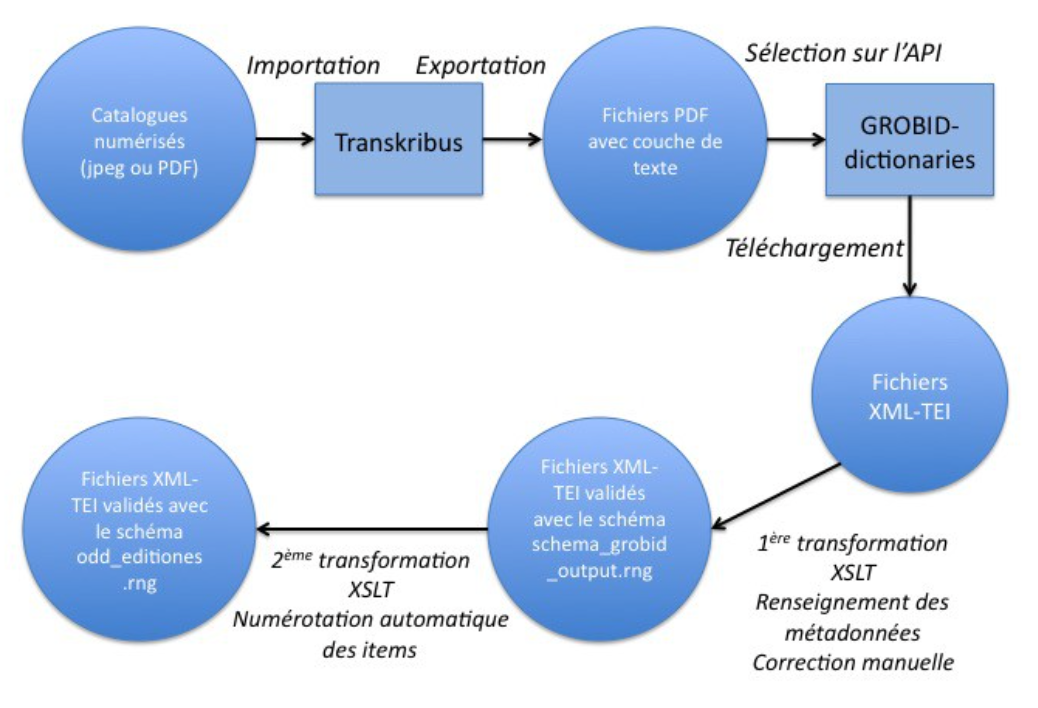
\includegraphics[scale=0.6]{chaine2019}
	\caption{Chaîne de traitement en 2019}
	\label{2019}
\end{figure}


\section{Stage 2020 : systématiser un workflow (Transkribus + Grobid + ALTO)}

En 2020, un nouveau stage en continuité directe avec l'antérieur a été proposé par Béatrice Joyeux-Prunel au sein du projet Artl@s. En contact avec Simon Gabay et l'équipe ALMAnaCH de l'INRIA (responsable de développer le logiciel GROBID), elle a proposée la base de données BasArt et le corpus du projet Artl@s comme nouveaux laboratoires pour approfondir la recherche sur l'encodage automatique de catalogues. Il s'agissait donc de développer un outil déployable au sein d'une équipe de chercheurs avec des compétences numériques limitées, adapté à une déclinaison particulière de catalogue fondamentale pour la recherche en histoire de l'art.

La mission a été assurée par Caroline Corbières, dont le mémoire de fin de stage\footcite{corbieres_du_2020} retrace une série d'expériences techniques qui l'ont mené a développer un \textit{workflow} adapté au traitement de catalogues d'expositions d'art du XIXe et XXe siècle. Il s'agissait de définir des méthodes adaptées à un corpus vaste et en perpétuel développement, avec le travail de Lucie Rondeau du Noyer comme appui pour automatiser l'encodage d'entrées et les verser dans BasArt. Cette chaîne intègre un nouveau type de document, le fichier ALTO, du fait des horizons qu'il ouvre pour l'encodage et l'extraction du texte sur plusieurs étapes.

Le mémoire de Caroline Corbières s'attarde cette fois non pas sur des enjeux historiographiques, mais sur les implications épistémologiques des réalités institutionnelles à l'œuvre dans l'engrenage scientifique. Les intérêts partagés par plusieurs groupes de travail (Artl@s, e-ditiones, ALMAnaCH), les atouts et les limites du travail collaboratif, sont présentés comme les fondements ultimes d'un outil qu'il faut situer dans son contexte de production. La mission a été chargée par ces acteurs d'un caractère expérimental, afin de tester des alternatives de plus en plus efficaces dans l'automatisation de l'encodage de catalogues. Ainsi, l'objectif était double : adapter le workflow de Lucie Rondeau du Noyer au projet Artl@s, et évaluer des données inédites prenant en compte des facteurs nouveaux (notamment l'emphase typographique) pour observer le comportement du logiciel GROBID face à ces nouveaux éléments (\textit{features}).

L'apport fondamental de la mission tourne autour d'une réflexion sur l'encodage des catalogues d'art en TEI, mise en pratique avec le développement d'une ODD qui constitue encore à ce jour le schéma des encodages du corpus. Caroline Corbières a décliné des typologies de catalogues d'exposition puis proposé des balises sémantiquement adaptées à une description générale de ces objet, malgré leur hétérogénéité intrinsèque. Des caractéristiques récurrentes ont été signalées et utilisées pour construire un jeu simple mais (toujours) adapté à tous les catalogues d'exposition traités. 

Elle propose une explication de l'arborescence qu'elle a conçu : la liste des entrées de catalogues est  encodée dans une balise \texttt{<list>}, au sein de laquelle se trouvent toutes les entrées \texttt{<entry>}. Tous les catalogues sont composées de deux parties distinctes relevant de l’exposant et de l’œuvre (à l'exception près des expositions individuelles, qui contiennent généralement une liste simple des œuvres). Une \texttt{<entry>}, numérotée avec un attribut \texttt{@n}, est composée d’une balise \texttt{<desc>} (description), où sont indiquées les informations complémentaires relatives à l’exposant, et d’un ou plusieurs \texttt{<item>} qui correspondent aux œuvres. Dans ces dernières se trouvent le titre et des informations éventuelles. L'exposant possède aussi une balise \texttt{<desc>} est divisée en deux sections :
\begin{itemize}
	\item \texttt{<name>} : nom de l’artiste. Il est possible de différencie nom et prénom avec les balises  \texttt{<surname>} et \texttt{<forename>}
	\item La balise \texttt{<trait>} suivie de \texttt{<p>} regroupe  les informations complémentaires. Il est possible d’ajouter les balises suivantes : \texttt{<birth>}, \texttt{<death>}, \texttt{<residence>}, \texttt{<education>}, \texttt{<affiliation>} et \texttt{<nationality>}.
\end{itemize}

L’\texttt{<item>} (œuvre), numéroté avec un attribut \texttt{@n}, est divisé en trois parties :
\begin{itemize}
	\item \texttt{<num>} : indique le numéro de l’\texttt{<item>} tel qu'il apparaît sur le catalogue
	\item \texttt{<title>} : titre de l’œuvre
	\item \texttt{<desc>} : description de l’œuvre. Il est possible d’encoder les informations suivantes : \texttt{<material>} (technique artistique), \texttt{<dimensions>}, \texttt{<date>}, \texttt{<history>} (provenance), \texttt{<measure>} et \texttt{<note>}
\end{itemize}

La mission a été l'occasion de faire des expériences pour tester des nouvelles conditions techniques dans l'extraction des entrées. La première était l'implémentation prévue du standard XML ALTO sur GROBID, qui a été considérée par les directeurs de stage comme un fichier adapté à une description plus détaillée de la structure typographique des catalogues. En effet, contrairement au format \texttt{.pdf}, \texttt{input} antérieur pour l'OCR, les fichier ALTO permettent d'ajouter des indications sur l'emphase typographique. GROBID-dictionaries s’appuie  pour sa part sur des \textit{features}, c'est à dire la localisation d'éléments récurrents dans la page, pour établir des modèles de reconnaissance des entrées. Elles avaient été utilisées auparavant pour détecter la mise en page du document selon le positionnement spatial du texte et l'utilisation de la ponctuation, de caractères spéciaux ou de retours à la ligne. Avec ALTO, il est possible d'ajouter de nouvelles \textit{features}, telles que l'emphase typographique avec du gras, l'italique ou la taille de la police. Dans le cadre du travail collaboratif complémentaire au stage, Simon Gabay et Ljudmila Petkovic ont entraîné un modèle HTR qui reconnaît les mots en gras et en italique, puis les encode dans des balises \texttt{<b>} et \texttt{<i>} grâce à des scripts python.

Cependant, la publication de la version GROBID capable de prendre des fichiers ALTO en \texttt{input} a été retardé en raison des nombreuses difficultés techniques que cette nouvelle fonctionnalité impliquait. Cette contrainte logistique a imposé de changer la stratégie technique : la solution proposé a été un retour vers le format PDF, depuis l'ALTO, qui contiendrait des indications relatives aux emphases typographiques dans le texte même. Ce passage des fichiers ALTO vers du PDF, nouvelle étape, a été mis en œuvre avec XSL-FO, un vocabulaire XSL qui permet de décrire la mise en page d’un document. Postérieurement, il a été possible d'utiliser la nouvelle version de GROBID, et donc d'évaluer la performance des deux méthodes : l'information typographique a eu un impact positif conséquent dans l'extraction des entrées, et fonctionne mieux sur des documents PDF puisqu'il est beaucoup plus complexe de reconstituer le texte à partir des fichiers ALTO. 

Outre l'amélioration du processus d'extraction, l'enjeu du stage était sa systématisation, c'est à dire la création d'un workflow réutilisable par les membres du projet d’Artl@s. Il est possible d'observer un schéma de cette chaîne de traitement sur la figure \ref{2020}. Avec un fichier \texttt{.pdf} ou \texttt{.jpeg} en entrée, le \textit{workflow} mènera l'utilisateur à produire un encodage TEI ou un tableur CSV en six étapes :
\begin{itemize}
	\item import du catalogue (\texttt{.pdf} ou \texttt{.jpeg})
	\item OCRisation du catalogue et exportation de la transcription dans des fichiers ALTO avec Transkribus
	\item transformation des fichiers ALTO en PDF
	\item encodage automatique avec GROBID-dictionaries
	\item transformation XSL pour produire un document TEI conforme avec l'\texttt{output} de GROBID
	\item transformation éventuelle du fichier TEI en tableur CSV
\end{itemize}
La mission s'est donc achevé avec un \textit{workflow} systématisé. Cependant, certaines limites relatives à son caractère "User Friendly" sont manifestes et signalés par l'autrice même. Si un guide complet avec des captures d'écran accompagne l'utilisateur dans le déploiement des étapes et des technologies concernées, il est virtuellement impossible d'accomplir le travail sans certaines aptitudes numériques intermédiaires. L'emploi du terminal est inévitable : il faut exécuter des scripts python, lancer des entrainements GROBID, accéder à un serveur local, et connaître les commandes \texttt{git}. Par ailleurs, il s'agit d'une chaîne de traitement hachée, impliquant des technologies complexes et des manipulations intermittentes de fichiers à gérer à chaque étape. Ces conditions allaient sous-tendre des nouvelles directions pour les stages à venir, et notamment la volonté de créer un outil au service des chercheurs et des étudiants.


\begin{figure}
	\centering
	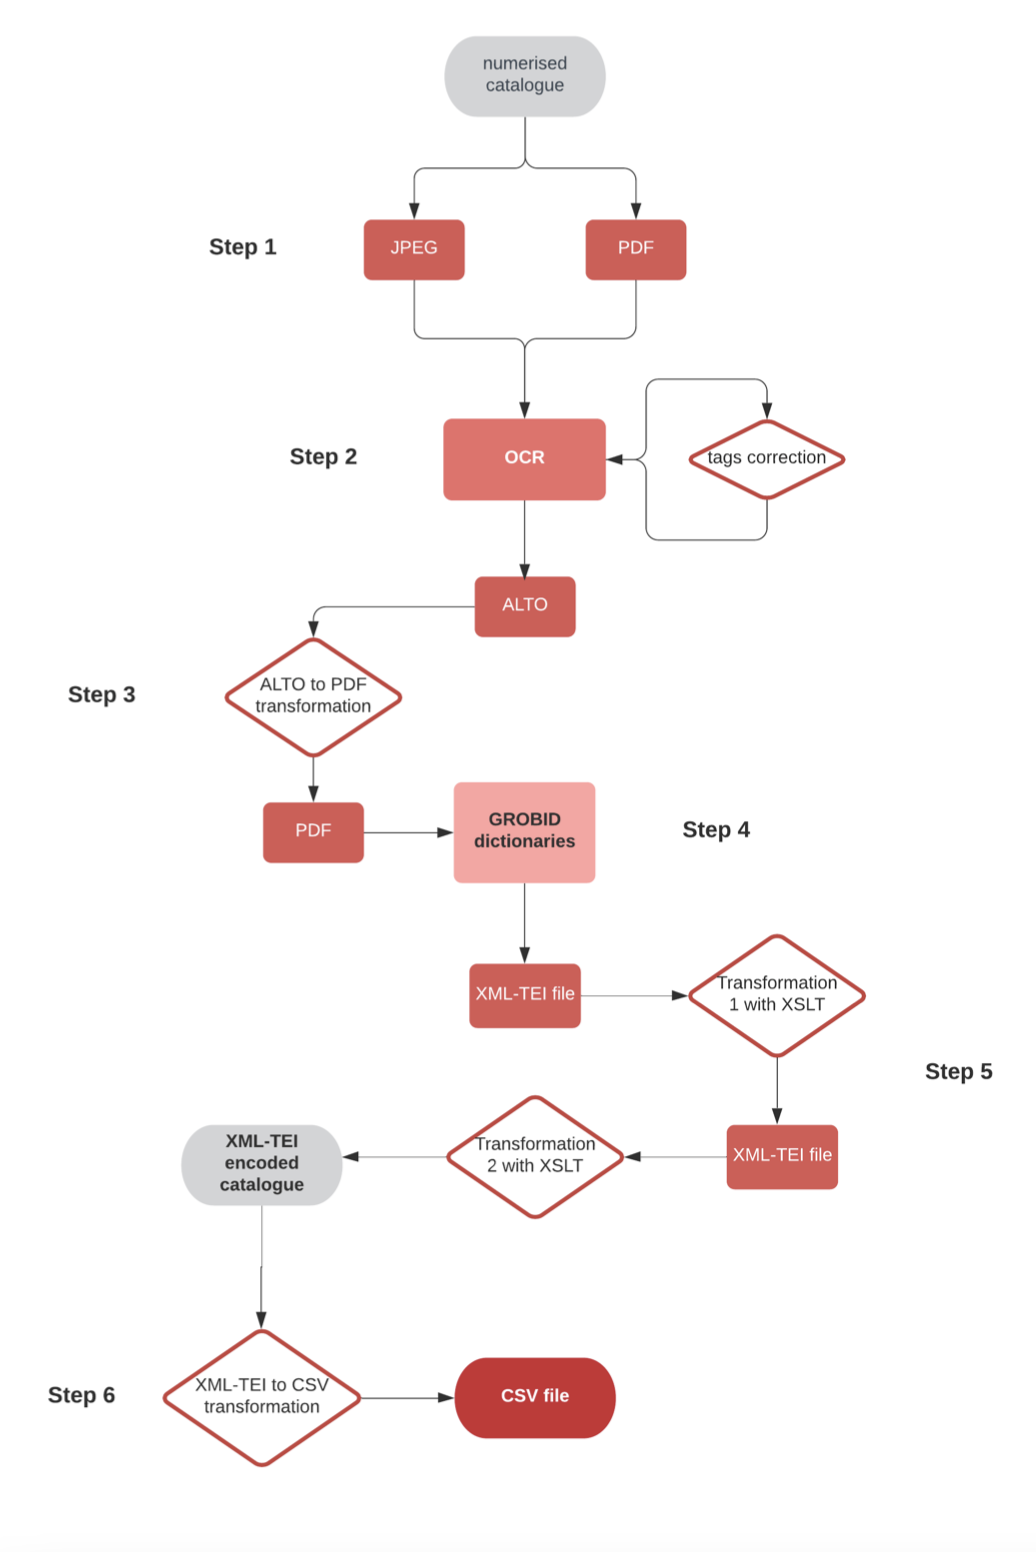
\includegraphics[scale=0.4]{chaine2020}
	\caption{Chaîne de traitement en 2020}
	\label{2020}
\end{figure}



\section{Stage 2021 : migration vers la science ouverte (kraken + python)}
\label{chap:stage2021}

Un deuxième stage a été proposé en 2021 conjointement par Béatrice Joyeux-Prunel et Simon Gabay. Le logiciel Transkribus est devenu payant en 2020, ce qui a mené à repenser dans ses fondements mêmes la chaîne de traitement développée depuis 2019. Le stage a été donc axé autour d'un réflexion sur la science ouverte et a consisté à concrétiser une migration vers des logiciels libres et gratuits. Juliette Janès a mené cette mission en concentrant ces efforts dans l'entrainement de nouveaux modèles de reconnaissance de caractères. Une deuxième étape à consisté à mettre le logiciel GROBID de côté, pour tester un prototype spécifiquement adapté aux traitement de catalogues d'exposition d'art pour la base de données BasArt. Cette section décrira quelques aspects techniques du script produit à cette occasion, pour pouvoir expliquer postérieurement les transformations que qu'il a subi pendant le stage en 2022. 

Le mémoire de fin de stage\footcite{janesCataloguePapierAu2021} de Juliette Janès s'organise autour d'une chronique des transitions opérées, ponctué par une réflexion générale autour des enjeux et des horizons pragmatiques de la science ouverte. En effet, certaines des préconisations fondamentales\footcite{urfist_mediterranee_les_nodate, wilkinson_fair_2016, vanholsbeeck_la_2017} de ce mouvement sont au cœur même du projet Artl@s depuis son inauguration en 2008 : partage de l'information, encouragement de la collaboration scientifique, intégrité et reproductibilité des données et des méthodologies. Béatrice Joyeux-Prunel souhaitait une chaîne de traitement ouverte sans logiciels payants, avec l'objectif spécifique de la rendre reproductible. Le mémoire est axé autour d'un recul critique sur la démarche, avec pour problématique la question pressante de la pertinence d'outils libres mais parfois moins efficaces : "quels sont les apports réels de la restructuration complète d’une chaîne de traitement, pourtant fonctionnelle, dans le but de la rendre intégralement ouverte, libre et gratuite ?". 

La transformation de Transkribus vers un système de services payants a eu un impact global sur la chaîne de traitement, ce qui a été saisi comme une opportunité pour faire évoluer le projet afin de le rendre plus autonome. Il a rapidement été décidé d'utiliser kraken et l'interface eScriptorium, une application web qui permet de visualiser ses commandes avec des fonctionnalités supplémentaires d'édition manuelle des fichiers. Puis l'utilisation même du logiciel GROBID a commencé à poser certains problèmes. Premièrement, l'équipe ALMAnaCH s'est aperçu que les fichiers ALTO produits par kraken sont différents de ceux produits par Transkribus ; il faudrait attendre à ce que GROBID-dictionaries soit compatible avec l'\texttt{output} de kraken. De plus, le développement du logiciel GROBID-dictionaries semblait compromis du fait du départ de son concepteur de l'INRIA, Mohamed Khemakhem. De plus, malgré son efficacité, il s'agit d'un logiciel qu'il faut entrainer pour chaque catalogue, ce qui complique l'usage du pipeline pour des personnes sans les aptitudes techniques requises. L'idée d'un prototype de script d'extraction des entrées, spécifique aux catalogues de la base de données BasArt, est alors apparue comme un projet souhaitable et envisageable.

La mission s'est concentré sur la migration des jeux de données d’entrainement des modèles d’OCR depuis Transkribus vers kraken. Il s'agit d'un travail complexe qui a été mené de manière très satisfaisante. Une transcription automatique fonctionne avec des modèles entraînés sur des jeux de données particuliers et Transkribus ne permet pas d’extraire ces éléments pour les injecter dans un nouveau logiciel. Il fallait donc procéder à une compagne complète de réentraînement des modèles, avec des données issues des corpus des projets Artl@s et Katabase. Cela a impliqué des efforts considérables, mais plusieurs atouts sont manifestes : il est possible de contrôler et d'améliorer l'OCR, ainsi que de connaître dans son ensemble le fonctionnement du processus de transcription. 
Il a fallu injecteur dans eScriptorium des fichiers de transcription en \texttt{output} de transkribus, adaptés au nouveau logiciel avec des feuilles de transformation XSL. Deuxièmement, des modèles de segmentation et de reconnaissance de caractères ont été entraînés avec ces données. En effet, kraken est un logiciel qui fonctionne sur deux étapes : le \textit{layout analysis} (analyse de mise en page) puis la reconnaissance de caractères à proprement parler. l'OCR repère d'abord la structure de la page et les éléments qui la forment. Il reconnait aussi les lignes, qui sont matérialisées de deux manières : en tant que \textit{baseline}, ligne suivant le bas du texte, et en tant que masque, qui couvre l'ensemble des caractères de la ligne. Postérieurement, un modèle de reconnaissances de caractères est appliqué.

L'OCR est basé sur du \textit{machine learning}, branche de l'intelligence artificielle qui s'occupe de la création de modèles et d'algorithmes à partir de corpus de données. Il faut fournir des données suffisantes pour que la machine les analyse et apprenne à reconnaitre dans l'image des structures de pixels à associer avec des caractères encodés. Il s'agit concrêtement de fournir au logiciel des images de page accompagnées de leurs transcription ALTO, ce qui a été fait avec un corpus de 500 pages de catalogues d'exposition (150) et de ventes de manuscrits autographes (350) des XIXe et XXe siècles. Ces données connues et vérifiées par la machine constituent le \textit{grountruth} ("vérité de terrain"). Contrairement à la grande majorité des logiciels OCR, kraken permet la récupération des modèles, ce qui rend possible le partage et la conservation des entraînements. 

L'autre volet du stage a consisté à développer un prototype de script python pour extraire les données de l'\texttt{output} d'eScriptorium et les structurer en tant que fichiers TEI conformes à l'ODD définie par Caroline Corbières en 2020. Cet outil, placé au centre du stage en 2022, avait été alors conçu comme un instrument expérimental ne pouvant fonctionner qu'avec une sélection restreinte de catalogues. Nous décrirons deux éléments constitutifs de ce programme qui on fait l'objet d'améliorations qui seront présentées postérieurement dans notre mémoire. 

Le premier est l'implémentation d'expressions régulières utilisées pour déterminer avec quelles balises encoder chaque ligne. Elles sont censées permettre à la machine de comprendre si la ligne signale un auteur, des œuvres, des informations complémentaires, ou bien des combinaisons des éléments précédents. Un seul fichier python réunissait une série de regex simples adaptées à des cas différents, et l'utilisateur était censé le manipuler pour activer uniquement celles dont il avait besoin. Cela impliquait, pour chaque exécution du script, de vérifier quelle expression régulière est adaptée au catalogue courant, et d'intervenir sur le code.


Deuxièmement, face aux limites techniques impliquées par la perte de l'encodage automatique offert par GROBID-dictionaries, il a été nécessaire de réfléchir à de nouvelles méthodes pour l'extraction textuelle des transcriptions. Celle-ci a mené à définir une typologie de catalogues d'exposition d'art nécessitant des traitements différents et adaptés à chaque cas (voir figure \ref{typologie}). Des commandes spéciales ont été créées pour que l'utilisateur indique le type après une analyse visuelle de la structure des catalogues :\\
\begin{itemize}
	\item Simple : pour les catalogues ayant des entrées de type 1.A.
	\item Double : pour les catalogues ayant des entrées de type 1.B
	\item Triple : pour les catalogues ayant des entrées de type 1.B et des lignes d'informations supplémentaires
	\item Nulle : pour les catalogues ayant des entrées de type 1.C
\end{itemize}

Voici le schéma de la commande pour lancer le script :

\begin{normalsize}
	\begin{minted}{bash}
		python3 run.py input titre type titre.xml -v -st
	\end{minted}
\end{normalsize}

Voici une explication de chaque élément :

\begin{itemize}
	\item \texttt{python3} : lance le langage de programmation python3
	\item \texttt{run.py} : exécute le fichier python principal 
	\item \texttt{input} : chemin vers les fichiers ALTO contenant les transcriptions
	\item \texttt{titre} : titre pour les ID TEI
	\item \texttt{type} : type de catalogue selon la typologie définie
	\item \texttt{titre.xml} : titre pour le fichier TEI
	\item \texttt{-v} : option de vérification de la structure des fichiers ALTO
	\item \texttt{-st} : option de segmentation et transcription automatique avec kraken et des images en \texttt{input} 
\end{itemize} 

Pour ce prototype, uniquement des catalogues de type "simple" ont été traités, c'est à dire que chaque ligne ne pouvait correspondre qu'à un seul type d'information bien distincte : exposant, informations, œuvres. Cela a permis d'encoder six catalogues préalablement transcrits, mais le script reste inutilisable pour le reste du corpus. Plusieurs problèmes sont à signaler : les indications d'erreurs sont très limitées, les commandes redondantes et compliquées, et l'exécution implique une analyse humaine préalable du catalogue fourni. Le script fonctionnant rarement, et son exécution nécessitant des ajustements chronophages, il est extrêmement difficile de comprendre l'origine des divers problèmes. De plus, les corrections manuelles doivent être réalisées sur les fichiers ALTO en \texttt{input} et sur le fichier TEI en \texttt{output}, ce qui peut être très difficile pour des débutants. Juliette Janès signale que, contrairement à la vocation des chaînes de traitement antérieures, cet outil complique à l'extrême, voir interdit la prise en main par des néophytes. Le script propose pourtant une méthode intelligente et  prometteuse, développée à partir de rien, qui a retenu l'intérêt des directeurs du stage pour la mission à venir. 


\begin{figure}
	\centering
	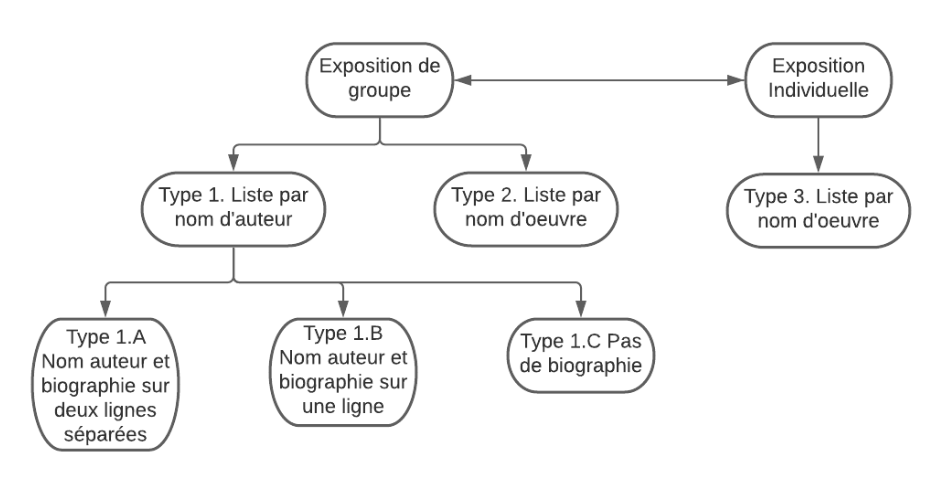
\includegraphics[scale=0.6]{typologie_JJanes}
	\caption{Typologie des catalogues pour le programme python en 2021}
	\label{typologie}
\end{figure}
\begin{figure}
	\centering
	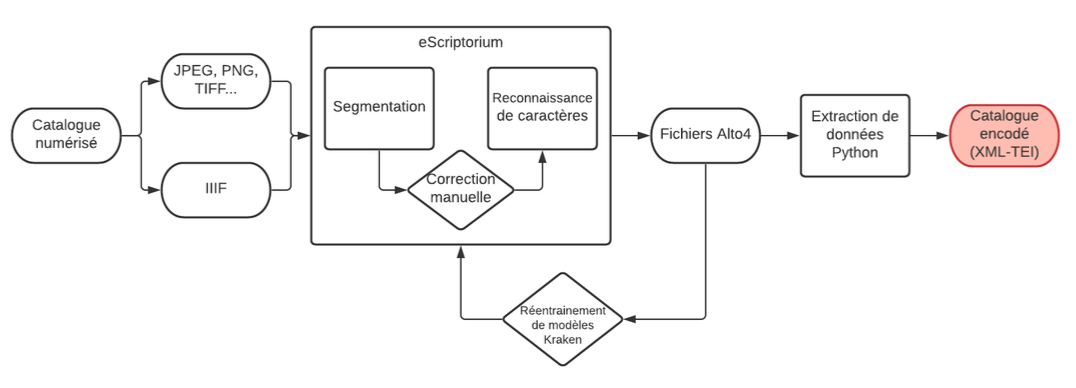
\includegraphics[scale=0.6]{chaine2021}
	\caption{Chaîne de traitement en 2021}
	\label{2021}
\end{figure}





	\chapter{Stage 2022 : produire efficacement des données ou enseigner correctement ?}
Ce chapitre ne présente pas un bilan rétrospectif du stage en 2022, qui est l'objet général du présent mémoire. Il tente plutôt, suite à la chronique des missions entre 2019 et 2021, de positionner dans leur continuité l'évolution des enjeux scientifiques, les objectifs des directeurs, ainsi que les problèmes techniques qui ont été affrontés.

Suite à trois stages proposant des explorations complémentaires mais aussi parfois des ruptures radicales, une nouvelle mission pouvait ête envisagée avec un horizon pragmatique clair. Les chaînes de traitement possibles, améliorées techniquement et presque totalement conformes aux préconisations épistémologiques et éthiques de la science ouverte, offraient une plateforme solide pour abandonner le terrain prospectif de l'expérimentation. Béatrice Joyeux-Prunel et Simon Gabay souhaitaient d'une part un produit scientifiquement productif, de l'autre un outil pédagogique fiable et abordable pour introduire des étudiants en sciences humaines aux humanités numériques. L'enjeu était de parfaire le pipeline en même temps que de le rendre accessible, dans un contexte ou les méthodes employées en vue d'améliorations techniques avaient fini par rendre l'outil de plus en plus difficile à prendre en main. En découlent deux directions tantôt complémentaires, tantôt contradictoires : produire efficacement des données ou enseigner consciencieusement les humanités numériques ? 

Nous présenterons la mission dans le contexte des problématiques non résolues par les stages antérieurs, ainsi que dans le cadre de perspectives techniques et scientifiques solides que ces missions ont contribué à construire. Nous évoquerons des directions abandonnées, du fait de la consolidation du sens donné à notre mission, mais aussi du fait de contraintes logistiques qui ont impliqué de mettre de côté certains objectifs. Finalement, nous proposerons une synthèse des contributions techniques effectuées la mission durant, au regard des problèmes suscités au cours des expériences antérieures.


\section{Positionnement de la mission}

Le stage 2022 s'ancre pleinement dans une continuité avec les missions précédentes, puisqu'il a consisté à reprendre des outils construits antérieurement et présentant des nombreuses problématiques techniques. L'objectif fondamental était de parfaire un pipeline et le rendre pour la première fois véritablement utilisable par des groupes d'utilisateurs (étudiants et chercheurs associés) contribuant à produire des données pour la base BasArt. 

Il peut être donc conçu comme un prolongement direct du stage de Juliette Janès, qui a réalisé une migration très satisfaisante vers des instruments conformes à la science ouverte, a entamé un travail approfondi d'entraînement de modèles de reconnissance sur kraken, et s'est aventuré à proposer un prototype ambitieux pour l'extraction des entrées de catalogue. Afin de constituer une chaîne de traitement authentiquement abordable par des néophytes, il est apparu comme prioritaire de travailler principalement sur cette dernière étape du pipeline. Si cela posait le défi technique de développer un script qui dépasse le statut expérimental, l'horizon envisagé pouvait être considéré comme un nouveau cap franchi pour le projet. Le livrable attendu et réalisé est un pipeline consistant en deux étapes  simples à mettre en oeuvre : transcription des catalogues sur l'interface eScriptorium puis exécution d'un script d'extraction des entrées à travers d'un notebook Jupyter.

Outre les limites techniques que l'on retrouve sur le script python développé en 2021, le problème général à résoudre était de remettre au centre du travail une vocation initiale évacuée au fil des stages. En effet, les mémoire successifs prennent soin de noter les difficultés à mettre en place des chaînes de traitement "user friendly". Il est possible d'aller au delà et de dire qu'aucun traitement "automatique" n'a été véritablement atteint (le terme est systématiquement employé pour qualifier les productions). En effet, les logiciels utilisés nécessitent des traitements intermédiaires des fichiers en \texttt{input} et en \texttt{output}, et il a toujours été nécessaire de faire usage de commandes sur un terminal. Plus est, la transition opérée vers des outils de la science ouverte à bien ouvert les horizons désirés, mais a impliqué de complexifier la chaîne de traitement et de la rendre absolument inabordable par des débutants. Le pipeline actuel se revendique comme semi-automatique, et permet un déploiement immédiat (notamment à l'aide de nombreux exemples qui nécessitent pas de travail préalable sur eScriptorium), en accompagnant tout au long du processus les utilisateurs débutants.

\section{Projets exclus}

Plusieurs projets envisagés avant ou pendant le stage on été mis de côté, des fois pour des raisons de cohérence technique, mais aussi du fait de contraintes temporelles ; ils peuvent être considérés en ce sens comme des ambitions non satisfaites. Cette section décrit les principaux projets abandonnés en cours de route afin de donner plus d'éléments sur la signification de la mission et de suggérer des améliorations futures. 

Premièrement, Simon Gabay avait pensé à développer le script python en confrontant deux méthodes : l'une prolongerait l'extraction commencée par Juliette Janès, qui se base sur la reconnaissance des lignes de texte avec des expressions régulières, et qui inclue une étape préalable qui repère et utilise les zones de la page. Ces zones, conformes au standard de nommage des régions de l'ontologie Segmonto (voir chapitre 6.2.2), sont saisies par l'utilisateur sur l'interface eScriptorium. Il s'agit de signaler directement quel est l'espace occupé par une entrée de catalogue, ce qui a une implication majeure : le script ne peut comprendre que des fichires ALTO et leur manière d'indiquer ces informations. En conséquence, les seuls fichiers traitables par le programme proviennent de transcriptions contenant des segmentations conformes à l'ontologie Segmonto.

Cela ne pose pas de problème majeur dans le cadre de la vocation pédagogique du pipeline, qui peut ainsi présenter ces trois technologies des humanités numériques à des étudiants. Cependant, l'idée était de créer un deuxième script qui ne prenne pas en compte les régions de la page, et qui fonctionnerait exclusivement avec des expressions régulières. Cela aurait permis, en plus des fichiers ALTO, d'insérer des fichiers de texte brut et \texttt{.pdf}. L'enjeu majeur aurait été alors de savoir s'il était possible qu'un tel programme soit efficace, puisqu'il permettrait alors un enrichissement exponentiel des données de BasArt. Il est donc intéressant d'envisager un tel instrument, qui permettrait de rendre le pipeline plus efficient et automatique, ou bien de confirmer la pertinence d'un travail avec la segmentation des zones. Faute de temps, il a été décidé de concentrer les efforts sur le premier script, afin de le rendre pleinement fonctionnel, puisque ses résultats commençaient à être très satisfaisants et qu'il a été jugé plus important de préparer un instrument pédagogique solide pour la rentrée 2023.

Un autre chemin sans issue a été l'exploration du logiciel de reconnaissance de caractères kraken. Celui-ci avait été mis de côté dès le début dans le cadre du stage, mais son installation en local pour apprendre les manipulations fondamentales paraissait pertinente en vue d'expériences qui pourraient avoir eu lieu en fin de stage. Cependant, l'installation a été extrêmement problématique et nous a fait perdre plusieurs jours de travail, ce qui a rendu impossible de revenir postérieurement sur le logiciel. Il s'agissait d'un conflit de dépendances de librairies python sur MacOS intel 2020 actuellement non résolu, qui a pu être détecté grâce à l'aide de Ben Kiessling, l'ingénieur qui a développé kraken. L'expérience n'était tout de même pas inutile, puisqu'elle nous a fourni un simulacre de travail collaboratif dans le débuggage de logiciels open source\footnote{L'Issue et sa résolution peuvent être consultés ici : \url{https://github.com/mittagessen/kraken/issues/348}}. 

Une deuxième problématique liée à kraken se trouve dans le script python même, et constitue le seul problème technique à ne pas avoir été résolu pendant la mission. Juliette Janès à intégrée une commande \texttt{-st} optionnelle foncièrement expérimentale (puisque non fonctionnelle), qui permettrait de mettre en \texttt{input} des images et d'obtenir leur segmentation et transcription automatiques directement à travers du script. Si les problèmes purement techniques du code on été résolus, cette fonction est inutilisable, car la segmentation automatique n'utilise pas les régions Segmonto nécessaires pour que le script marche correctement. De plus, à ce jour, les modèles de segmentation automatique des zones de la page ne donnent pas de résultats satisfaisants, et notre pipeline implique que l'utilisateur saisisse manuellement ces zones sur l'interface eScriptorium. Ces difficultés pourraient être résolues dans un futur proche : Segmonto est un standard qui se généralise (et Simon Gabay réfléchi à son intégration dans FoNDUE, l'implémentation locale d'eScriptorium de l'Université de Genève) ; deuxièmement, le développement de modèles de segmentation efficients est au centre de nouveaux stages qu'il dirige. De telles avancées pourraient mener à créer un script python véritablement automatique, nécessitant uniquement des corrections sur les fichiers en \texttt{output} (TEI ou CSV). 

Nous pouvons mentionner finalement un outil imaginé par Juliette Janès et mis de côté avant le début même du stage 2022. Elle suggérait de créer à partir de son prototype une interface Web dédiée, qui faciliterait l'utilisation du programme python avec des fonctionnalités spécifiques. La proposition était intéressante mais demandait un investissement important de travail. L'idée d'un notebook a paru alors beaucoup plus adaptée, puisqu'il s'agit d'un outil facile à construire et utiliser, déployé au sein même d'un navigateur Web. Une interface dédiée aurait permis tout de même d'aller très loin dans la personnalisation de des outils, et d'implémenter par exemple un instrument pour tester des expressions régulières, ainsi qu'une base d'images de catalogue pour aider l'utilisateur à identifier le type de son document. Cependant, ces fonctionnalités s'avèrent actuellement inutiles, puisque dans son état actuel le script détecte automatiquement le type de catalogue et possède une implémentation regex solide, le tout pouvant être lancé depuis Jupyter Notebook.




\section{Le choix d'un pipeline échelonné et pédagogique}

De manière globale, les projets exclus ont été mis de côté au profit d'un même objectif : développer un pipeline à vocation pédagogique. Béatrice Joyeux-Prunel souhaite que le travail de contribution pour BasArt soit lié à la formation d'étudiants suivant des cours d'introduction aux humanités numériques à l'Université de Genève. Il s'agit d'étudiants réalisant des diplômes en science humaines au niveau bachelor et master, ainsi que du certificat de spécialisation en humanités numériques pour masterants, doctorants et post-doctorants. 

Cela permet de solidariser plusieurs missions, telles que la production de données pour la recherche en histoire de l'art et la transmission d'une culture numérique plus solide. Ainsi, le caractère semi-automatique du pipeline devient souhaitable, puisqu'il implique de présenter et de prendre en main des outils ouverts fondamentaux dans le domaine des humanités numériques : OCR (eScriptorium et kraken), python, CSV, et les standards XML TEI et ALTO. Au delà, la méthode étant libre et le code reproductible, son enseignement contribue à la pérennisation du projet, qui peut être récupéré et adapté à de nouveaux usages. 

Contrairement à ce qui avait été envisagé lors des stages antérieurs, l'enjeu n'est plus de contourner des lacunes en culture numérique avec un outil automatique, mais de rendre possible l'acquisition d'une autonomie technique fondamentale pour de futurs chercheurs\footcite{debouyEnseignerHumanitesNumeriques2020}. Il n'y a pas de préalables nécessaires, mais il s'agit de développer des aptitudes et non pas de "bypasser" des obstacles. 

Au delà, l'accessibilité peut rendre l'outil efficace, non plus sur le plan purement technique, mais à travers d'une utilisation aisée et donc généralisable. Des groupes d'étudiants vont en faire usage, et la production de données pourra être considéré comme un marqueur pour évaluer le pipeline et mettre en lumière des améliorations nécessaires. 









\chapter{Résultats du travail}

Ce chapitre présente le résultats du travail sur le script extractionCatalogs dans le cadre du stage, de sa poursuite des missions précédentes, et de son insertion dans le projet Artl@s. Il ne fait donc pas une présentation exclusivement technique, et ne fournit pas des explications sur le fonctionnement global et linéaire du pipeline. Pour une approche détaillée, le lecteur doit consulter la partie 3 du présent mémoire. Il peut être préférable de le faire avant dans le cas où le lecteur ne soit pas familiarisé avec les technologies et logiciels évoquées : eScriptorium, kraken, python, XML TEI et ALTO. 

Une liste simplifiée indiquant l'ensemble de améliorations apportées au prototype de 2021 de Juliette Janès peut être consultée dans l'annexe A. Celle-ci permet de retracer concrètement les problèmes suscités par le scritp et les transformations opérées. 

Le pipeline comporte deux étapes fondamentales (une liste plus détaillée peut être consultée dans l'introduction de la partie 3) : 

\begin{enumerate}
	\item L'utilisation d'eScriptorium, une interface web qui permet d'utiliser le logiciel d'OCR kraken et qui offre des fonctionnalités suppémentaire d'édition des documents produits. 
	\begin{itemize}
		\item \texttt{input} : catalogue numérisé (manifeste \texttt{iiif} ou \texttt{.jpg}, \texttt{.png}, \texttt{.pdf}, etc.)
		\item Segmentation automatique des lignes
		\item Transcription automatique avec un modèle dédié
		\item Correction manuelles sur l'interface même
		\item Segmentation manuelle sur l'interface même : l'utilisateur doit saisir et nommer les régions sémantiques de la page (entrées, etc.) selon l'ontologie Segmonto	
		\item \texttt{output} : fichiers XML ALTO4 (encodage du texte et de son positionnement spatial dans les zones de la page)
	\end{itemize}
	
	\item L'utilisation du programme extractionCatalogs, qui traite les données produites lors de l'étape antérieure, pour produire les fichiers souhaités (restructurations ALTO, encodage en XML-TEI et tableurs CSV)
	\begin{itemize}
		\item \texttt{input} : fichiers XML ALTO4 produits sur eScriptorium
		\item lancement du script avec la commande suivante :
		\begin{normalsize}
			\begin{minted}{bash}
!python3 run.py   chemin_input   chemin_output   nom_du_catalogue
			\end{minted}
		\end{normalsize}
		\item le script python 3 traite automatiquement les fichiers en entrée. Pour chaque fichier ALTO (qui comporte l'encodage d'une page individuelle de catalogue), il analyse le document ligne par ligne pour reconstituer le catalogue, entrée par entrée.
		\item \texttt{output} : fichier XML-TEI contenant l'encodage des entrées du catalogue.
		\item \texttt{output} : tableurs CSV produits à partir du fichier TEI. Ceux-ci permettent une lecture humaine et l'injection des données dans la base BasArt
		\item \texttt{output} : fichier \texttt{.txt} indiquant des problèmes d'extraction, pour que l'utilisateur/utilisatrice puisse faire des corrections manuelles.
	\end{itemize}
\end{enumerate}


\section{Problèmes techniques affrontés pendant la mission}

Cette section décrit quelques problèmes techniques affrontés lors de la prise en main du prototype python. Les problèmes d'ordre logistique ou relatifs à des projets sans aboutissement sont décrits dans le chapitre 2.2. cette prise en main a été hasardeuse, du fait de sa complexité technique mais aussi de ses dysfonctionnements. Un premier lancement fonctionnel du programme n'a été possible qu'après certaines corrections sur le code. Le manque de commentaires ou de noms sémantiquement clairs pour les variables et les fonctions ont également ralenti la compréhension du processus. Il a fallu l'appréhender avec la seule lecture des fichiers python \texttt{.py}, faute de résultats satisfaisants en \texttt{output}. Voici une liste non exhaustive de problèmes pour le lancement initial :
\begin{itemize}
	\item Impossibilité de traiter des dossiers contenant des fichiers autres que ALTO (par exemple, leurs images associées)
	\item Impossibilité de traiter des dossiers avec des fichiers cachés
	\item Sur MacOs, impossibilité de traiter des dossiers avec des fichiers \texttt{.DS\_Store}. Ces fichiers ne peuvent pas être effacés manuellement.
	\item \texttt Fonctions parsemés de \textit{bugs} et arrêt immédiat du script
	\item Requêtes xpath avec des erreurs (entre autres, non adaptées à la migration vers l'ontologie Segmonto)
	\item \texttt{output} directement déposé dans le dossier du script. L'exécution du script écrase les \texttt{output} antérieurs
	\item  lecture désordonnée des fichiers, produisant des fichiers TEI désordonnés et non conformes à l'ODD
\end{itemize}

Les premières étapes de travail ont consisté à restructurer l'ensemble des dossiers du script, à renommer les fonctions et les variables pour les doter de signification sémantique, à commenter de manière prolifique et systématique l'ensemble du script, et à organiser un \texttt{output} clair dans un dossier spécifique. Il a également fallu corriger le teiHeader produit, pour lequel un gabarit à été créé afin de permettre que d'autres projets utilisent le script. L'extraction impliquait de nombreuses erreurs de conformité à l'ODD, qui n'avaient pas été prévues et qui ont pu être réglées sans toucher au schéma : intégration d'items "bis" (répétition des numéros), reconstitutions d'oeuvres ou d'items sur plusieurs lignes, répétition ou erreurs typographiques dans les catalogues, etc.

Cela a permis que le script fonctionne pour des catalogues de tpye "simple" (les seuls traités par Juliette Janès). Ainsi, il a été possible de commencer à travailler sur un script qui puisse traiter correctement tous les catalogues, qui n'étaient pas reconnus du fait de nombreux \textit{bugs} dans le code. Cela a mené, progressivement, à développer des fonctions capables de reconnaître le type de catalogue en \texttt{input} et à adapter leur traitement en fonction des nécessitées. 

Des discussions avec Frédérine Pradier, étudiante du certificat en humanités numériques travaillant sur des catalogues pictorialistes de la fin du XIXe siècle, ont permis d'avoir les retours d'une utilisatrice du prototype de 2021. Si elle a réussi à adapter légèrement le script à son projet, elle a aussi décrit le \textit{workflow} comme défaillant et entravé. Elle a mentionné des problèmes tels que la difficulté des commandes, les problèmes de numérotation automatique, la non conformité TEI, la non intégration des zones Segmonto \texttt{CustomZone:entryEnd}, et la difficulté à comprendre et indiquer le type de catalogue. Par ailleurs l'implémentation d'expressions régulières imposait de les injecter directement dans le code, ce qui était particulièrement difficile à mettre en œuvre. L'encodage de son corpus à donc impliqué une prise en main lente de l'outil, à quoi s'est ajouté la nécessité de corriger manuellement des \texttt{output} décevants : problèmes avec les regex ou des entrées particulières, non conformité TEI, etc. La continuité des échanges à permis de comprendre les nécessités d'une utilisatrice modèle et nous a mené à régler un a un les problèmes évoqués. Actuellement, le script extractionCatalogs a des résultats très satisfaisants sur les six catalogues du corpus pictorialiste transcrit par Frédérine Pradier. 

Un dernier problème majeur du premier script qu'il est important de mentionner est le traitement défaillant des fichiers ALTO en \texttt{input} tout au long du programme. Le script n'était pas capable de traiter des fichiers ALTO contenant des balises \texttt{TextBlock} vides, qui résultent de fausses manipulations récurrentes dans la segmentation manuelle sur eScriptorium. Aussi, Le premier script était doté d'une commande optionnelle \texttt{-v} censée activer une vérification de la conformité des fichiers ALTO, mais celle-ci comportait des erreurs qui arrêtaient directement le programme. Par aileurs, la propre sortie d'eScriptorium posait des problèmes, puisque l'imbrication des éléments dépend de l'ordre de saisie des zones par l'utilisateur. Le script n'est pas adapté à la multiplicité des cas possibles, ce qui avait pour résultat que seulement 6 catalogues dans un corpus de 37 transcriptions soient traitables. Cette particularité des fichiers ALTO en \texttt{output} d'eScriptorium n'était pas connue de Simon Gabay et il m'a fallu invertir des efforts conséquents pour comprendre la situation. Une discussion avec mes directeurs de stage a mené a déterminer qu'une fonction de restructuration pourrait avoir un intérêt qui dépasserait largement le projet Artl@s.  

Nous avons donc traité un à un les problèmes : premièrement, le nouveau script ignore les régions vides de la transcription ALTO, ce qui permet de ne pas générer des entrées vides qui nuisent à la conformité et à la structure de l'\texttt{output} TEI (la numérotation résultait inexacte). Deuxièmement, la commande optionnelle \texttt{-v} a été corrigée et intégrée au script comme étape constitutive et non optionnelle pour produire des informations utiles sur les documents en \texttt{input}.

Par ailleurs, nous avons créé une fonction pour corriger les fichiers ALTO en \texttt{output} d'eScriptorium, puisque l'imbrication des éléments dépend de l'ordre de saisie des zones par l'utilisateur et non pas d'une hiérarchie établie selon le degré de précision par rapport au texte. Cette fonction calcule la position des lignes et des zones, et réordonne l'imbrication les éléments (à la manière d'une poupée russe) pour que le script puisse traiter toutes les transcriptions. Cela a rendu possible de traiter les 37 catalogues du script  (pour plus de détails, veuillez consulter la section 4.4 de la liste intégrée au chapitre 6.2).



\section{Un instrument efficace et éloquent}

Bien au delà de la correction de problèmes techniques, la mission a consisté à doter le script extractionCatalogs de fonctions lui permettant de traiter de manière satisfaisante des catalogues d'exposition d'art pouvant comporter des structures assez différentes. L'enjeu a été de créer un outil nécessitant le moins d'indications possibles, et en mesure de donner des retours constructifs en cas de problèmes. Le programme est censé être suffisamment solide pour qu'il n'y ait pas à faire d'interventions sur le code, qui est pour sa part profusément documenté afin de servir à des fins pédagogiques. 

Cette section explique certains aspects du fonctionnement antérieur du script qui, sans constituer des erreurs, imposaient des contraintes à dépasser. La commande originale du script demandait, en plus des deux commandes d'exécution python, quatre commandes (dont \texttt{type} nécessitant une analyse visuelle préalable du catalogue) et deux options (non fonctionnelles) : 
\begin{normalsize}
	\begin{minted}{bash}
python3 run.py input titre type titre.xml -v -st
	\end{minted}
\end{normalsize}

La nouvelle commande, simplifiée, prend uniquement trois indications : le chemin d'entrée, le chemin de sortie souhaité et le titre à donner : 
\begin{normalsize}
	\begin{minted}{bash}
python3 run.py input output titre
	\end{minted}
\end{normalsize}


Cette commande permet d'exposer plusieurs améliorations fondamentales. Sa simplicité facilite un prise en main immédiate, appuyée par la présence d'exemples de fichiers ALTO dans les dossiers \texttt{/exemple} du script. Part ailleurs, toutes les contraintes relatives aux chemins sont prises en compte : le dossier en \texttt{input} peut contenir des fichiers autres que ALTO, l'on peut choisir le chemin pour l'\texttt{output}, lequel est clairement organisé, et il est possible mais non obligatoire d'indiquer la terminaison \texttt{.xml} dans le titre du catalogue (avant, il fallait indiquer les deux, avec deux commandes différentes). D'ailleurs, si le titre se termine par \texttt{.csv}, le script va produire immédiatement un tableur CSV si un fichier TEI existe déjà, ce qui permet de faire des corrections directement sur lui et d'avoir un CSV en retour sans l'écraser. 

Une avancée particulièrement importante est que l'indication du type du catalogue selon la typologie définie par Juliette Janès n'est plus nécessaire. Elle existe toujours au sein du script et permet divers traitements, raison pour laquelle elle constitue un apport fondamental. Mais l'automatisation de la reconnaissance permet un usage extrêmement simplifié du script. En effet, il fallait antérieurement vérifier la structure des entrées puis déterminer son type selon un typologie sémantiquement confuse : "Nulle", "Simple", "Triple", "Dougle" (voir figure 1.3 du chapitre 1.3).

L'autre partie nécessitant des interventions manuelles était l'implémentation d'expressions régulières. Nous avons développé des regex longues et solides adaptées à des cas très variés issues de la totalité des catalogues du corpus (voir chapitre 6.3). Ainsi, aucune intervention n'est requise sur le code pour pouvoir exécuter le programme.

Afin de mieux gérer les erreurs attendues ou possibles, le script est également doté de fonctions de vérification et imprime de nombreux messages d'erreur permettant à l'utilisateur de localiser rapidement des problèmes spécifiques : entrées non intégrées, problèmes de conformité TEI, ALTO ou Segmonto, problèmes dans la production des fichiers en \texttt{output}. Une liste complète des messages d'erreur peut-être consultée dans l'annexe D du mémoire. À titre d'exemple, c'est grâce à ces messages que nous avons pu comprendre que les fichiers ALTO en \texttt{output} d'eScriptorium comportaient des problèmes d'imbrication. Ces messages, limités au cadre du projet Artl@s, devraient suffire pour faire les corrections nécessaires à toute extraction. Par ailleurs, ces corrections sont facilitées par un fichier de texte brut indiquant toutes les lignes qui n'ont pas été extraites. Nous avons ajouté des indications sur leur nature et sur leur localisation dans l'encodage afin de faciliter la tâche.

Il est important de mentionner que le script est doté d'une sortie claire et concise sur le processus, imprimée sur le terminal sous la forme d'un récapitulatif général de l'extraction. Hormis une liste indentée et visuellement structurée du catalogue dans son ensemble, l'utilisateur obtient un résumé indiquant le nombre d'entrées, d'exposants et d'œuvres extraits.

Finalement, une étape supplémentaire a été ajouté à la chaîne de traitement : la production de deux tableurs CSV, l'un pour lecture humaine, l'autre conçu pour être injecté dans la base BasArt. Ainsi, le pipeline est simplifié en deux grandes étapes, et le script peut être lancé depuis un notebook Jupyter qui accompagne l'utilisateur dans tout le processus. Il n'est plus nécessaire de faire des manipulations intermédiaires entre ces deux étapes (autre que déposer les fichiers produits par eScriptorieum dans un dossier), et l'utilisateur peut être sûr d'obtenir dans tous les cas un \texttt{output} utile, qui explicite des problèmes dans les cas où une extraction ne serait pas possible. L'accompagnement de l'utilisateur, ajouté à l'accomplissement d'un progamme plus performant, devrait permettre une démultiplication des catalogues traitables. Plusieurs corpus seront proposées aux premiers étudiants qui travailleront avec ce pipeline, dont des manifestes \texttt{iiif} de catalogues sur Gallica, des numérisations conservées par l'Université de Pittsburgh, et un corpus du musée d'art et d'histoire de Genève. 


\section{Améliorations possibles}

La mission s'est terminée avec un livrable utilisable dans un cadre pédagogique. Cependant, ses limites manifestes nous permettent de suggérer des améliorations possibles.  

Premièrement, il faut implémenter le traitement de catalogues d'expositions monographiques. Le seul catalogue de ce type dans le corpus\footcite{castagnaryExpositionOeuvresGustave1882} donne en effet un \texttt{output} défaillant, puisque chaque entrée indique le titre de la première œuvre comme un nom d'auteur. Signalons tout de même que l'extraction est réalisée correctement du début à la fin : il s'agit donc d'une manipulation sur l'organisation TEI de l'extraction sans enjeux techniques particuliers que nous n'avons pas abordé du fait de la courte durée du stage. 

Deuxièmement, si le script reconnaît bien les informations complémentaire et possède des expressions régulières adaptées à différent cas (biographies, adresses, prix), celles-ci sont encodées uniquement avec la balise \texttt{desc} (description), combien même l'ODD permet de faire ces précisions. Il faudrait donc ajouter les lignes de code nécessaire pour approfondir la précision dans l'encodage des informations complémentaires. Cela impliquera aussi de manipuler les feuilles XSL qui produisent les fichiers CSV, afin que ces précisions soient également intégrées aux tableurs.

Quant au notebook, s'il permet de se passer d'une application Web dédiée, il faut noter qu'il pose une limite : les messages de terminal n'acceptent pas d'\texttt{input}, donc certains messages qui posent des questions ne peuvent pas être renseignés (mais ces cas impliquent un usage avancé par des utilisateurs qui devraient normalement lancer le script sur un terminal). Aussi, il serait très intéressant d'intégrer au notebook la possibilité de fournir des regex et de les injecter dans le code, à travers de céllules qui écrivent de nouvelles variables dans le fichier \texttt{instanciations\_regex.py}. Les cas non prévus par les regex implémentées sont exceptionnels, mais cette fonctionnalité permettrait d'éviter qu'un étudiant ait à manipuler les fichiers python face à une telle situation.

Finalement, le projet d'extraction directe de fichiers de texte brut ou \texttt{.pdf} pourrait être très enrichissant pour la base BasArt. Il pourrait d'ailleurs être intégré directement au script extractionCatalogs, et tourner automatiquement lorsque l'\texttt{input} n'est pas constitué de fichiers ALTO mais de texte brut ou de fichiers PDF.  

Quant aux éléments exogènes au script python, nous pouvons rappeler que la création de modèles de segmentation automatique satisfaisants pourraient rendre la pipeline extrêmement performante. Dans ce cas idéal, la commande expérimentale \texttt{-st} pour la transcription et la segmentation automatique pourrait être la clé de voute pour construire un pipeline véritablement automatique. Pour l'instant, aucun objectif particulier est envisagé pour un éventuel stage en 2023. Il faudra attendre de mettre en pratique le pipeline en contexte pédagogique et d'évaluer ses résultats. 









\part{Fonctionnement du pipeline "extractionCatalogs"}


La troisième partie de ce travail présente le pipeline extractionCatalogs dans son ensemble. Celle-ci consiste dans le script python extractionCatalogs, mais aussi dans le traitement préalable des catalogues numérisées avec eScriptorium. L'utilisateur doit aussi prendre en main et installer un notebook Jupyter qui, fonctionnant en tant qu'interface, permet une utilisation plus facile du programme. Ce notebook est en même temps un guide d'utilisation à vocation pédagogique, et présente les méthodes et les technologies concernées à chaque étape. De ce fait, cette troisième partie partage avec le notebook sa structure, qui en constitue une version extrêmement simplifiée.

L'étape d'océrisation avec eScriptorium est fondamentale, et il est nécessaire d'exposer les possibilités, les limites, les bénéfices et les erreurs que cette interface apporte afin d'en faire un usage efficient. Il est cependant important de noter que le stage effectuée n'a pas touché à la question de la reconnaissance de caractères, si ce n'est de manière accessoire et superficielle. Le développement de modèles de reconnaissance de caractères et de modèles de segmentation de plus en plus efficaces permettront de renforcer ce pipeline, qui pour le moment nécessite d'interventions manuelles préalables qui peuvent être conséquentes (notamment pour la saisie des régions dans la page, puisqu'à ce jour aucun modèle n'est satisfaisant). Cependant, il faut aussi noter que le script extractionCatalogs, au centre de notre travail, est une étape solide qui fonctionne de manière satisfaisante quel que soit l'origine des transcriptions et des segmentations (automatiques ou manuelles).

Dans cette partie, le chapitre avec le volume le plus important explique le fonctionnement concret et technique du script python extractionCatalogs, dont le développement a été au centre du stage. Il présente les fichiers \texttt{.py} (en langage de programmation python 3) et leur dynamique d'ensemble, ainsi que quelques autres documents mobilisés dans le processus d'extraction des données. 
Le notebook fournit une très brève explication des objectifs du pipeline dans son ensemble (reconnaissance de caractères + script extractionCatalogs) :\\

"En partant d'images numérisées de catalogues d'exposition d'art (XIXe et XXe siècle), ce script (programme) nous permet de produire des tableurs (et autres types de fichiers "structurés") organisant toutes leurs informations : exposants, œuvres, informations complémentaires (adresses, entités spatiales, descriptions, associations académiques, prix, etc.)."
[...] C'est à dire que nous voulons, à partir d'un catalogue d'exposition sur un support en papier, extraire des informations, les organiser pour signaler leurs significations, et produire ainsi des objets numériques extrêmement utiles pour la recherche en histoire de l'art.\\\\

La figure \ref{page11} montre une page numérisée\footcite[p. 11]{salondautomneCatalogueOuvragesPeinture1940} en \texttt{input} (en entrée du pipeline), tandis que la figure \ref{tableur11} montre la sortie finale sous forme de tableur CSV. Entre les deux étapes (\texttt{input} et \texttt{output}) représentées par ces deux figures, il y a un processus semi-automatique avec des interventions manuelles plus ou moins conséquentes selon les cas, mais toujours fondamentales. Nous insisterons sur l'efficacité du pipeline : la dimension manuelle est encadrée et expliquée, et le programme a été conçu pour être fonctionnel avec des utilisateurs néophytes. Ce notebook est en effet un support pédagogique qui sera utilisé dès l'année scolaire 2022-2023 dans les cours d'initiation aux humanités numériques de Béatrice Joyeux-Prunel. Il a vocation à fournir des explications concrètes en cas d'erreur, et dépasse en cette mesure le caractère de prototype qui a pu définir le pipeline les années antérieures. Le notebook ne contient pas uniquement des instructions : il est conçu comme une interface pour lancer le script sans avoir à utiliser un terminal. Il peut donc être utilisé pour effectuer le pipeline, étape par étape.\\

	\begin{figure}[ht]
	\centering
	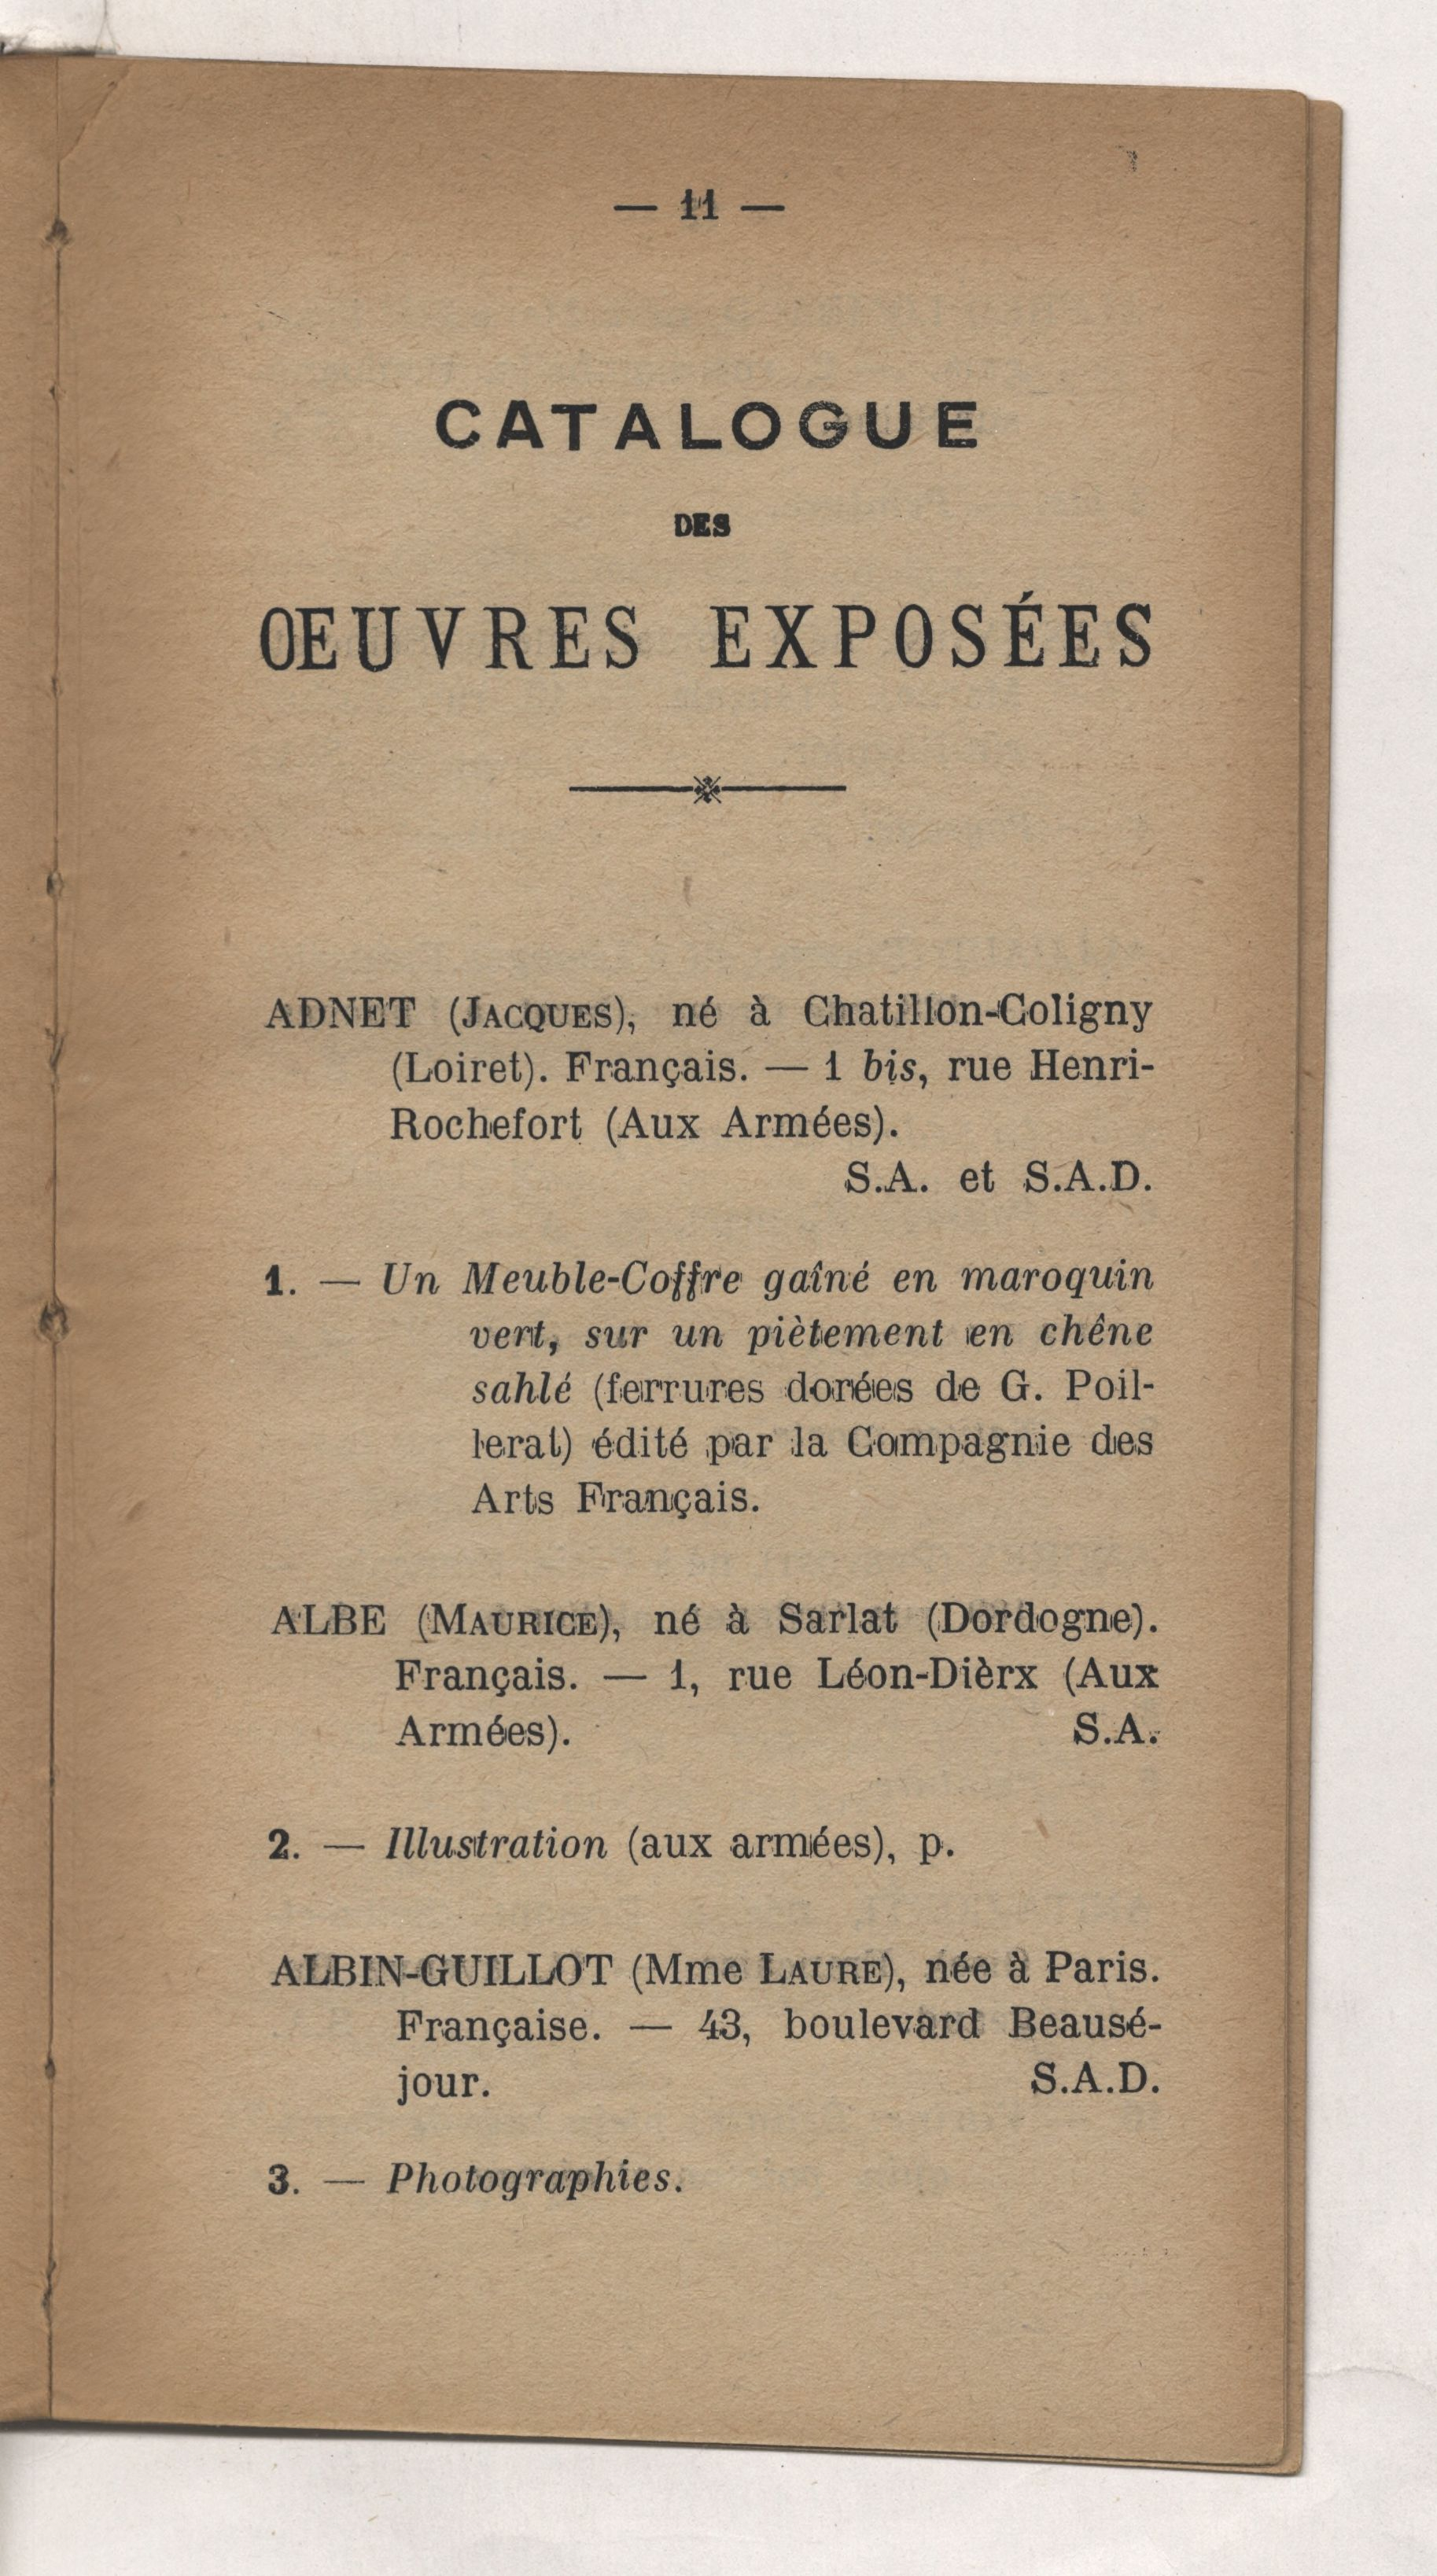
\includegraphics[scale=0.7]{image_1}		
	\caption{\texttt{input} : exemple de page de catalogue (Salon d'automne 1940)}
	\label{page11}
\end{figure}

\begin{figure}[ht]
	\centering
	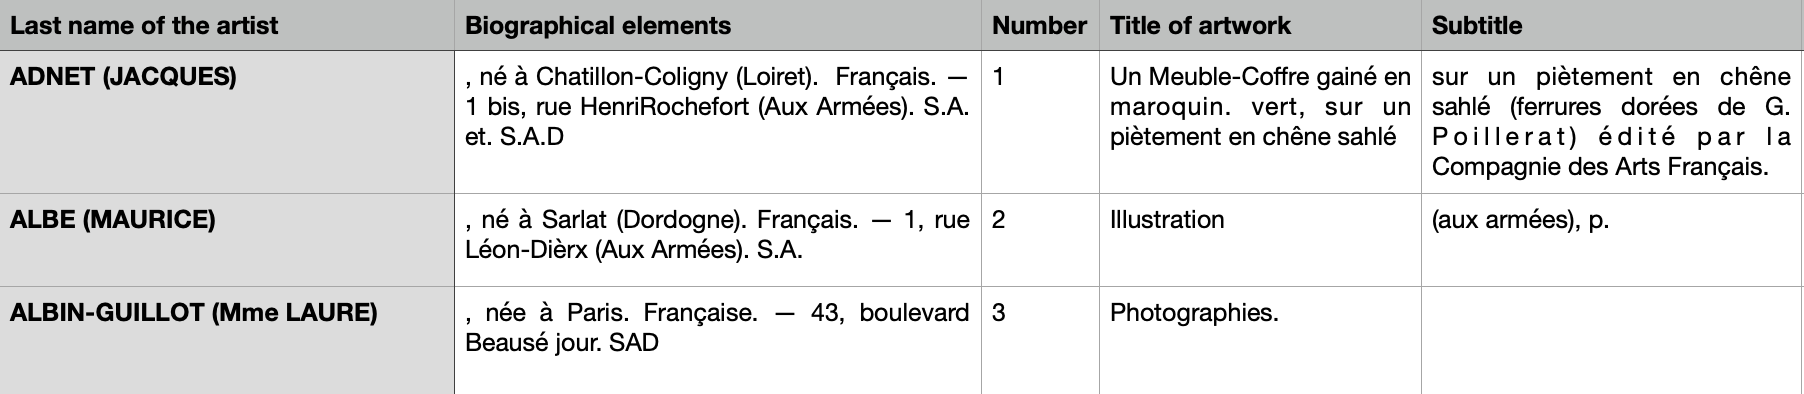
\includegraphics[scale=0.5]{tableau_automne}		
	\caption{\texttt{output} : tableur contenant les informations de la page de catalogue}
	\label{tableur11}
\end{figure}

Comme cela est décrit dans les parties précédentes, les interactions humaines avec les logiciels sont conçues dans (ou adaptées à) un but pédagogique. Les interventions, vérifications et corrections virtuellement nécessaires sont normalement connues et les utilisateurs sont en conséquence censés en êtres avertis. Si la prise en main de ce pipeline nécessite d'un apprentissage technique (qui en est l'objetcif primordial), les résultats acquièrent une performance exponentielle dès lors qu'il s'agit de traiter des corpus conséquents. Rappelons qu'avant la mise en place des stages Artl@s/TNAH, la saisie des tableurs était entièrement manuelle et impliquait donc un investissement temporel extrêmement poussé. Au stade actuel, c'est la saisie manuelle des régions (liée à l'inexistence de modèles de segmentation satisfaisants), puis la correction manuelle des transcriptions automatiques (qui sont de manière générale très efficaces) qui vont demander le plus de temps. 
Un dernier enjeu, plus explicite lors du stage de Juliette Janès, reste une dimension constitutrice de notre travail : les technologies numériques utilisées sont des outils \textit{Open Source} fondamentaux dans le domaine des humanités numérique. L'objectif de rendre le pipeline conforme aux préconisations pour la science ouverte\footcite{unesco_vers_2019} est repoussé à un nouvel horizon dans le mesure où il s'agit maintenant de former et/ou d'accompagner des chercheurs dans le développement d'une culture numérique solide, susceptible de contribuer à normaliser des échelons supérieurs d'autonomie technique dans l'univers des sciences humaines.

Le pipeline semi-automatique extractionCatalogs (océrisation avec eSCriptorium + extraction avec le script extractionCatalogs), accompagné par un guide d'utilisation à vocation pédagogique (Jupyter notebook), a donc un intêret scientifique (produire des instruments pour la recherche), technique (produire efficacement ces instruments) et pédagogique (présenter des technologies numériques fondamentales dans le domaine des humanités numériques). Elle comporte les deux grandes étapes suivantes, dont la description sera approfondie dans les chapitres qui suivent :


\begin{enumerate}
	\item L'utilisation d'eScriptorium, un logiciel de recconnaissance de caractères (OCR) pour transcrire automatiquement des pages (images) numérisées de catalogue. eScriptorium est une interface qui permet de visualiser toute la chaîne de traitement OCR des images. Ce traitement est en réalité effectué par Kraken, un logicel qui permet d'entraîner et d'appliquer des modèles de reconnaissance de caractères ainsi que des modèles de segmentation de page
	\begin{itemize}
		\item \texttt{input} : des images numériques de catalogues du XIXe et XXe siècle issues d'un manifeste \texttt{iiif} ou en format \texttt{.jpg}, \texttt{.png}, etc.)
		\item l'utilisateur/utilisatrice applique un modèle efficace pour que la machine face une transcription automatique des pages
		\item l'utilisateur/utilisatrice doit faire des corrections manuelles de la transcription automatique, sur l'interface même
		\item l'utilisateur/utilisatrice doit aussi segmenter manuellement ces pages, cet à dire saisir et nommer ses régions sémantiques (il/elle doit signaler où se trouvent les entrées de catalogue dans une image). Dans le projet Artl@s, le choix du nom des régions est conforme a l'ontologie Segmonto (un standard efficace de nommage des zones dans une page)

		\item \texttt{output} : l'utilisateur/utilisatrice obtiendra en sortie des fichiers XML ALTO4, un type de document adapté à l'encodage des catalogues, puisqu'il tient compte de la localisation spatiale des éléments de la page. Chaque image numérique sera transcrite dans un fichier ALTO ; nous obtiendrons donc un fichier Alto pour chaque page de catalogue
	\end{itemize}
	
	\item L'utilisation du programme extractionCatalogs, qui traite les données produites lors de l'étape antérieure, pour produire les fichiers souhaités (restructurations ALTO, encodage en XML-TEI et tableurs CSV)
	\begin{itemize}
		\item \texttt{input} : des fichiers XML ALTO4 produits par l'interface eScriptorium
		\item lancement du script avec la commande suivante :
		\begin{normalsize}
			\begin{minted}{bash}
!python3 run.py   chemin_input   chemin_output   nom_du_catalogue
			\end{minted}
		\end{normalsize}
		\item le script, écrit dans le langage de programmation Python 3, comporte de multiples fonctions qui traitent automatiquement les fichiers en entrée. Pour chaque fichier ALTO (qui comporte l'encodage d'une page individuelle de catalogue), il analyse le document ligne par ligne pour reconstituer le catalogue, entrée par entrée. De manière générale, une entrée est constituée des éléments suivants : nom de l'exposant, informations biographiques/complémentaires, liste des oeuvres présentées (avec des éventuelles informations complémentaires)
		\item \texttt{output} : fichier XML-TEI (encodage structuré) : un seul fichier contenant tout le catalogue et signalant sa structure à partir de balises. Ces balises (par exemple \texttt{<name>MONET (Claude)</name>}) signalent les entrées, les exposants, les oeuvres, les informations complémentaires, etc.		\item \texttt{output} : tableurs CSV : les mêmes informations sont présentées sous forme de tableaux : un tableau adapté à la base de données BasArt du projet Artl@s, et qui sera normalement utilisée pour l'alimenter, ainsi qu'une version simplifiée. Cette dernière est conçue pour être comprise aisément par un être humain
		\item \texttt{output} : fichier \texttt{.txt} indiquant des problèmes d'extraction, pour que l'utilisateur/utilisatrice puisse faire des corrections manuelles. Ce document résulte d'un travail approfondi de localisation et de gestion des erreurs attendues (non-conformité des documents en \texttt{input}, erreurs de transcription et de segmentation, etc.) 
	\end{itemize}
\end{enumerate}



	\chapter{Installation : répositoire et Jupyter notebook}
	\label{installation}
	
Ce chapitre décrit les installations nécessaires pour pouvoir utiliser le script python extractionCatalogs avec le guide/interface Jupyter Notebook. Outre le répositoire avec le programme, il est nécessaire de lancer (ou d'installer et de lancer) Jupyter Notebook ainsi qu'un paquet d'extensions appelé \texttt{jupyter\_contrib\_nbextensions}. Celui-ci facilite une expérience plus "User Friendly" en permettant de visualiser une table des matières avec une structure collapsable. Le guide prévoir qu'un néophyte soit capable de faire ces installations rapidement. 

\section{Installer le répositoire : altérnatives}

Il est possible de télécharger uniquement le script python, et de l'utiliser en lançant la commande du programme sur un terminal. Cet usage n'est pas recommandé pour des utilisateurs sans expérience, mais il permet de travailler sans la médiation du Notebook et fonctionne de manière autonome. Comme l'indique le fichier \texttt{README.md} sur le répositoire Github du projet, il faut utiliser le "Version Control System" Git, qu'il est possible de télécharger pour Mac, Windows et Linux en suivant les indications du site officiel.\footcite{Git}


Git fournit les commandes qui permettront de télécharger depuis Github\footcite{Github} le répertoire (projet sous forme d'arborescence de dossiers) du programme extractionCatalogs\footcite{ExtractionCatalogs}. Il faut ouvrir un terminal et lancer les commandes suivantes :
	
\begin{enumerate}
	\item Pour la première installation :
	\begin{itemize}
		\item cloner le répositoire : 
		\mint{bash}|git clone https://github.com/Juliettejns/extractionCatalogs|
		\item créer un environnement virtuel : \texttt{virtualenv -p python3 env}
		\item activer l'environnement virtuel : \texttt{env/bin/activate}
		\item installer les \textit{packages} python nécessaires : \texttt{pip install -r requirements.txt}
	\end{itemize}
	\item Pour lancer l'application après la première installation :
	\begin{itemize}
		\item Se déplacer sur le dossier du répertoire installé localement
		\item activer l'environnement virtuel : \texttt{env/bin/activate}
	\end{itemize}
\end{enumerate}

Cependant, dans le cas d'usage normal à travers du guide Jupyter Notebook, ces installations via le terminal ne sont pas nécessaires. Le guide permet en effet de lancer les commandes en son sein même, ce qui facilite la prise en main pour les étudiants. 


\section{Installer et configurer le guide : Jupyter notebook et nbextensions}


Béatrice Joyeux-Prunel et Simon Gabay travaillent avec leurs étudiants du certificat en humanités numériques de l'Université de Genève à travers de Google Colab, un environnement en ligne qui permet d'exécuter du code. Celui-ci est utilisé pour conserver le répositoire et les installations python, qui peuvent dès lors être lancées sur un navigateur web. Il suffit donc que les étudiants aient le lien vers le notebook pour commencer à exécuter les instructions qui suivent. Autrement, il suffirait qu'ils aient en local les fichiers \texttt{Guide – extraction de catalogues.ipynb} et \texttt{requirements.txt}, qu'ils ouvrent un terminal et qu'ils tapent les commandes suivantes : 
	\begin{itemize}
		\item aller vers le dossier contenant les fichiers
		\item créer un environnement virtuel : \texttt{virtualenv -p python3 env}
		\item activer l'environnement virtuel : \texttt{env/bin/activate}
		\item lancer Jupyter notebook (un navaigateur s'ouvrira automatiquement) : 
		\mint{bash}|Jupyter Notebook|
		\item continuer en suivant les indications du Notebook
	\end{itemize}

Ces manipulations à travers du terminal ne sont pas nécessaires puisque les étudiants peuvent normalement accéder directement au Notebook avec un lien.\\

\subsection{Jupyter Notebook}

Jupyter Notebook\footcite{JupyterNotebook} est un logiciel qui permet d'afficher sur un navigateur des fichiers \texttt{.ipynb}, qui présentent des morceaux de code commentés. Cet outil fondamental dans des cadres universitaires (recherche et enseignement) permet donc d'expliquer convenablement le fonctionnement de scripts. Sur un notebook Jupyter, il existe deux types de cellule : soit pour afficher et exécuter du code, soit pour écrire en MarkDown\footcite{MarkdownguideOrg} (un langage à balise extrêmement simple). Ces dernières sont utilisées pour accompagner le code de commentaires et d'images.

La prise en main de Jupyter Notebook est rapide ; le guide commence en expliquant aux étudiants les manipulations basiques qui leur permettront de lancer le code dans les cellules :
\begin{itemize}
	\item pour exécuter une cellule de code : taper SHIFT/ENTER, ou bien COMMAND/ENTER sur mac, ou bien le bouton \texttt{Run} sur le menu de la page
	\item une cellule de code qui commence avec un point d'exclamation (\texttt{!}) n'exécute pas du code, mais une commande sur le terminal. 
\end{itemize} 

Il est donc possible d'installer tout le programme et ses \textit{packages} en exécutant une seule cellule. Il suffit pour cela d'avoir le fichier \texttt{Guide – extraction de catalogues.ipynb} en local, de l'ouvrir avec un terminal (commande \texttt{Jupyter Notebook}) et d'exécuter une cellule contenant les commandes suivantes : 

\begin{normalsize}
	\begin{minted}{bash}
		!git clone https://github.com/Juliettejns/extractionCatalogs
		!virtualenv -p python3 env
		!pip install -r requirements.txt
	\end{minted}
\end{normalsize}

\subsection{nbextension : extensions pour Jupyter Notebook}

Après les installations fondamentales, le guide invite l'utilisateur à installer le paquet \texttt{nbextension}\footcite{JupyterNotebookExtensions}. À nouveau, cela se fait de manière extrêmement simple à travers d'une cellule du Notebook, et permet que celui-ci devienne une interface aisément navigable avec une table des matières interactive et des sections (chapitres et sous-chapitres sur plusieurs niveaux) "collapsables". Les installations se font en exécutant une seule cellule contenant le code suivant : 
\begin{normalsize}
	\begin{minted}{bash}
!jupyter contrib nbextension install --user
!pip install jupyter_nbextensions_configurator
!jupyter nbextensions_configurator enable --user	
	\end{minted}
\end{normalsize}

Ce paquet intègre et active un nouvel onglet sur la page, qui permet d'activer et de désactiver plusieurs add-on (fonctionnalités ajoutées). L'utilisateur doit faire les manipulations suivantes (voir figure \ref{confignextensions}):
\begin{enumerate}
	\item cliquez sur le logo "Jupyter" en haut à gauche de la page
	\item cliquez sur l'onglet "nbextensions"
	\item activez les extensions "collapsable Headings" et "Table of contents (2)"
\end{enumerate}

\begin{figure}[ht]
	\centering
	\includegraphics[scale=0.4]{jupyter_extensions_1.png}		
	\caption{Activation de la table des matières et des sections collapsables}
	\label{confignextensions}
\end{figure}

En cliquant sur ces extensions, l'utilisateur accède à leurs menus, dans lesquels il doit cocher les cases suivantes pour activer des options :

Dans le menu de l'add-on Collapsable Headings :

\begin{itemize}
	\item \texttt{"Collapse/uncollapse notebook sections when the ToC2 nbextension is used to collapse/uncollapse sections in the table of contents. For the inverse behaviour, see ToC2's configuration"}
\end{itemize}

Dans le menu de l'add-on Table of Content (2) :
\begin{itemize}
	\item \texttt{"Skip h1 headings from numbering, so that they can serve as a notebook title. See the README for details, caveats and alternatives"}
	\item \texttt{"Collapse/uncollapse ToC sections when the collapsible\_headings nbextension is used to collapse/uncollapse sections in the notebook. For the inverse behaviour, see collapsible\_headings' configuration"}
\end{itemize}


L'utilisateur peut désormais rafraichir la page pour accéder à une interface beaucoup plus simple à utiliser (voir figure \ref{interfacenb}) : au lieu d'avoir un long document, il est maintenant possible d'observer les sections et de déplier uniquement celles qu'il a besoin de consulter. Dans le cadre de son travail, l'utilisateur peut ainsi mettre de côté les étapes qu'il a déjà pris en main. 

\begin{figure}[ht]
	\centering
	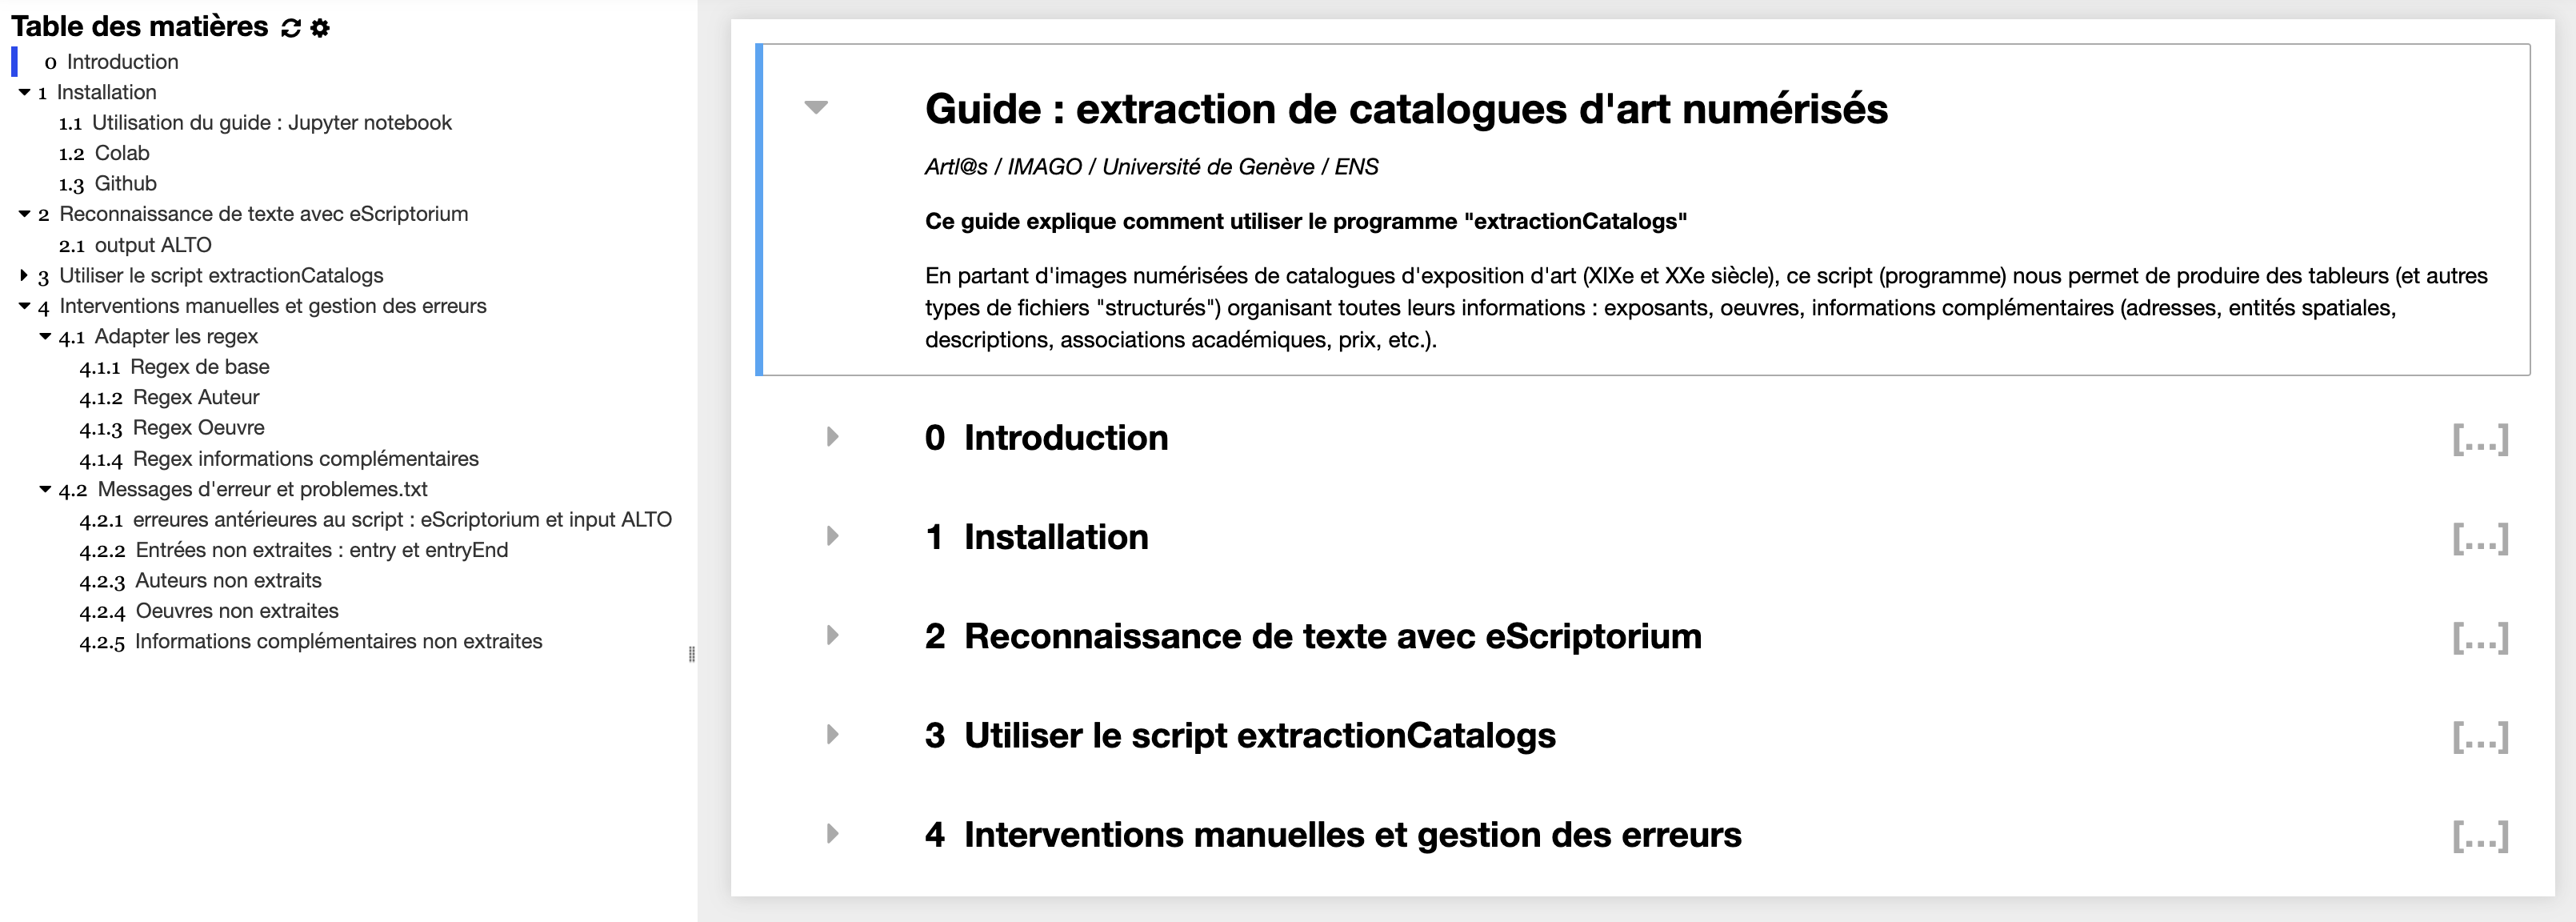
\includegraphics[scale=0.2]{menu_guide.png}		
	\caption{Table des matières du notebook}
	\label{interfacenb}
\end{figure}

Normalement, c'est après cette installation que l'étudiant lancera une cellule qui installe les \texttt{packages} python du script extractionCatalogs à proprement parler. Les mentions antérieurs de commandes sur le terminal (directement ou sur une cellule du notebook avec le signe "\texttt{!}") relatives au répositoire ne font pas partie du guide et présentent des manières alternatives de faire les installations. En effet, il suffit pour l'étudiant d'exécuter la cellule suivante pour avoir une installation complète et fonctionnelle (si cela est fait à partir du lien Google Colab, méthode choisie par les responsables du certificat en humanités numériques) : 

\begin{normalsize}
	\begin{minted}{bash}
!pip install -r requirements.txt
	\end{minted}
\end{normalsize}

Cette commande installe les paquets(\textit{packages}) python nécessaires pour que le script fonctionne correctement. Les \textit{packages} sont des sous-ensembles du langage de programmation python qui ne sont pas intégrés à la version de base, et qui sont conçus pour être appelés ou installés à la demande des utilisateurs pour des besoins spécifiques.

La céllule affiche alors les messages du terminal, qui donnent des informations sur le processus qui vient d'avoir lieu. Le script va produire des messages qui peuvent être très longs en fonction du catalogue, puisqu'ils signalent toutes les entrées extraites. De ce fait, il est important de rappeler qu'il est possible d'augmenter ou de diminuer la taille d'une cellule en cliquant ou en double-cliquant l'espace en blanc à à gauche de celle-ci:

\begin{figure}[ht]
	\centering
	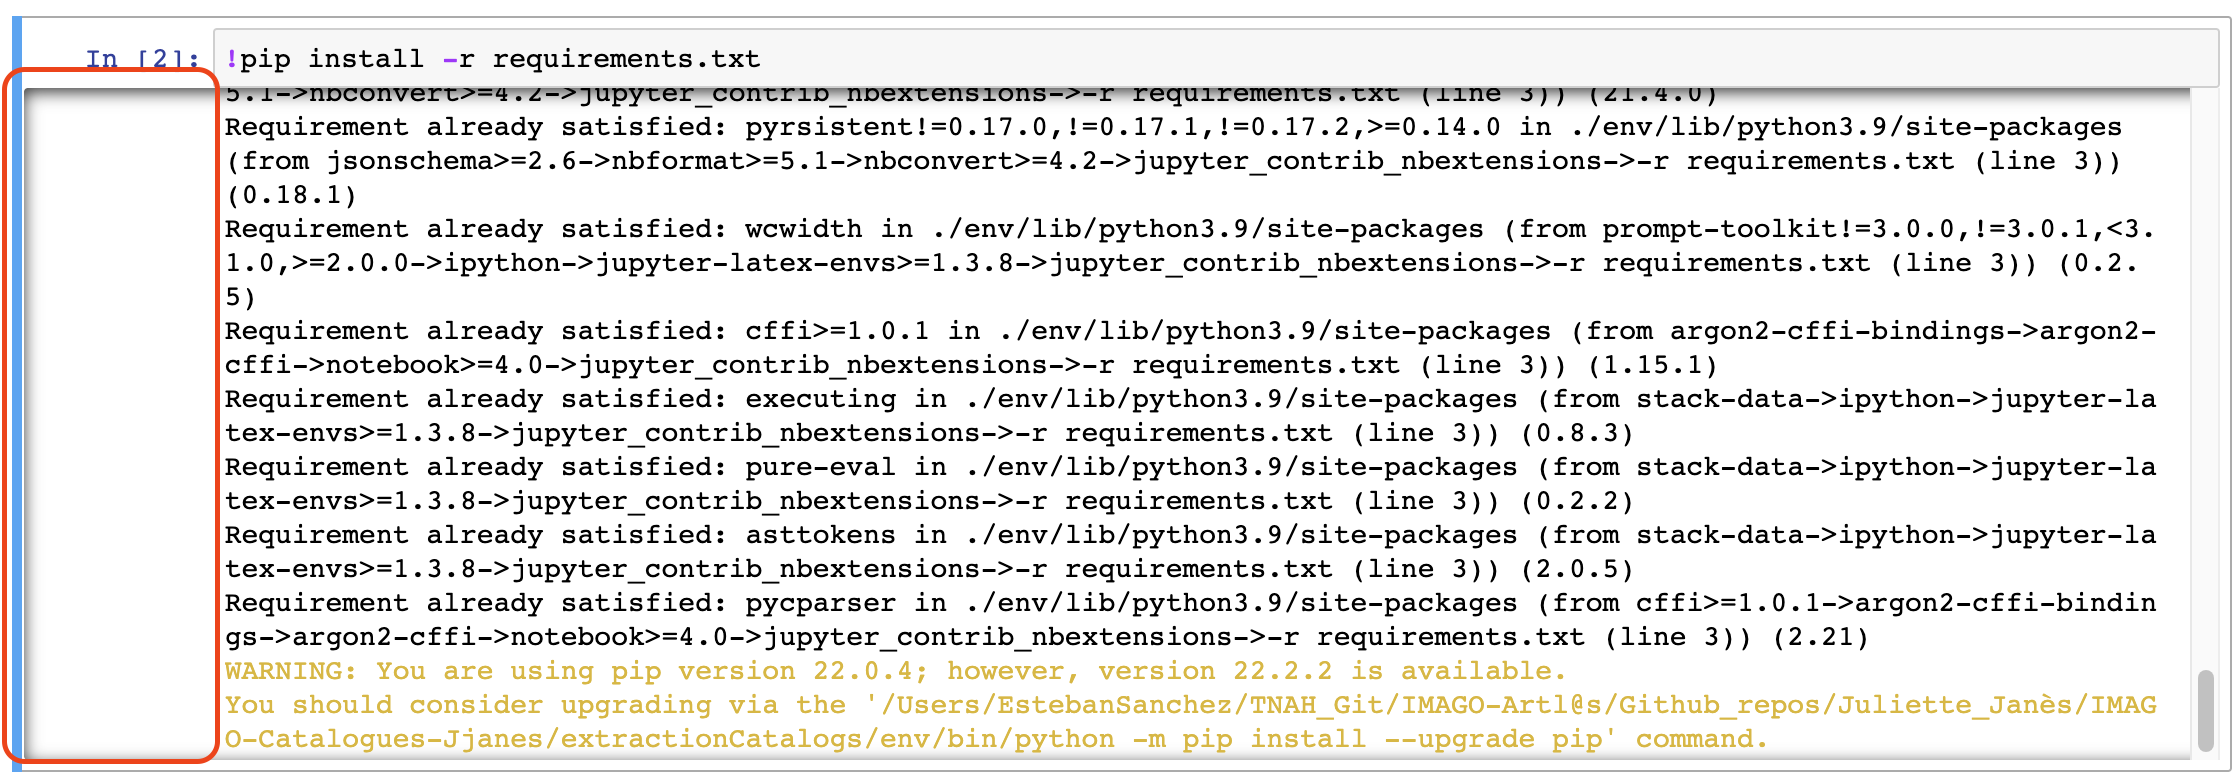
\includegraphics[scale=0.3]{cellule_diminuer.png}		
	\caption{Diminuer une cellule sur le notebook}
\end{figure}

À présent, le processus d'installation est terminé. L'utilisateur a lancé ses premières commandes sans avoir à utiliser un terminal, et a effectué l'installation de \texttt{packages} python sans difficulté. Après cet apprentissage rudimentaire sur l'installation et l'utilisation d'un notebook, il possède une interface qui l'accompagnera à travers de tout le pipeline.




	\chapter{Reconnaissance de caractères : interface eScriptorium}
	

	

L'utilisation de l'interface eScriptorium constitue le début du pipeline à proprement parler. Ce logiciel HTR et OCR fonctionne comme une interface graphique faisant tourner kraken, un programme normalement accessible uniquement à travers d'un terminal \texttt{bash}. Pour plus d'informations sur ces technologies, veuillez consultez le chapitre 1.3 du présent mémoire.

eScriptorium permet l'utilisation de kraken par des personnes sans compétences informatiques particulières, d'une manière en principe intuitive et confortable. Il est toutefois important de détailler les consignes à suivre, puisque eScriptorium peut poser quelques contraintes techniques et la démarche à suivre aura un impact dans les fichiers ALTO qu'il produit en \texttt{output}. De plus, la prise en main peut paraître évidente pour des usagers habitués ou pour des personnes avec une culture numérique avancée, mais les retours d'étudiants rendent manifeste que l'apprentissage et la compréhension de l'interface ne sont pas immédiats. Pour ces raisons, une description technique et mécanique de l'utilisation préconisée s'avère nécessaire.


\section{OCR avec eScriptorium et Kraken}

eScriptorium permet de transcrire et de segmenter des pages avec du texte, automatiquement aussi bien que manuellement. Cela permet une dynamique fluide entre la machine et l'être humain, puisque la possibilité de faire des interventions et des corrections manuelles est au centre de l'interface. Dans le cas des catalogues d'exposition d'art du XIXe siècle, le modèle de reconnaissance de caractères implémenté sur eScriptorium est extrêmement efficace. En effet, le modèle \texttt{HTRcatalogs Artlas} a été développé pour le projet Artl@s même. Le résultat de la transcription nécessite tout de même de vérifications et de corrections manuelles plus ou moins importantes selon le catalogue ; une extraction correcte avec le script python dépend en très grande partie de l'exactitude de la transcription (en particulier les chiffres ou autres caractères permettant de signaler des oeuvres, des exposants, ou de séparer les éléments de la page). 

La deuxième étape, fondamentale, consiste dans la segmentation des pages, c'est à dire dans la signalisation de ses régions sémantiques (notamment les entrées de catalogue). Les informations de segmentation sont utilisées par le script python pour chercher et reconstituer les entrées, ainsi que pour mettre de côté des informations non pertinentes. Les catalogues d'exposition sont des documents structurés avec des configurations particulières qui permettent de comprendre visuellement la signification des régions contenant du texte, de par leur disposition dans la page ou de par les caractéristiques typographiques du texte. Cette information visuelle, immédiate ou très rapidement appréhendable par l'œil humain, n'est pas discernable par la machine. Kraken permet d'entrainer des modèles de segmentation automatique, mais aucun n'est satisfaisant dans le cadre du corpus traité. En attente de modèles performants, l'utilisateur devra faire la segmentation sur eScriptorium manuellement, page par page. La production de fichiers ALTO avec des régions saisies manuellement pourrait contribuer à terme à entrainer des modèles satisfaisants pour ce projet.

Dans le cadre de cette étape, nous fournirons en \texttt{input} des images numériques de catalogues du XIXe et XXe siècle. L'interface accepte les principaux types de fichier image, comme \texttt{.jpg}, \texttt{.png} ou  \texttt{.pdf}. Il est cependant vivement conseillé d'utiliser un manifeste iiif, un standard de partage d'images qui sera présenté dans les pages suivantes.
En \texttt{output}, eScriptorium fournira un fichier XML-ALTO4 pour chaque image traitée ; ces fichiers seront utilisées lors de la deuxième étape du pipeline (script python extractionCatalogs). ALTO est un standard XML choisi dans le cadre du projet Artl@s car il permet d'encoder efficacement la répartition spatiale du texte dans la page. Le script a été conçu pour traiter uniquement ce type de fichier. 

Le notebook propose aux utilisateurs de suivre le guide en traitant le catalogue de leur choix. Il expose les étapes à travers d'un exemple représentatif des cas usuels, un catalogue d'une exposition d'art aillant eu lieu à Nancy en 1843 \footcite{societelorrainedesamisdesartsCataloguePeinturesMiniatures1843}. Il s'agit d'un catalogue court de 24 pages, dont uniquement 13 avec des entrées à proprement parler. Il sera utilisé aussi comme exemple dans les pages suivantes pour exposer le fonctionnement du pipeline du début à la fin.

Dans le cadre de ce pipeline, nous pouvons distinguer trois étapes dans l'utilisation d'eScriptorium : la mise en place du projet (gestion des paramètres préliminaires, des images et des noms des zones), la transcription automatique du texte contenu dans les images, et la segmentation manuelles des régions contenues dans les images.

\section{Mettre en place un projet sur eScriptorium}

En 2022, le stage Artl@s a mis de côté le travail et les réflexions sur la reconnaissance de caractères. En principe, cela dérive d'une division du travail sur les missions de plusieurs stagiaires. Il s'agissait de produire un script d'extraction performant et directement exploitable dans un cadre pédagogique, tandis que le stage de Paul Kervegan s'est penché sur l'entraînement de modèles de segmentation sur kraken avec Simon Gabay. Le présent travail n'aborde donc la question que dans le cadre de l'utilisation de l'interface eScriptorium, et plus spécifiquement des outils et modèles qu'elle met à disposition. 

eScriptorium permet de gérer intuitivement toutes les étapes de production de transcriptions, que ce soit à travers d'outils automatiques ou de saisies manuelles. Le projet Artl@s s'ajute à certains standards de nommage et de saisie des régions, et le script extractionCatalogs nécessite que certains éléments en \texttt{input} soient ajustés à son traitement des fichiers ALTO. Pour cette raison, il est fondamental d'expliquer aux utilisateurs comment utiliser eScriptorium de manière extrêmement précise : on s'est rendu compte  pendant la mission que l'ordre et les pratiques de saisies ont un impact sur la structure des fichiers en \texttt{output}. eScriptorieum est une interface en développement constant, et ses fonctionnalités ne peuvent être pleinement adaptées aux cahiers des charges du projet Artl@s. C'est sur la question des segmentations manuelles qu'il faudra être le plus vigilant, mais le script extractionCatalogs permet maintenant de restructurer et de corriger selon nos besoins les fichiers produits par eScriptorium. 

On va donc présenter ici, étape par étape, les bonnes pratiques d'utilisation d'eScriptorium et leurs enjeux dans le cadre du projet Artl@s. Les étudiants du certificat en humanités numériques de l'Unige ont accès à FonDue\footcite{FoNDUE} (FOrmes numérisées et détection unifiée des ecritures), une versions d'eScriptorium sur les serveurs locaux de l'université. Il est également possible de suivre les instructions à partir de tout autre installation de l'interface.


\subsection{Créer un projet}

Voici les étapes à suivre pour créer un projet eScriptorium :

\begin{itemize}
	
\item Premièrement, l'utilisateur est invité à créer un projet nouveau en allant sur l'onglet "my projects", et en cliquant sur "Create New Project" 
\begin{figure}[ht]
	\centering
	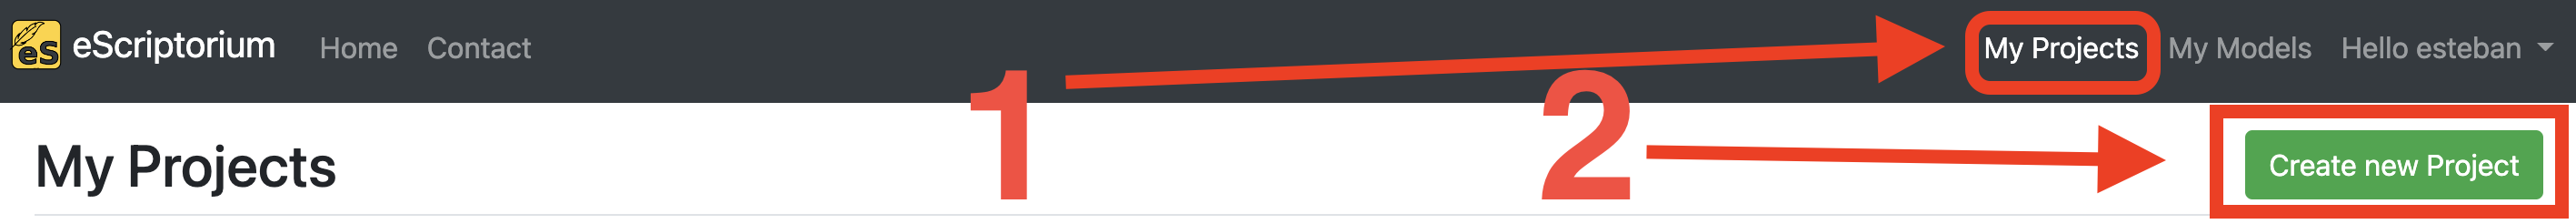
\includegraphics[scale=0.3]{projet_eScriptorium.png}		
	\caption{eScriptorium : créer un projet}
\end{figure}

\item Il devra choisir un nom pour le catalogue, puis cliquer sur "Create" (figure \ref{create1})
\begin{figure}[ht]
	\centering
	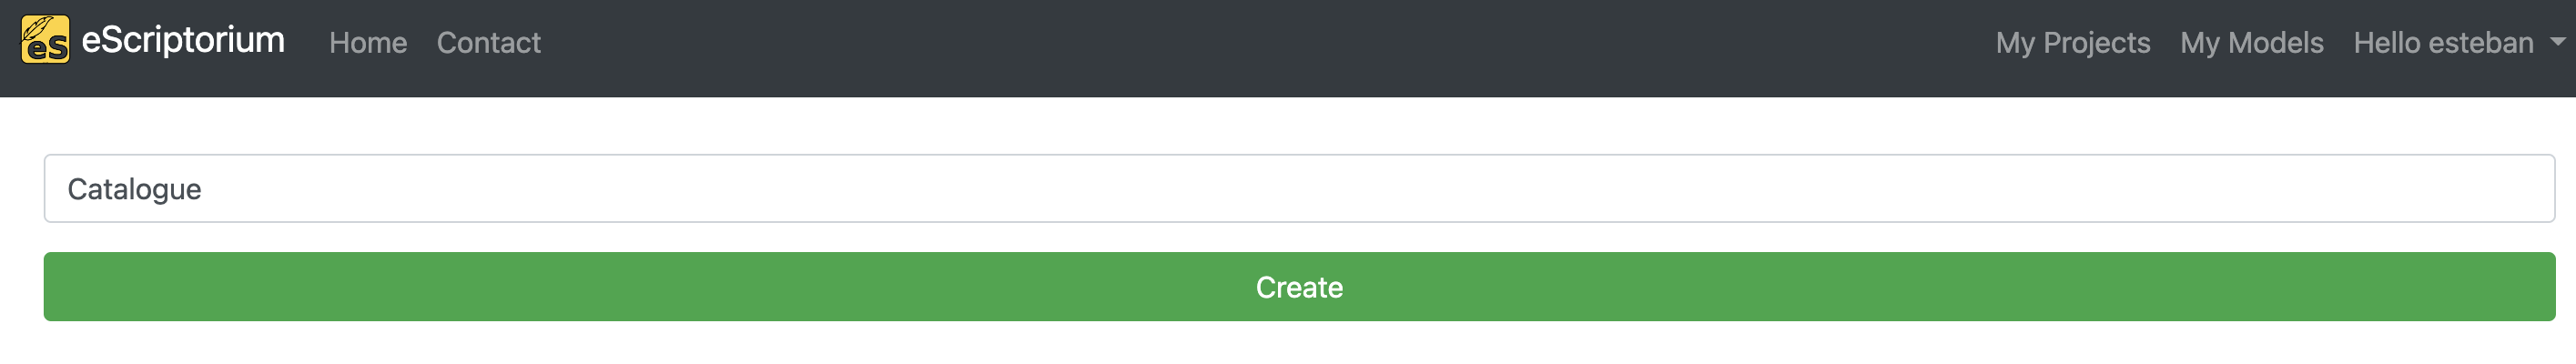
\includegraphics[scale=0.3]{create_eScriptorium.png}		
	\caption{eScriptorium : créer un projet (2)}
	\label{create1}
\end{figure}

\item Il faut ensuite cliquer sur le projet pour accéder à sa page (figure \ref{create3})
\begin{figure}[ht]
	\centering
	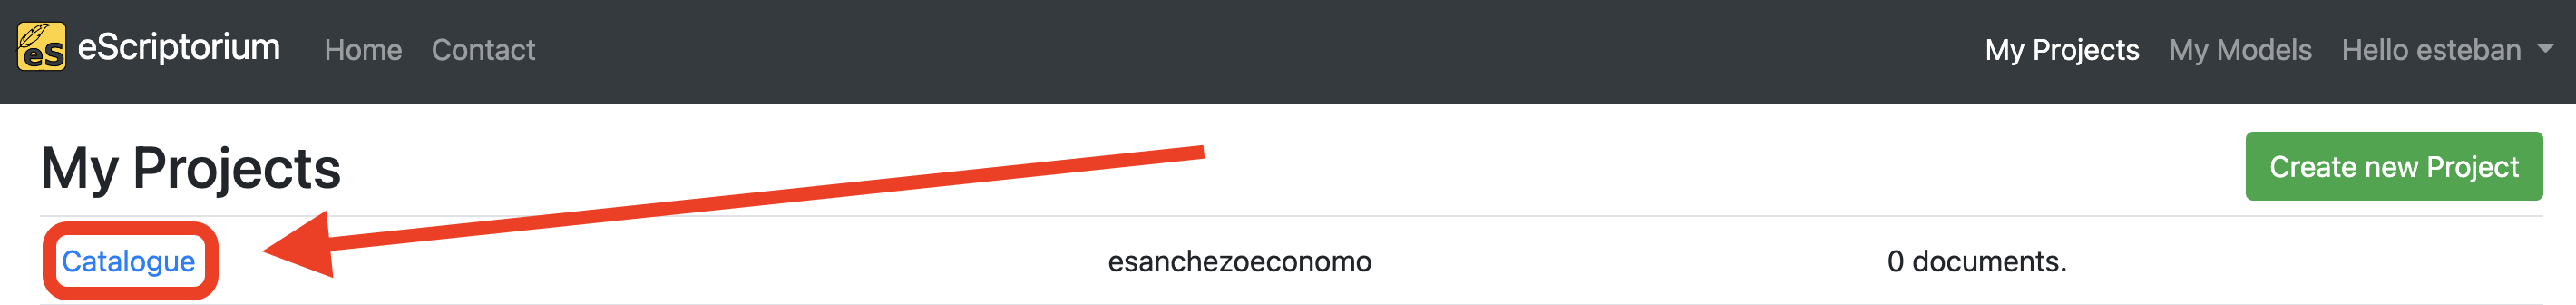
\includegraphics[scale=0.3]{document_eScriptorium.png}		
	\caption{eScriptorium : créer un projet (3)}
	\label{create3}
\end{figure}

\item Puis cliquer sur "Create new Document" (figure \ref{create4})
\begin{figure}[ht]
	\centering
	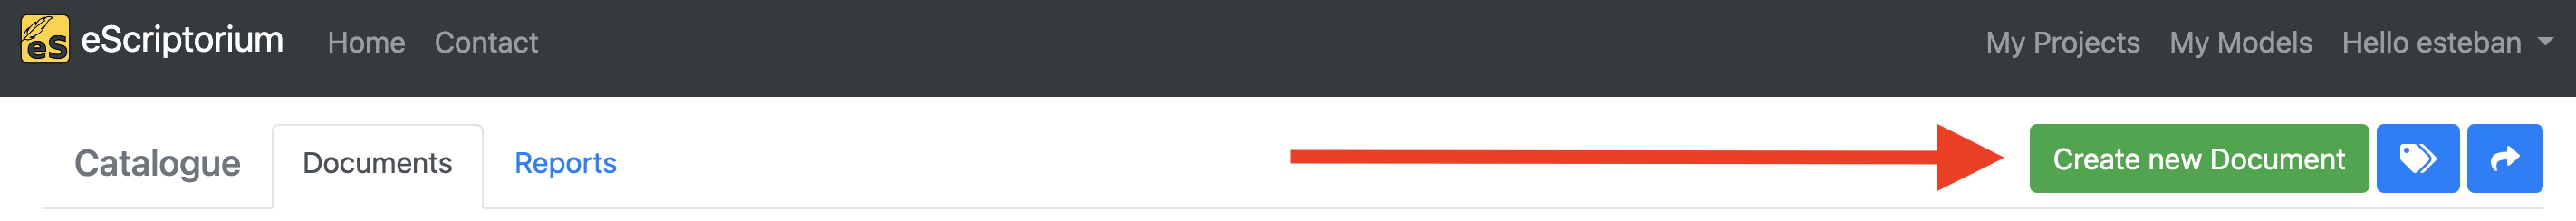
\includegraphics[scale=0.3]{new_document_eScriptorium.png}		
	\caption{eScriptorium : créer un projet (4)}
	\label{create4}
\end{figure}

\item Il faudra ensuite [1] Choisir un nom pour le document et [2] cliquer sur "Create" (figure \ref{create})
\begin{figure}[ht]
	\centering
	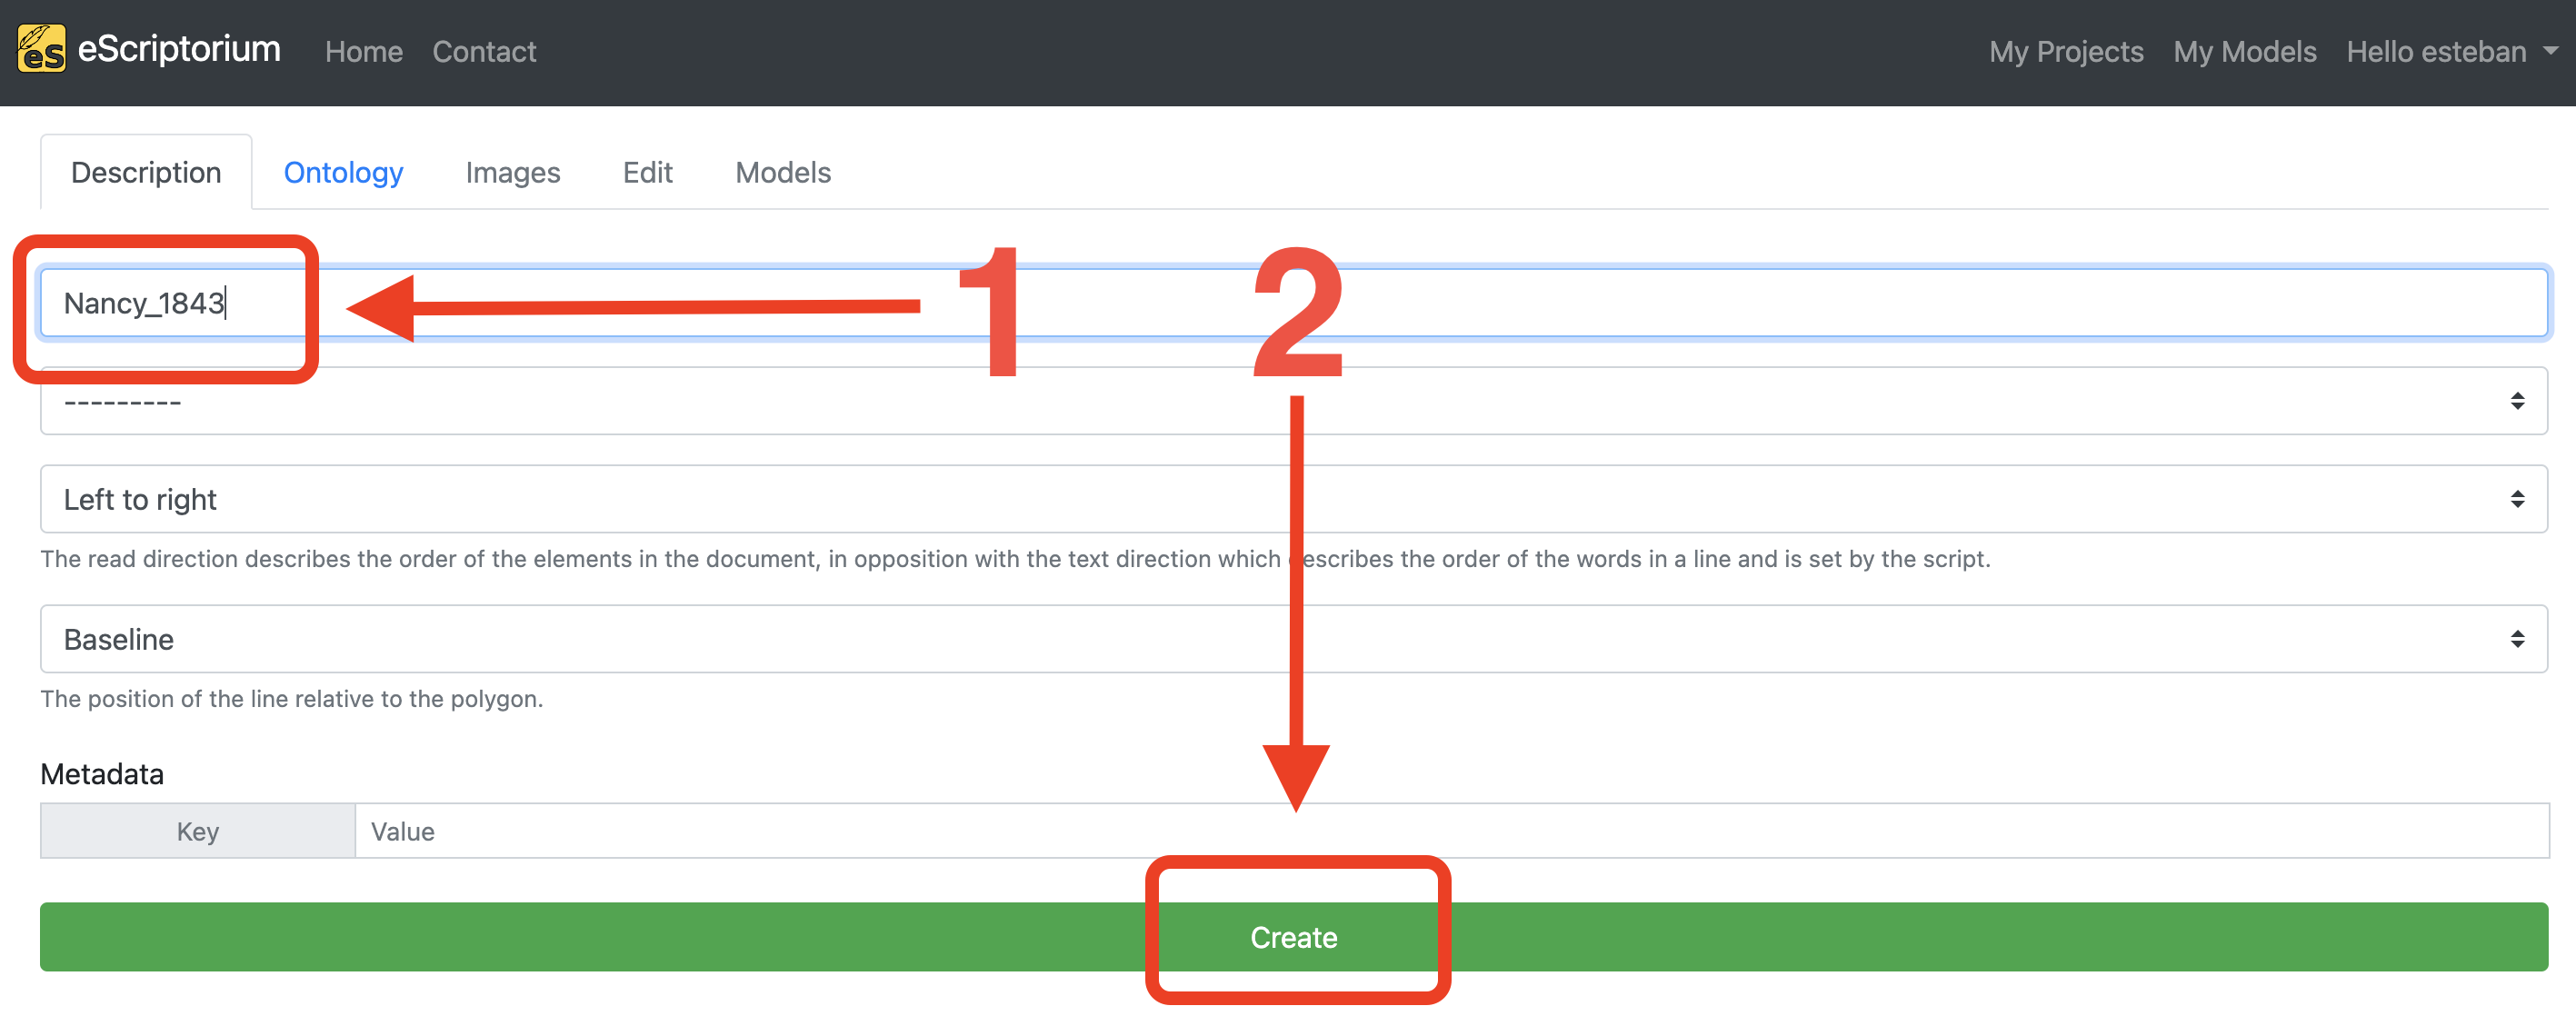
\includegraphics[scale=0.2]{create_doc_eScriptorium.png}		
	\caption{eScriptorium : créer un projet (5)}
	\label{create}
\end{figure}
\end{itemize}

Ces étapes préliminaires permettent de créer un projet et un document dans ce projet. Les étapes suivantes consistent à établir les noms des zones (cela permettra après de faire la segmentation) puis à ajouter des images. 


	\subsection{L'Ontologie Segmonto}

Pour signaler les zones qui existent dans chaque page du catalogue, le projet Artl@s préconise d'utiliser l'ontologie Segmonto\footcite{noauthor_segmonto_nodate}. À ce stade, le script a été adaptée à cette ontologie, et en a donc besoin pour pouvoir fonctionner. 

Segmonto est un standard de nommage des zones, un vocabulaire contrôlé pour décrire la page manuscrite et imprimée
\footcite{gabayFourthParadigmDigital2022,gabayFourthParadigmDigital2022}
. Son utilisation implique deux avantages immédiats. Premièrement, l'ontologie est issue de discussions et de réflexions menées par des spécialistes en humanités numériques et en philologie, et propose un protocole cohérent et scientifiquement robuste pour nommer les zones d'une page. Deuxièmement, ce standard extrêmement récent est l'une des premières réponses à un intérêt croissant envers le développement de modèles de segmentation automatiques satisfaisants. Il se généralise rapidement (par exemple, il sera prochainement intégré à l'interface eScriptorium, de manière à que l'utilisateur n'aie plus à saisir les noms manuellement), ce qui renforce la compatibilité du projet Artl@s avec d'autres. Dans ce cadre, le script extractionCatalogs fournit des fonctions qui pourraient elles mêmes s'avérer utiles pour adapter l'\texttt{output} d'eScriptorium à d'autres traitements focalisés sur les régions saisies.

Segmonto propose de nombreuses zones de page décrites, et le standard évolue de manière à rajouter des niveaux de précisions adaptés aux besoins de chaque projet. Un ajout récent est la possibilité d'annexer à un type de région standard, après deux points ":", des sous-types et/ou des chiffres mieux adaptés au contexte du projet (par exemple \texttt{MainZone:column\#1.}).\\

La liste suivante montre les noms de zone qui ont été sélectionnés dans l'ontologie pour décrire les régions d'une page de catalogue : 

\begin{itemize}
	\item \texttt{MainZone} : cette zone fait référence à la totalité de l'espace sémantique de la page. Dans les catalogues Artl@s, elle doit contenir la totalité des entrées et du texte, et exclure des éléments qui ne font pas partie du contenu sémantique de la page,  tels que le numéro de page ou des titres courants
	\item \texttt{CustomZone:entry} : \texttt{CustomZone} est un type de zone qui permet à l'utilisateur d'ajouter un nom de son choix ; il indique ainsi un type de zone créé par l'utilisateur. Il était nécessaire de créer une zone adaptée aux entrées de catalogues. une entrée (CustomZone:entry) est composée d'un exposant et des œuvres qu'il expose, avec toutes les informations complémentaires concernées
	\item \texttt{CustomZone:entryEnd} : Ce type d'entrée, plutôt rare, réfère aux cas où la page commence avec la fin d'une entrée dont le début se situe à la fin de la page antérieure (c'est à dire, les cas où une entrée est partagée entre deux pages). Puisque le début de l'entrée commence à la page antérieure, ce type de zone permet que le script extractionCatalogs comprenne qu'il faut les unir, et qu'il ne s'agit pas d'une entrée dans laquelle aucun exposant n'aurait été signalé (cela n'existe pas)
	\item \texttt{NumberingZone} : Ce type de zone encercle les numérotations des pages. Il est très important de s'assurer qu'elle ne soit pas englobée par la \texttt{MainZone}, afin que le script sache qu'il faut mettre de côté cette information qui ne nous intéresse pas dans le cadre de l'extraction. Il n'est pas indispensable de saisir ce type de zone pour que le script fonctionne.
	\item \texttt{GraphicZone:illustration} : Toute image accompagnant le texte. Dans notre cas, il y aura parfois des reproductions d'œuvres d'art insérées dans les pages. Il n'est pas indispensable de saisir ce type de zone pour que le script fonctionne. 
	\item \texttt{GraphicZone:ornamentation} : Des ornements courants. Il n'est pas indispensable de saisir ce type de zone pour que le script fonctionne.
\end{itemize}

La figure \ref{segmonto} montre, sur une page de catalogue numérisée, les principaux cas d'usage de zones à signaler. 


\begin{figure}[ht]
	\centering
	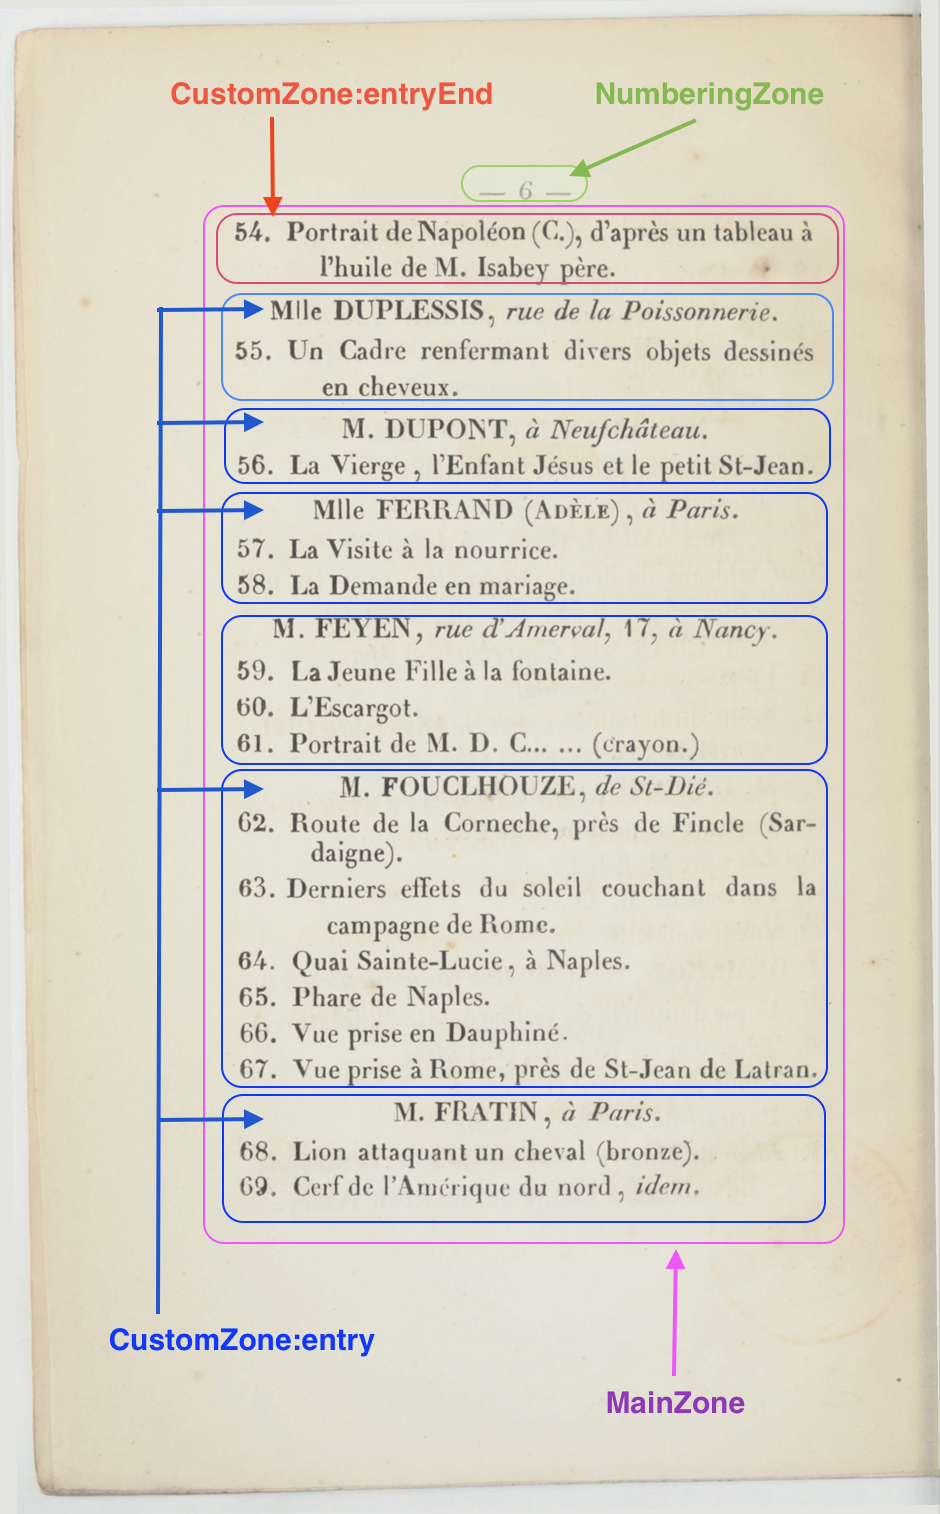
\includegraphics[scale=0.5]{exemples_zones.png}		
	\caption{Salon de Nancy 1843, p. 6.}
	\label{segmonto}
\end{figure}

Il faut que l'utilisateur prenne en compte et retienne∫ les éléments suivants :

\begin{itemize}
	\item Les Zones peuvent être parfois serrées, et il est important de veiller à ce qu'elles soient correctement imbriquées ou différenciées : la zone \texttt{NumberingZone} est extrérieure à la \texttt{MainZone} (espace sémantique), qui elle englobe toutes les \texttt{CustomZone:entry} et une \texttt{CustomZone:entryEnd}.
	
	\item Nous avons une \texttt{CustomZone:entryEnd} : c'est à dire une entrée coupée qui commence à la page antérieure (cela est évident dès lors qu'on ne voit pas de personne indiquée). Il est important de signaler ce type de zones pour que le script comprenne qu'il faut l'unir à la dernière entrée de la page antérieure.
\end{itemize}

\begin{figure}[ht]
	\centering
	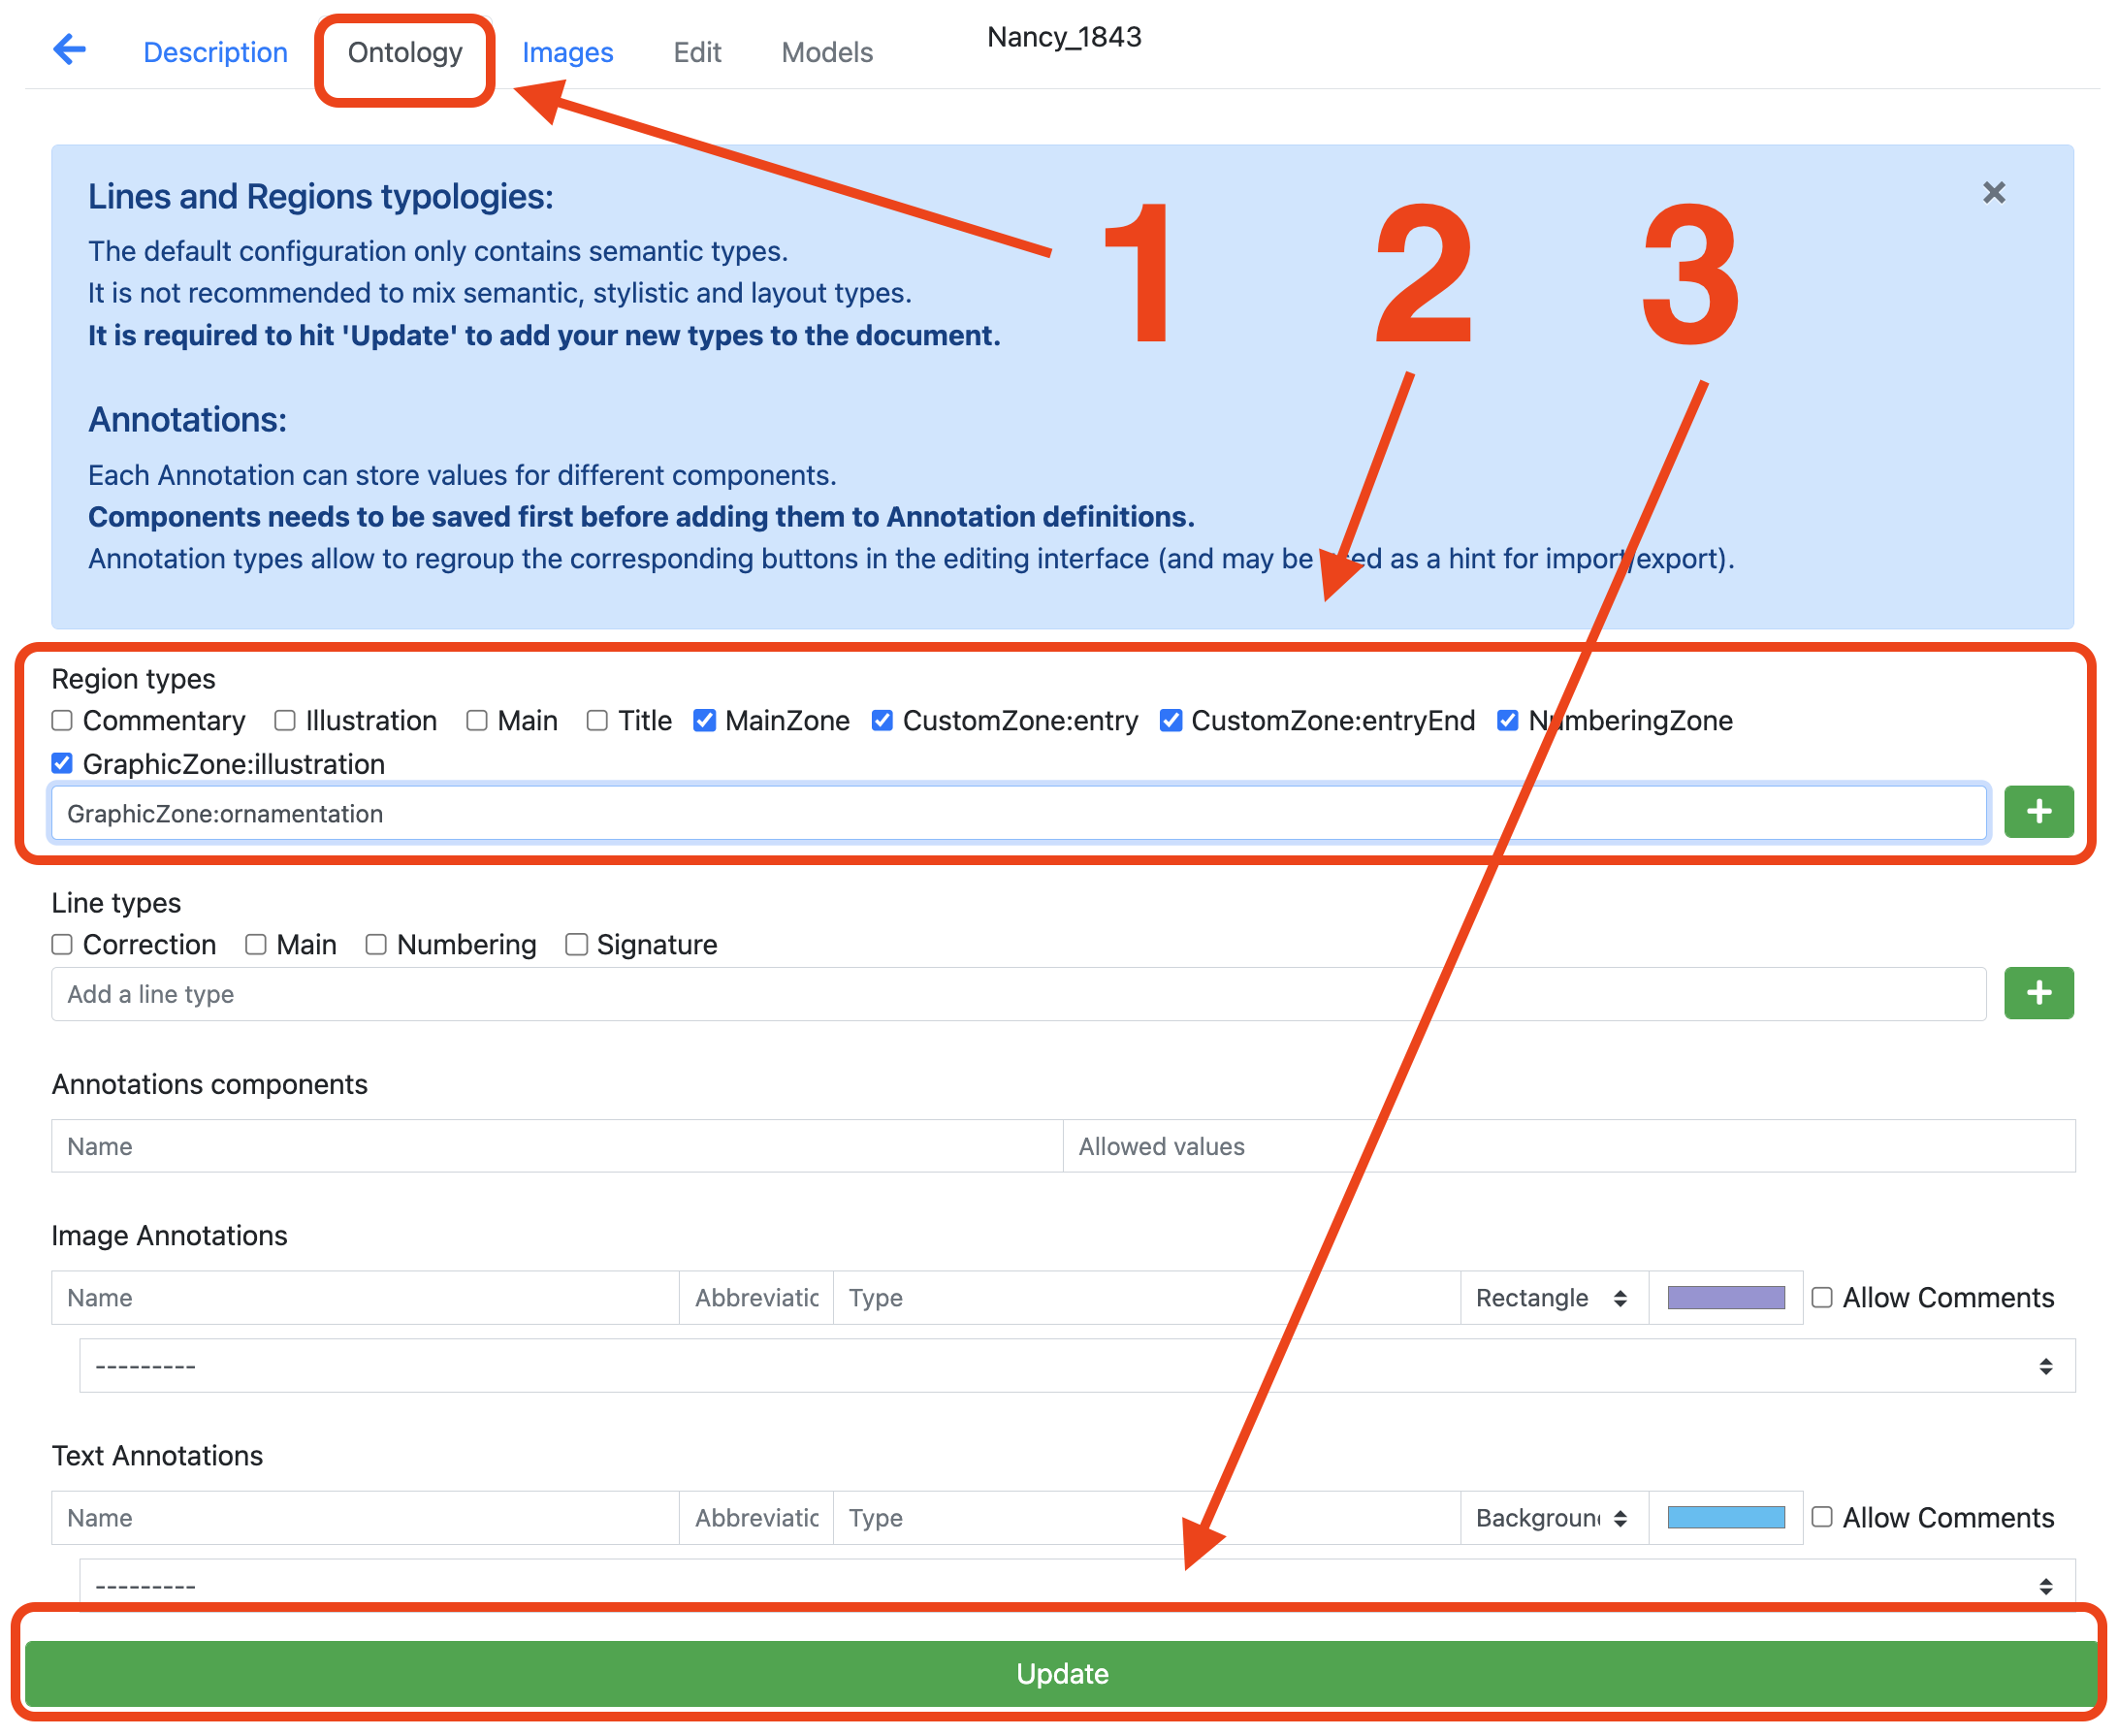
\includegraphics[scale=0.4]{ontologie_eScriptorium.png}		
	\caption{eScriptorium : Saisie des zones Segmonto}
	\label{saisiesegmonto}
\end{figure}

La figure \ref{saisiesegmonto} montre les étapes à suivre pour intégrer manuellement l'ontologie Segmonto au projet eScriptorium en cours. Il faut [1] aller sur l'onglet "Ontology" et saisir manuellement chaque zone de la manière suivante :
\begin{itemize}
	\item copier/coller chacune des zones sur la partie "Region types" et cliquer sur le bouton vert "+" (ajouter) [2]
		\item saisir une par une les régions, indiquées à continuation :
	\begin{itemize}
		\item \texttt{MainZone}
		\item \texttt{CustomZone:entry}
		\item \texttt{CustomZone:entryEnd}
		\item \texttt{NumberingZone}
		\item \texttt{GraphicZone:illustration}
		\item \texttt{GraphicZone:ornamentation}
	\end{itemize} 

	\item une fois toutes les régions saisies comme sur l'image, 
	Il est très important de ne pas oublier de cliquer sur le bouton \texttt{Update} [3]
\end{itemize}


Une fois cette saisie réalisée, les zones Segmonto pourront être appelées lors de l'étape postérieure de segmentation manuelle. 


\subsection{Quelles images utiliser ? Le standard iiif et les fichiers images classiques (jpeg, png, pdf)}

eScriptorium permet d'utiliser les principaux types de fichier image pour réaliser les transcriptions. Il est donc possible d'utiliser des formats communs tels que \texttt{.jpeg}, \texttt{.png} et \texttt{.pdf}. Cela suffira au programme extractionCatalogs pour fonctionner.

Cependant, le projet Artl@s préconise l'utilisation du standard iiif, qui est implémenté également par eScriptorium. iiif\footcite{IIIfInternationalImage} (International Image Interoperability Framework) est un standard de partage et de gestion des images privilégié dans le domaine des humanités numériques. Il permet d'exploiter et de faire circuler efficacement des images numériques de haute qualité entre institutions patrimoniales, universités et chercheurs. La prise en main des outils iiif nécessite un apprentissage technique qui ne sera pas requis dans le cadre de ce pipeline ; mais il est pertinent de mentionner l'existence de cette technologie aux étudiants, et sur un plan purement technique, cela est plus facile pour l'utilisateur. 

De plus, lorsque des images iiif sont utilisées, le script extractionCatalogs est capable de les découper, à partir des informations fournies dans le fichier ALTO sur la position des zones. Lorsque le catalogue transcrit sur eScriptorium provient d'un lien iiif, l'extraction sur le terminal intègre un lien vers l'image découpée de chaque entrée. C'est le cas pour le catalogue du Salon de Nancy 1843 donné en exemple, qui ayant été numérisé par la Bibliothèque nationale de France, provient de Gallica et est conforme au standard iiif. 

\begin{wrapfigure}{r}{0.20\textwidth}
	\centering
	
\includegraphics[width=0.20\textwidth]{iiif}
	\caption{Icône iiif}
	\label{iiif}
\end{wrapfigure}
Dans le cadre du pipeline extractionCatalogs, l'utilisation de catalogues conformes au standard iiif est extrêmement simple. Souvent, dans ces cas, le site source fournira l'icône iiif (voir figure \ref{iiif}). S'il existe, il devrait permettre de retrouver facilement un lien vers le "manifeste iiif" du document. Celui-ci est un fichier \texttt{.json} contenant des liens vers les images du catalogue ainsi que diverses métadonnées pour le reconstituer dans son ensemble. Dans le cas du catalogue de Nancy 1843, la figure \ref{trouver} montre comment le trouver.

\begin{figure}[ht]
	\centering
	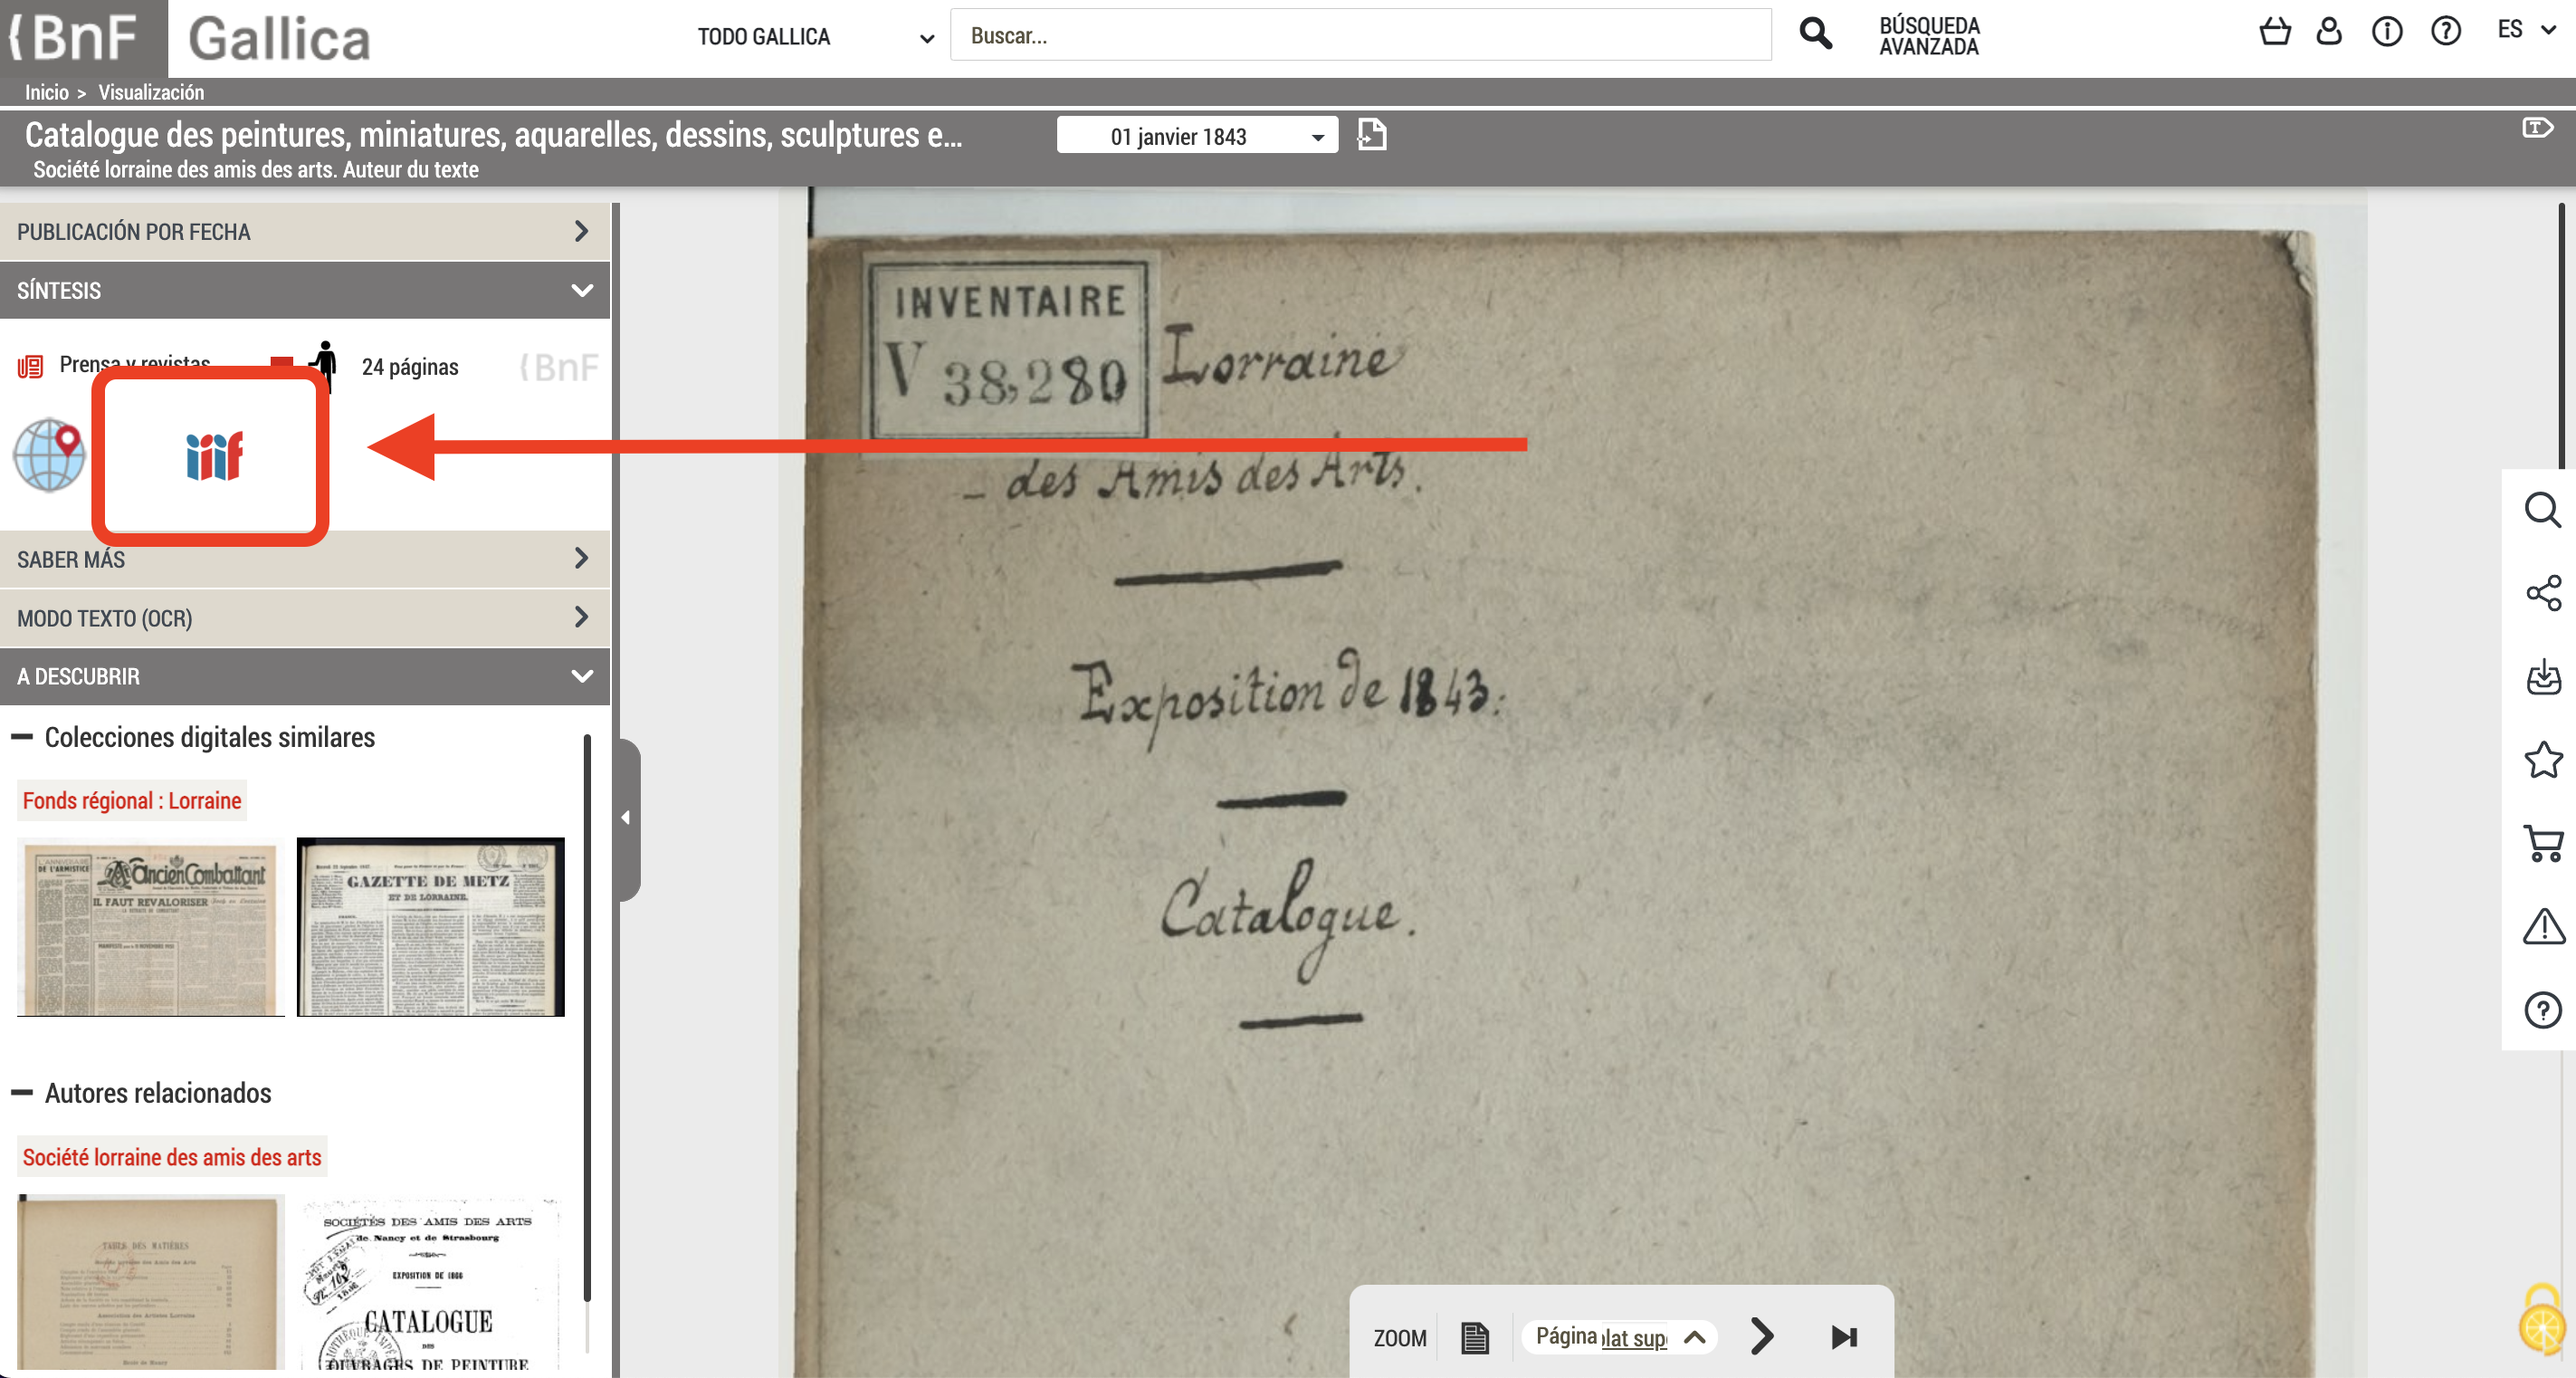
\includegraphics[scale=0.3]{lien_iiif.png}		
	\caption{iiif sur Gallica}
	\label{trouver}
\end{figure}

En cliquant sur cette icône, nous accédons à un "viseur iiif", c'est un dire un viseur capable de reconstituer un document visuel à travers des informations fournies par un manifeste iiif. Pour récupérer le manifeste iiif qu'il utilise, il faut [1] cliquer sur l d'information, puis [2] scroller jusqu'à la fin, comme indiqué sur la figure \ref{scroller}.

\begin{figure}[ht]
	\centering
	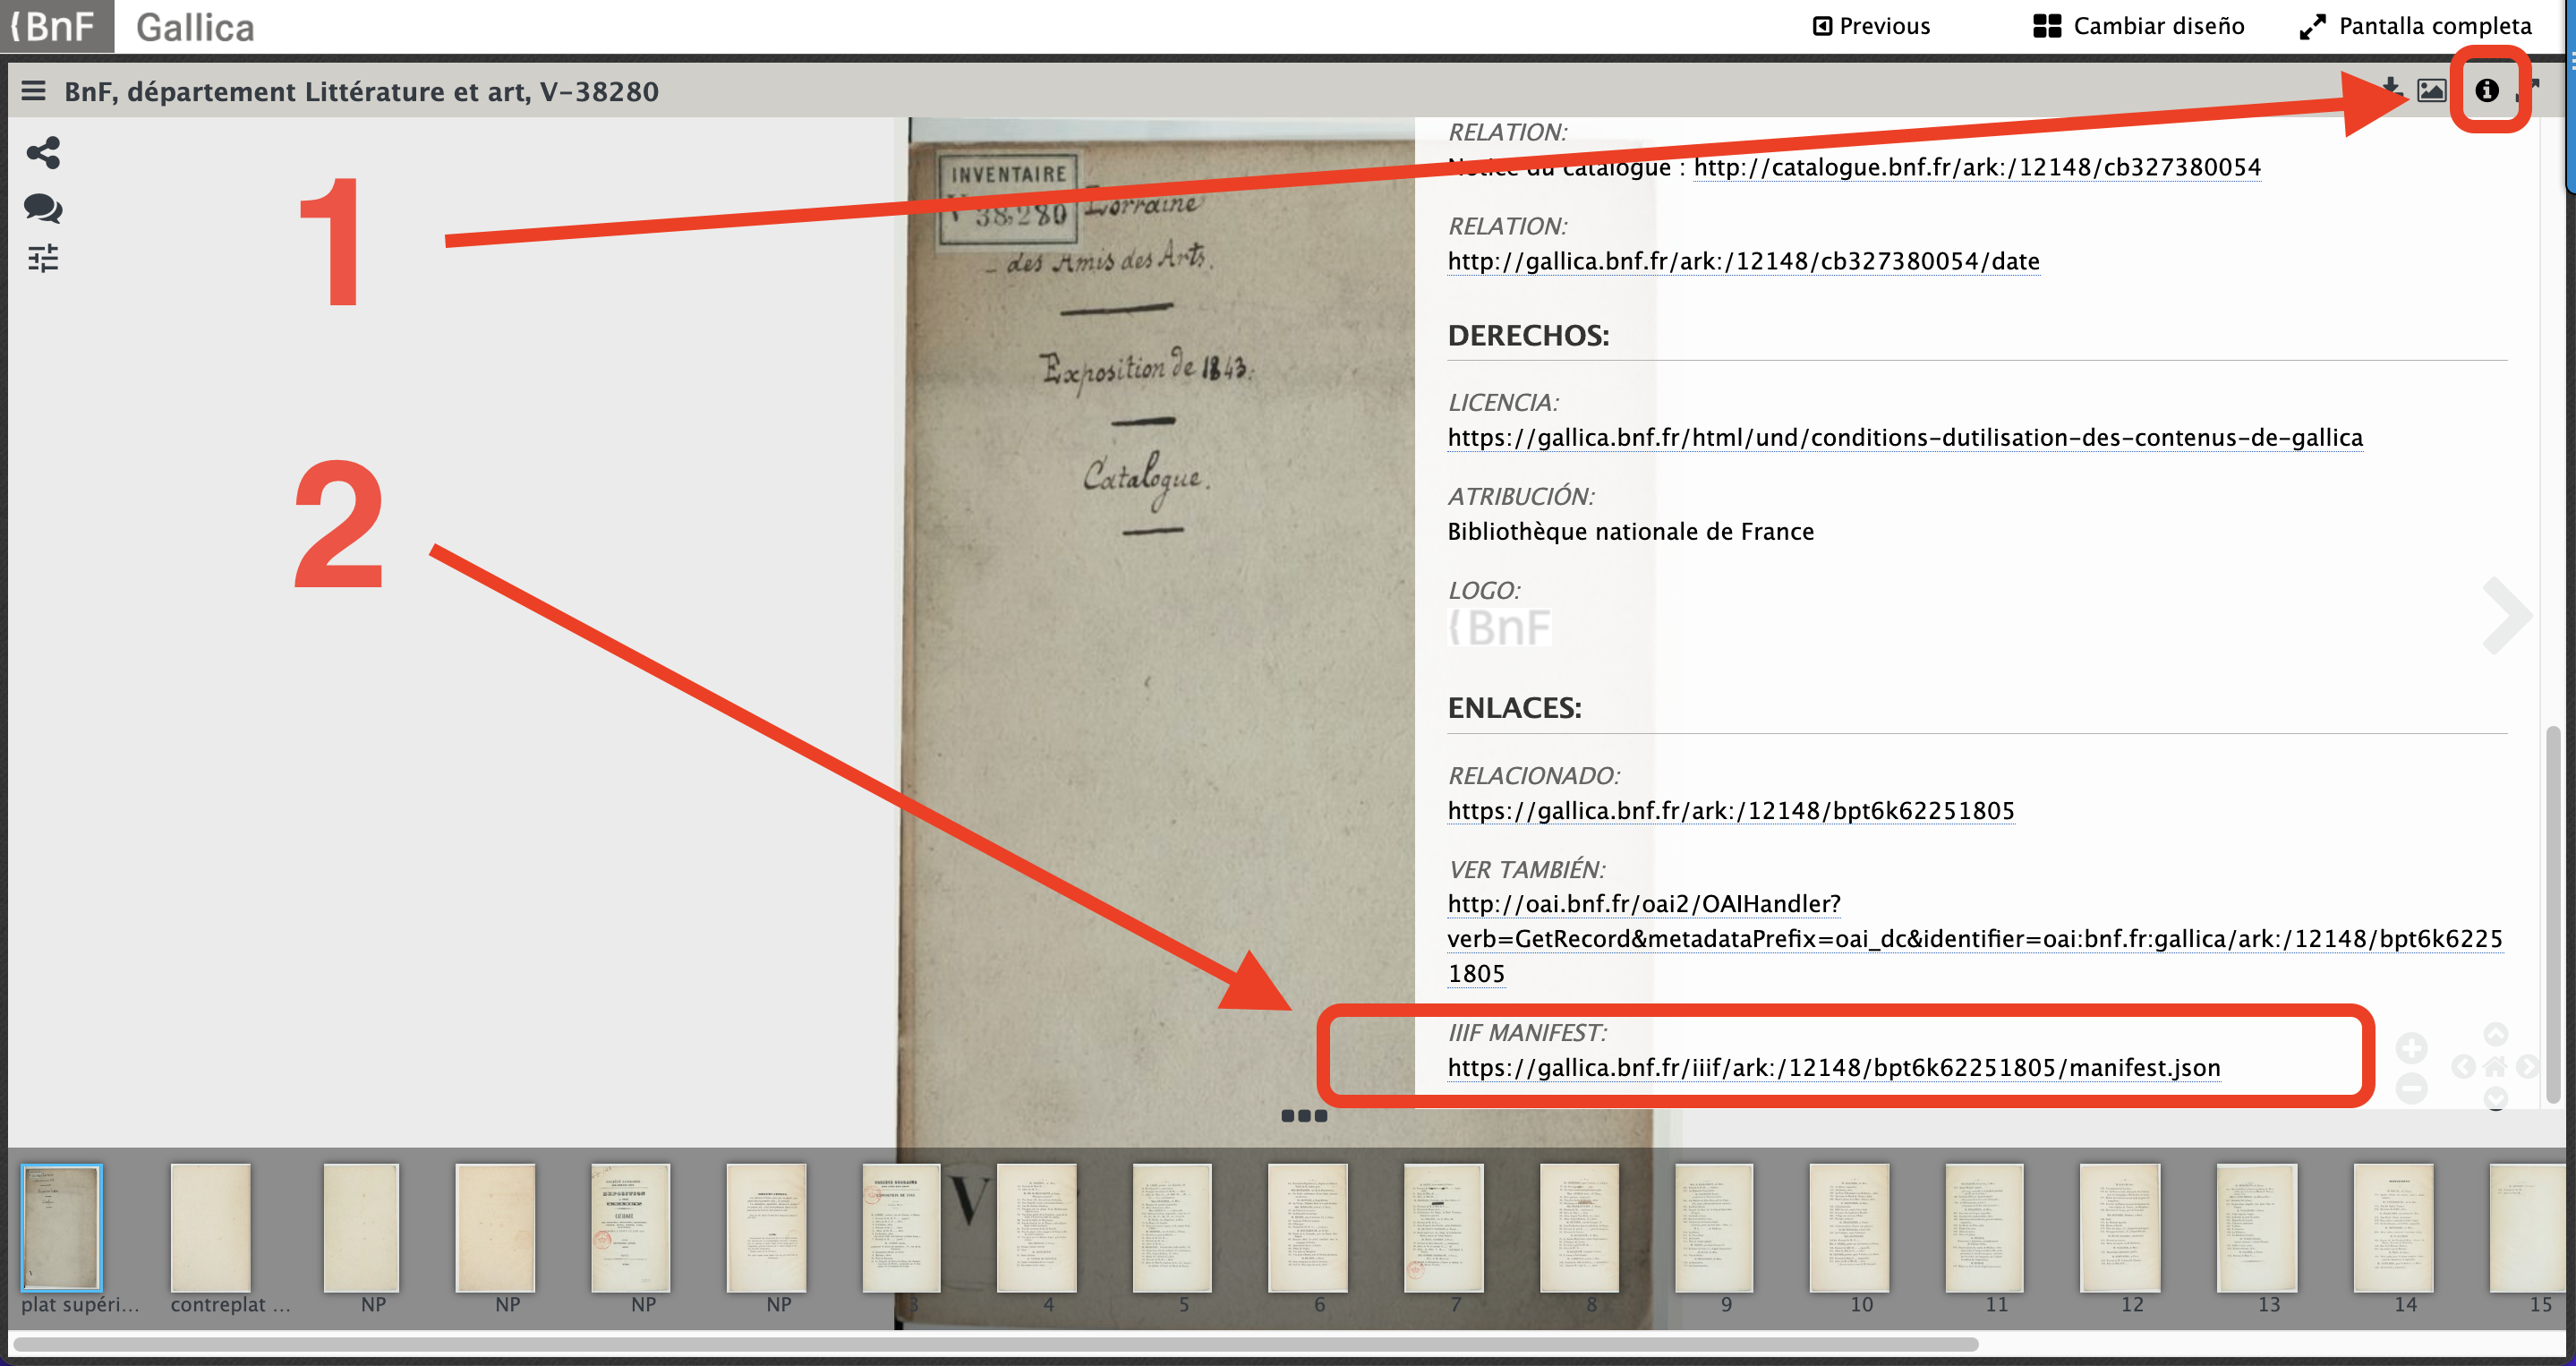
\includegraphics[scale=0.3]{lien_manifest.png}		
	\caption{Manifeste iiif sur Gallica}
	\label{scroller}
\end{figure}

On obtient ainsi le lien suivant :

\mint{bash}|https://gallica.bnf.fr/iiif/ark:/12148/bpt6k62251805/manifest.json|

Ce lien mène vers le manifeste iiif écrit en langage \texttt{.json}. Ce liens sont faciles à reconnaître car ils se terminent toujours par la chaîne \texttt{manifest.json}. Il suffit à l'utilisateur de copier/coller ce lien sur eScriptorium au moment de saisir les images. 


\subsection{Ajouter des images (iiif, jpeg, png, pdf, etc.)}

La figure \ref{ajout} montre comment ajouter les images au document courant sur eScriptorium. Il faut [1] Cliquer sur l'onglet "Images" et choisir une option qui convienne au format des images en \texttt{input} :
\begin{itemize}
	\item [2.1] Déposer des fichiers images une par une (\texttt{.jpg}, \texttt{.png}, etc.)
	\item [2.2] Cliquer sur \texttt{Import} puis sur IMAGES (IIIF), puis coller un lien vers les manifeste iiif du catalogue. Cliquer sur \texttt{Start importing} : eScriptorium s'occupera d'importer toutes les images
	\item [2.3] Cliquer sur \texttt{Import} puis sur IMAGES (PDF), puis ajouter un document \texttt{.pdf} Cliquer sur \texttt{Start importing} :  eScriptorium s'occupera de le découper en images isolées.
\end{itemize}
\begin{figure}[ht]
	\centering
	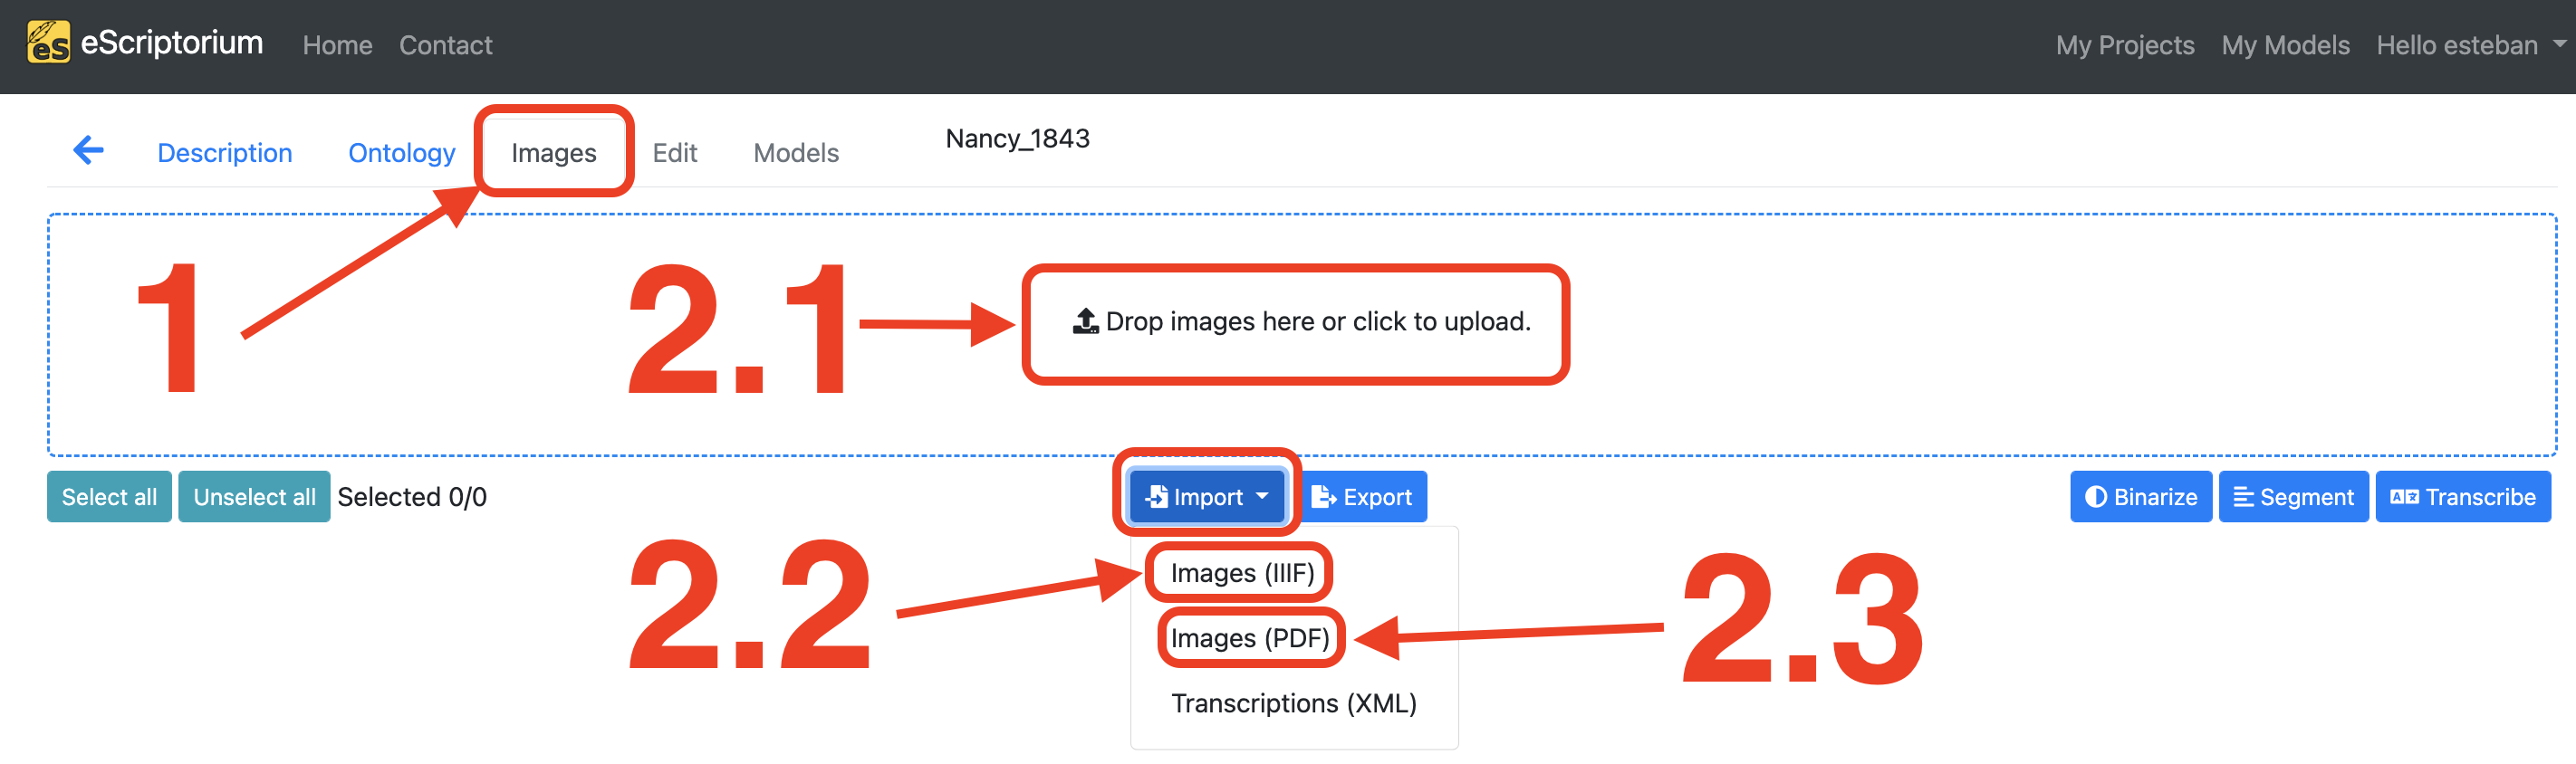
\includegraphics[scale=0.3]{ajouter_images_eScriptorium.png}		
	\caption{eScriptorium: choisir des images}
	\label{ajout}
\end{figure}

La figure \ref{frise} montre ce qui se passe dans le cas du catalogue de Nancy 1843 : on obtient une frise avec 24 images.

\begin{figure}[ht]
	\centering
	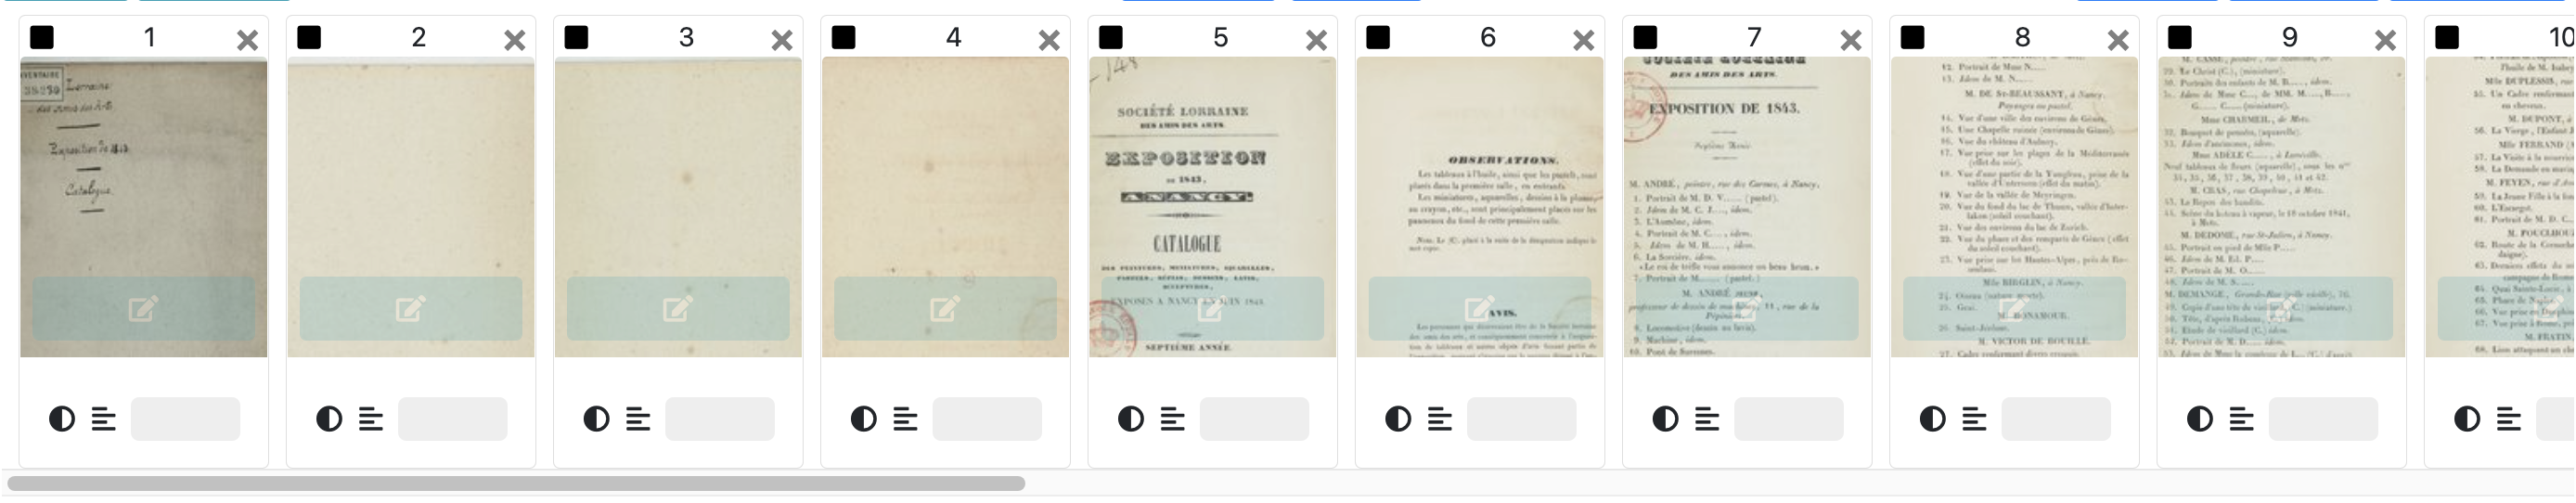
\includegraphics[scale=0.3]{frize_eScriptorium.png}		
	\caption{eScriptorium : frise d'images}
	\label{frise}
\end{figure}

Lors de l'utilisation du script extractionCatalogs, seules les pages contenant des entrées vont être traitées. Cela veut dire que seuls des fichiers qui contiennent des zones segmonto \texttt{CustomZone:entry} seront prises en compte. L'utilisateur est donc libre de conserver ou d'éliminer les images sans entrées avec la petite croix en haut à gauche de chaque image. Dans notre cas, nous choisissons de garder deux pages sans entrées, afin de montrer explicitement ce qu'il en sera lors du traitement avec le script. La frise comporte désormais 15 images, et les deux premières n'ont aucune entrée. 

\section{Transcription automatique des images}

Dans la frise d'images, nous pouvons observer des icônes individuels avec des boutons. La figure \ref{image} montre ce niveau et les manipulations fondamentales qu'il permet de réaliser :
\begin{enumerate}
\item Case pour sélectionner des ensembles d'images à traiter. Toutes les images dont cette case est coché subiront les mêmes traitements simultanément.
\item Éditeur d'image : renvoie vers la page d'édition, qui permet entre autres de saisir des transcriptions/segmentations manuelles, ou bien de corriger des transcriptions/segmentations automatiques. 
\item Bouton "binariser" : transforme l'image en tons de gris, ce qui facilite la reconnaissance de caractères. Nous avons pas besoin d'utiliser cette fonctionnalité
\item Bouton "segmenter" : permet de segmenter, c'est à dire de reconnaître des régions, mais aussi localiser les lignes dans la page. Dans notre cas, nous ferons usage uniquement de la reconnaissance automatique des lignes.
\item Bouton "transcrire" : permet d'appliquer un modèle de reconnaissance de caractères au choix, selon une liste proposée par eScriptorium.
\end{enumerate}
\begin{figure}[ht]
	\centering
	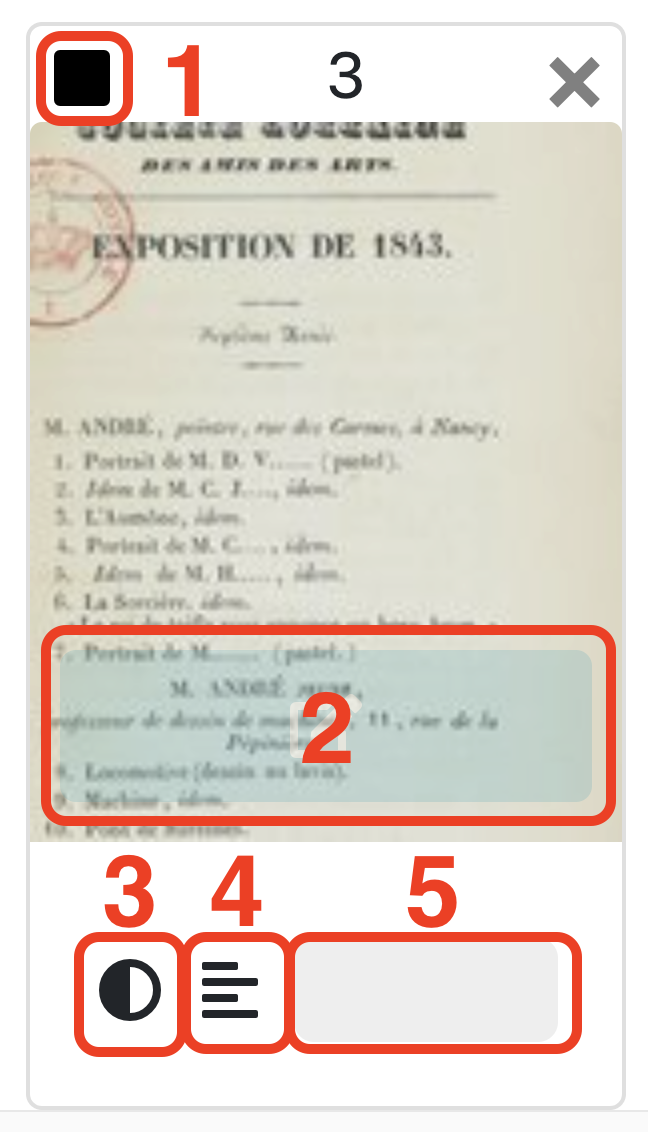
\includegraphics[scale=0.4]{icone_image_eScriptorium.png}		
	\caption{eScriptorium : icône image}
	\label{image}
\end{figure}

Il faut d'abord choisir les images à transcrire automatiquement en cochant sur elles. Pour aller plus vite, l'utilisateur peut maintenir les touches COMMAND/SHIFT appuyées et sélectionner la première et la dernière image : toutes les images entre les deux seront cochées automatiquement. Dans le cas du catalogue Nancy 1843, nous allons cocher toutes sauf la première (page de titre), ce qui laisse 14 images, dont une (numéro 2) sans entrées (voir figure \ref{cochees}). C'est le cas d'usage pour mettre de côté des images non concernées importées automatiquement à partir d'un manifeste iiif. 
Maintenant, si on appuie sur n'importe quel bouton de n'importe quel icône, l'ensemble des images cochées subiront le même traitement.
 
\begin{figure}[ht]
	\centering
	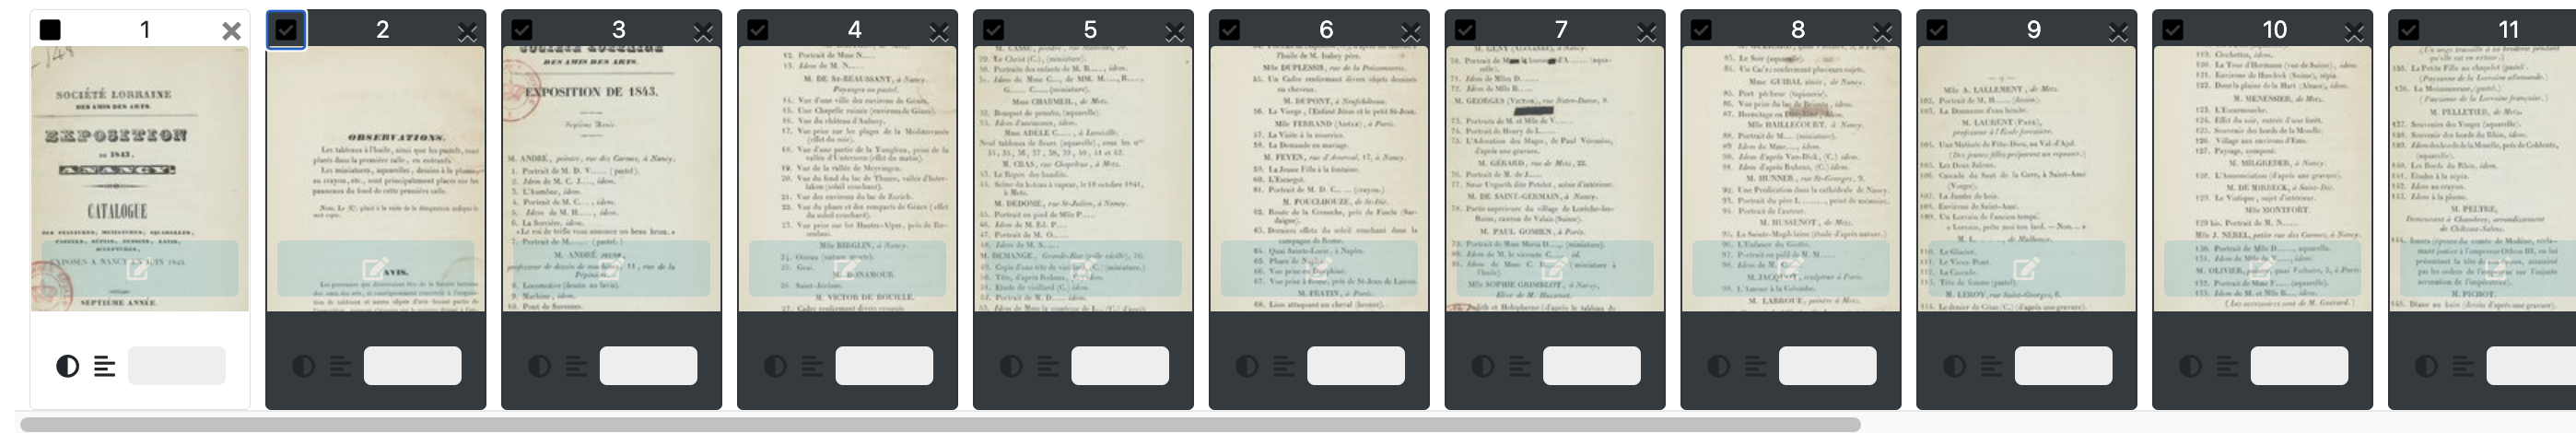
\includegraphics[scale=0.3]{cocher_eScriptorium.png}		
	\caption{eScriptorium : sélection d'images dans la frise}
	\label{cochees}
\end{figure}

La première étape consiste à utiliser la fonctionnalité de segmentation automatique, non pas pour reconnaître des régions, mais pour reconnaître des lignes à transcrire. Comme indiqué sur la figure \ref{lignes}, il faut [1] cliquer sur n'importe quel bouton "segmenter" d'une des images cochées, ou bien sur le bouton général "Segment". Puis [2] sélectionner l'option "Lines Baselines and Masks" (et surtout pas l'option par défaut "Lines and regions", puisque la segmentation des régions sera faite manuellement). Pour terminer, il faut [3] cliquer sur "Segment". Une fois une image segmentée, son bouton "segmenter" devient vert.
\begin{figure}[ht]
	\centering
	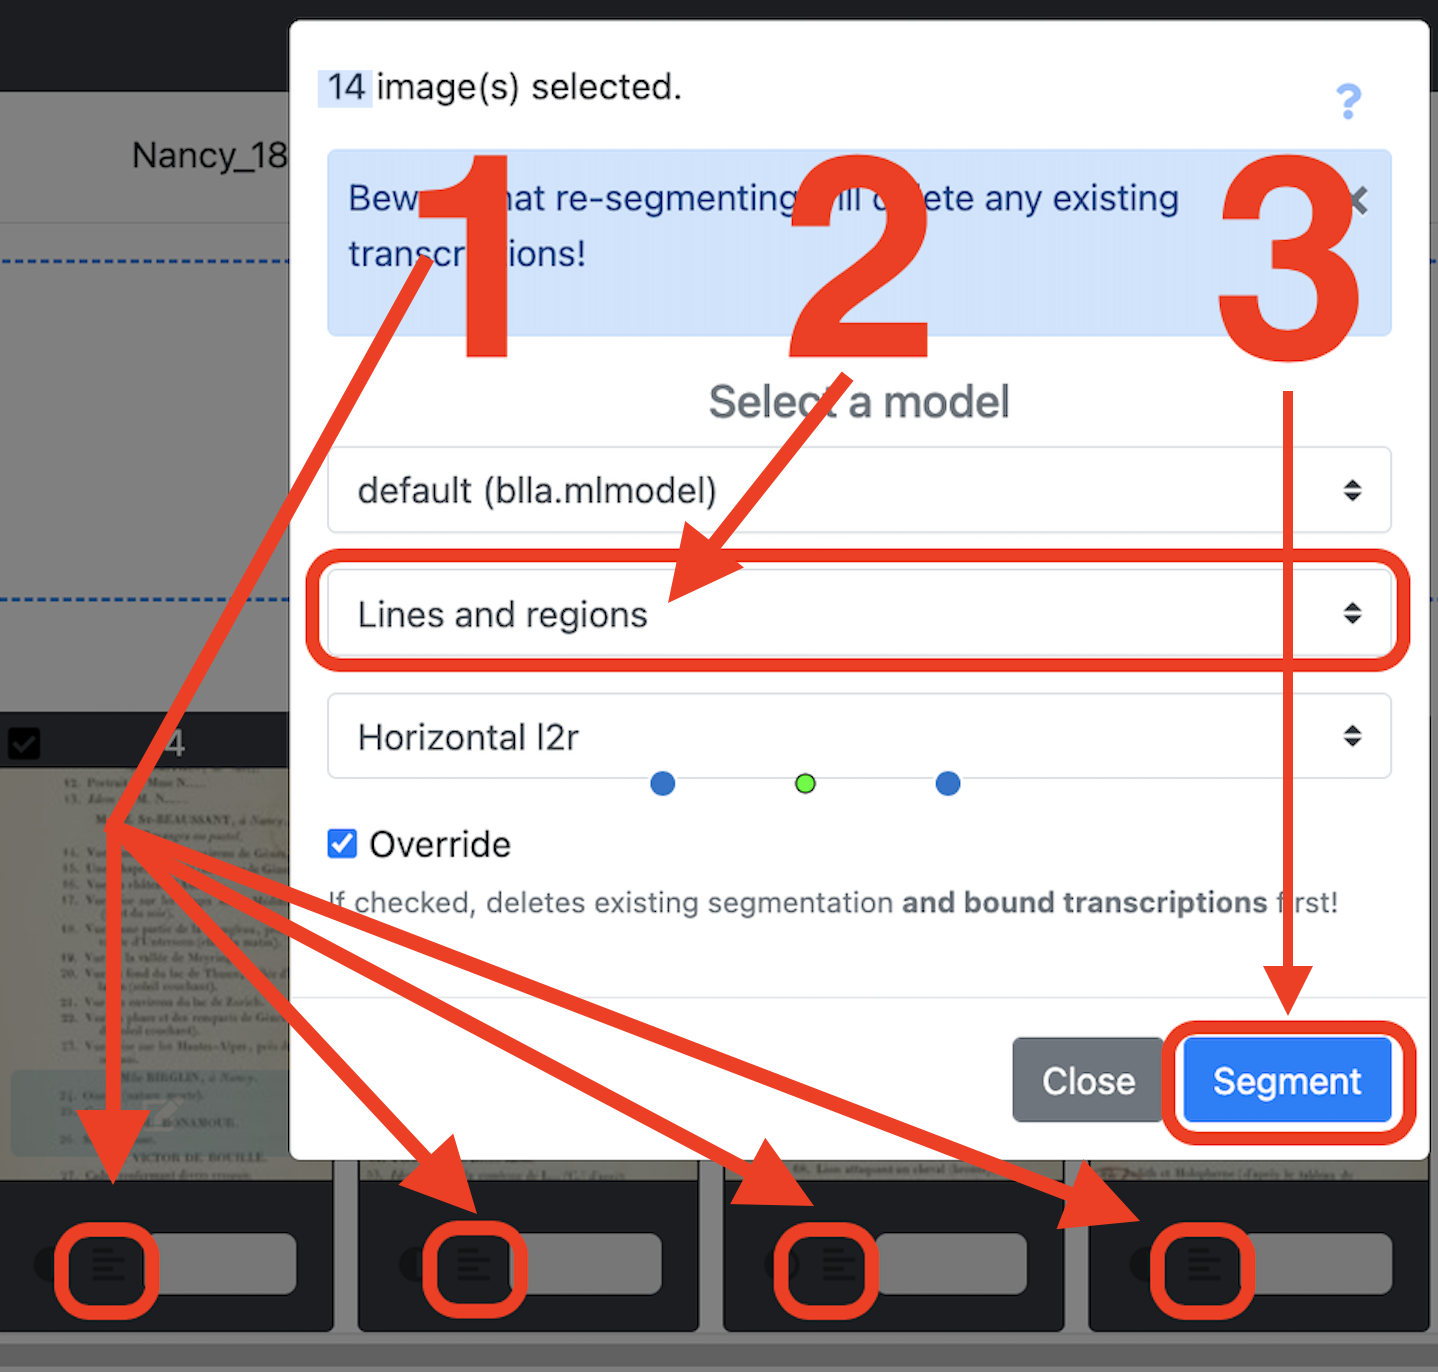
\includegraphics[scale=0.3]{lines_eScriptorium.png}		
	\caption{eScriptorium : reconnaissance des lignes}
	\label{lignes}
\end{figure}

L'étape suivante consiste à lancer une transcription automatique du texte contenu dans les images. Comme indiqué sur la figure \ref{transcrire}, l'utilisateur doit [1] cliquer sur n'importe quel bouton "transcrire" d'une des images cochées, ou bien sur le bouton général \texttt{Transcribe}. Il faut après [2] sélectionner le modèle "19th Century prints - HTRcatalogs Artlas" (ou bien celui du choix de l'utilisateur). Finalement, il faut [3] cliquez sur \texttt{Transcribe}. Une fois une image transcrite, son bouton "transcrire" indique la complétion à \texttt{100\%}. 
\begin{figure}[ht]
	\centering
	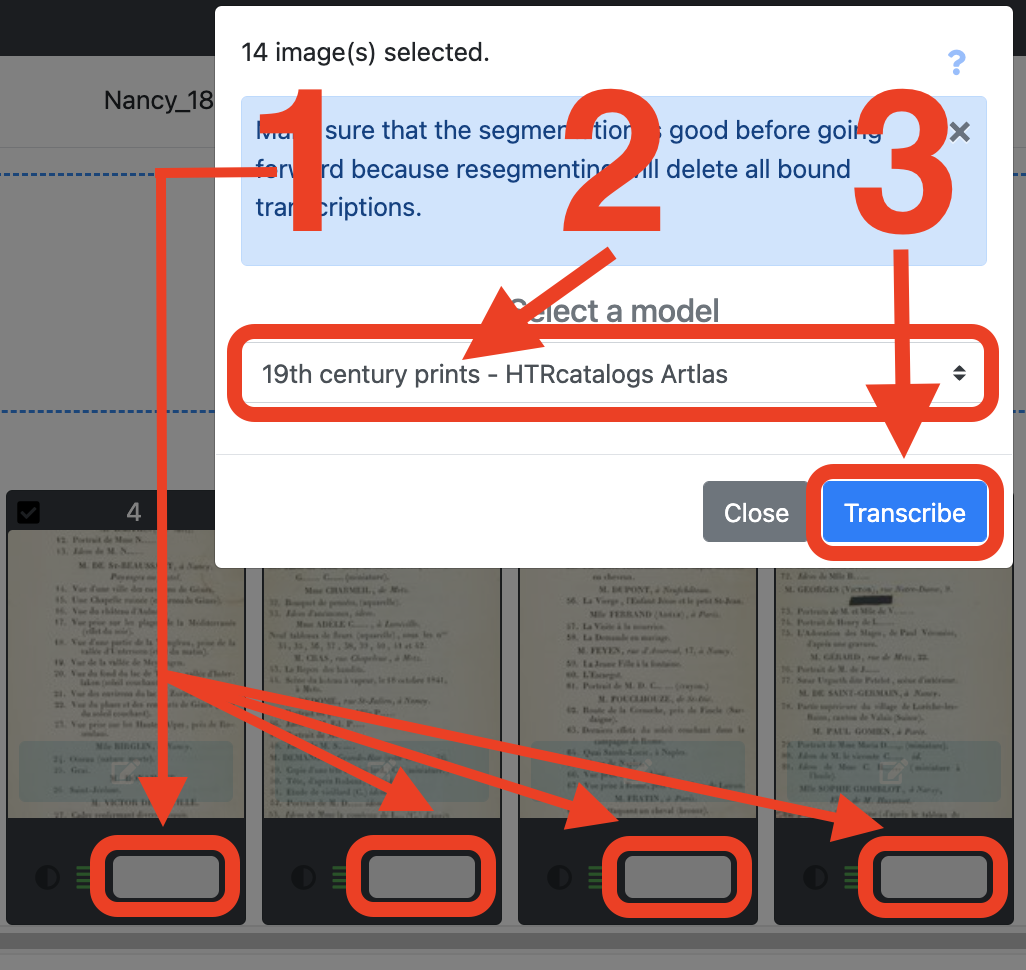
\includegraphics[scale=0.4]{transcribe_eScriptorium.png}		
	\caption{eScriptorium : lancer la transcription}
	\label{transcrire}
\end{figure}

L'utilisateur peut à présent consulter et éditer les transcriptions en cliquant sur le bouton "éditer" des icônes ; il le mènera vers la page d'édition de chaque image, où il pourra corriger manuellement la transcription automatique, puis segmenter manuellement les régions.

\begin{figure}[ht]
	\centering
	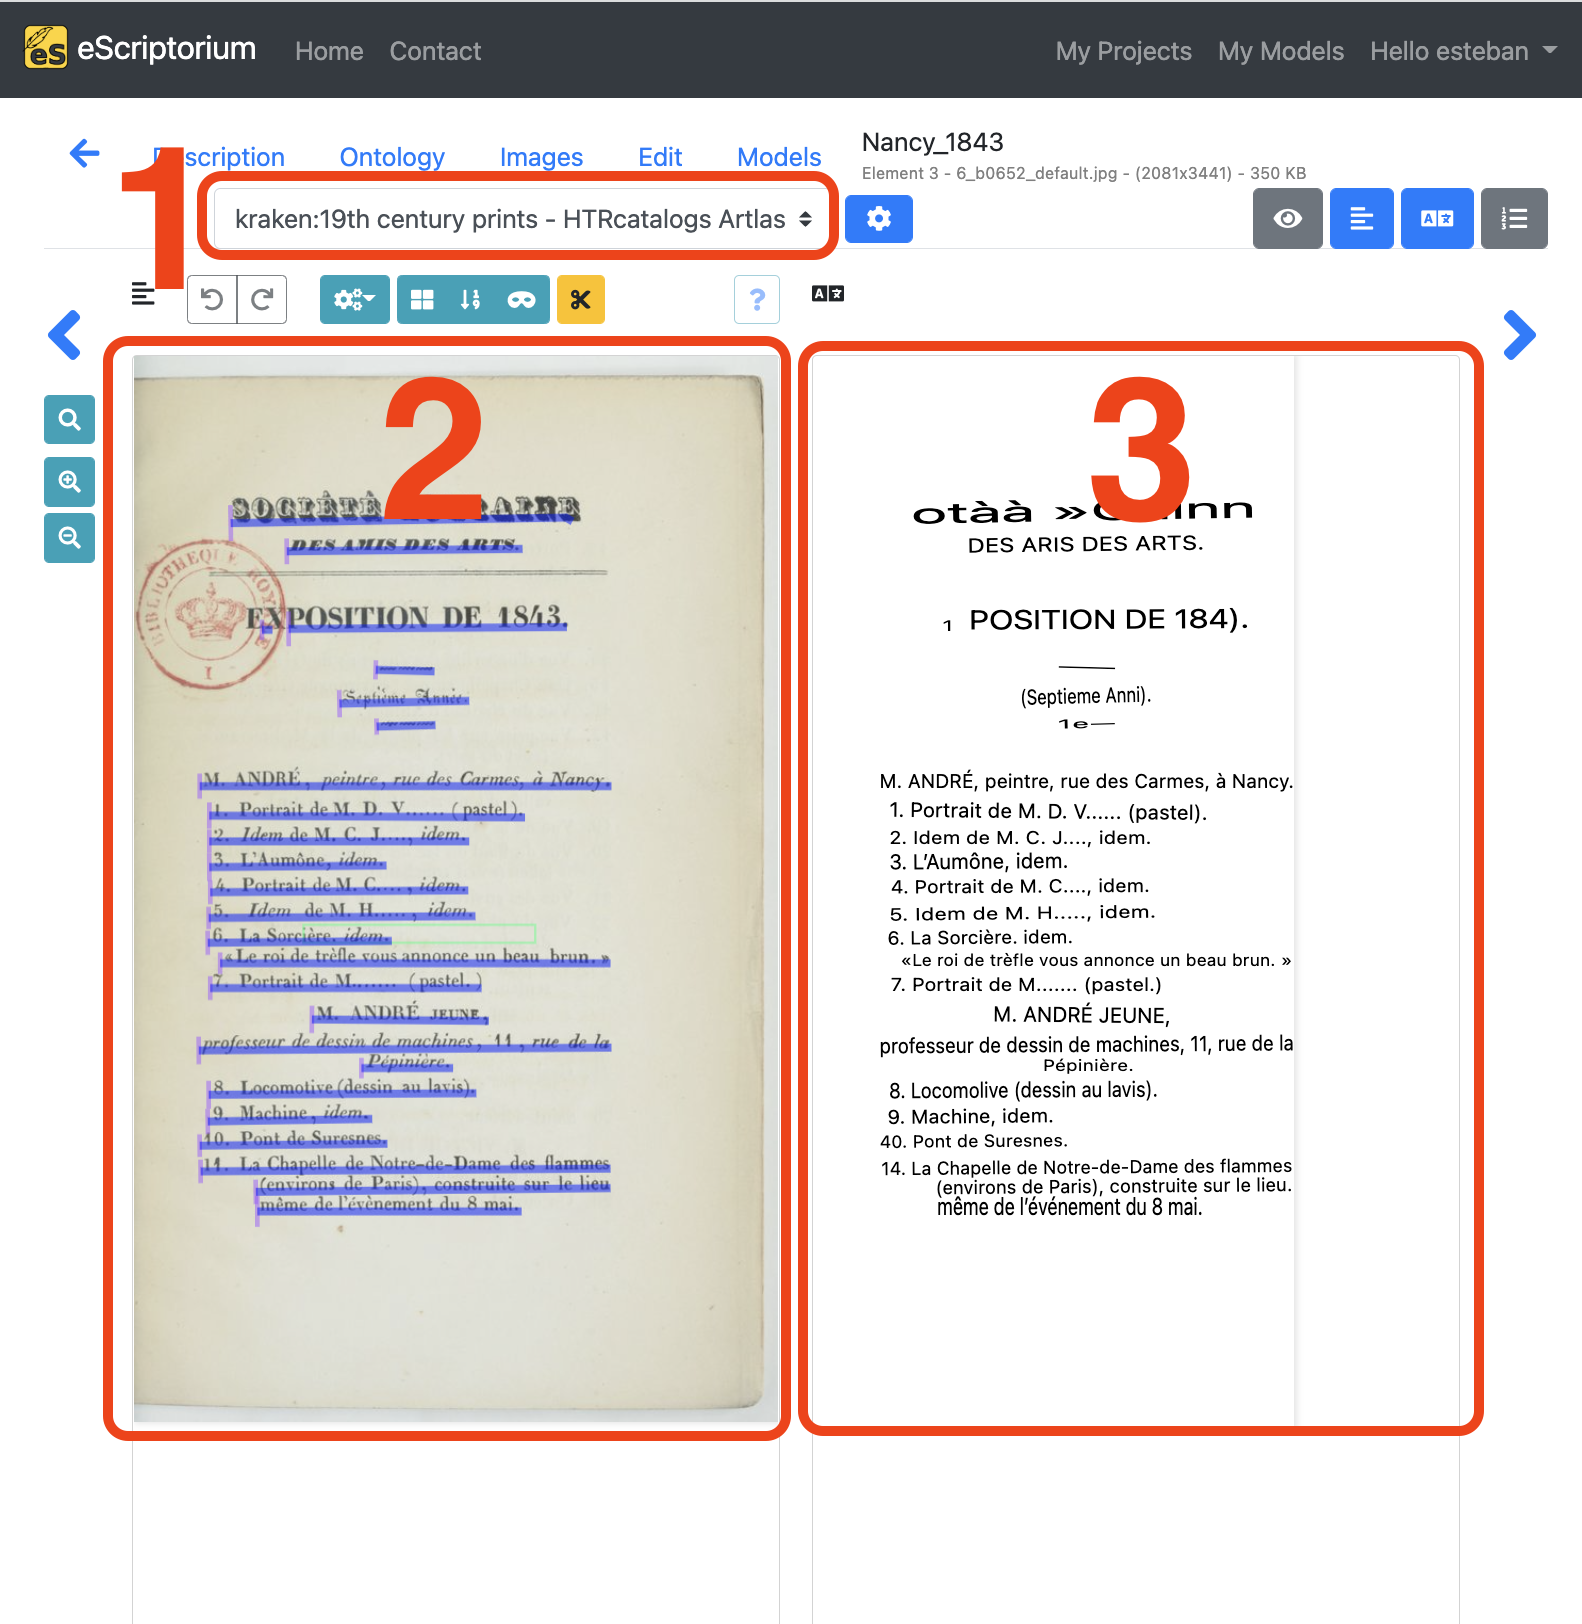
\includegraphics[scale=0.3]{editer_eScriptorium.png}		
	\caption{eScriptorium : page d'édition}
	\label{pageedition}
\end{figure}
Comme indiqué sur la figure \ref{pageedition}, pour que la transcription s'affiche correctement, il faut [1] choisir la transcription qui correspond au modèle de reconnaissance de caractères choisi. Sur le viseur de la transcription, on trouvera à gauche [2] l'image courante, avec la segmentation des régions et des lignes (si ces segmentations existent), et à droite [3] la transcription du texte contenu dans l'image (si elle existe). 


Pour corriger la transcription (voir figure \ref{corriger}), l'utilisateur doit [1] cliquer sur la ligne qu'il souhaite corriger dans la section "transcription" (à droite), puis [2] écrire le texte souhaité sur l'éditeur qui apparait. Le catalogue Nancy 1843 fournit un bon exemple d'une transcription non satisfaisante, puisque le texte "SOCIÉTÉ LORRAINE" a été très mal reconnu. Cela est normal, puisqu'il ne s'agit pas de caractères typiques :
\begin{figure}[ht]
	\centering
	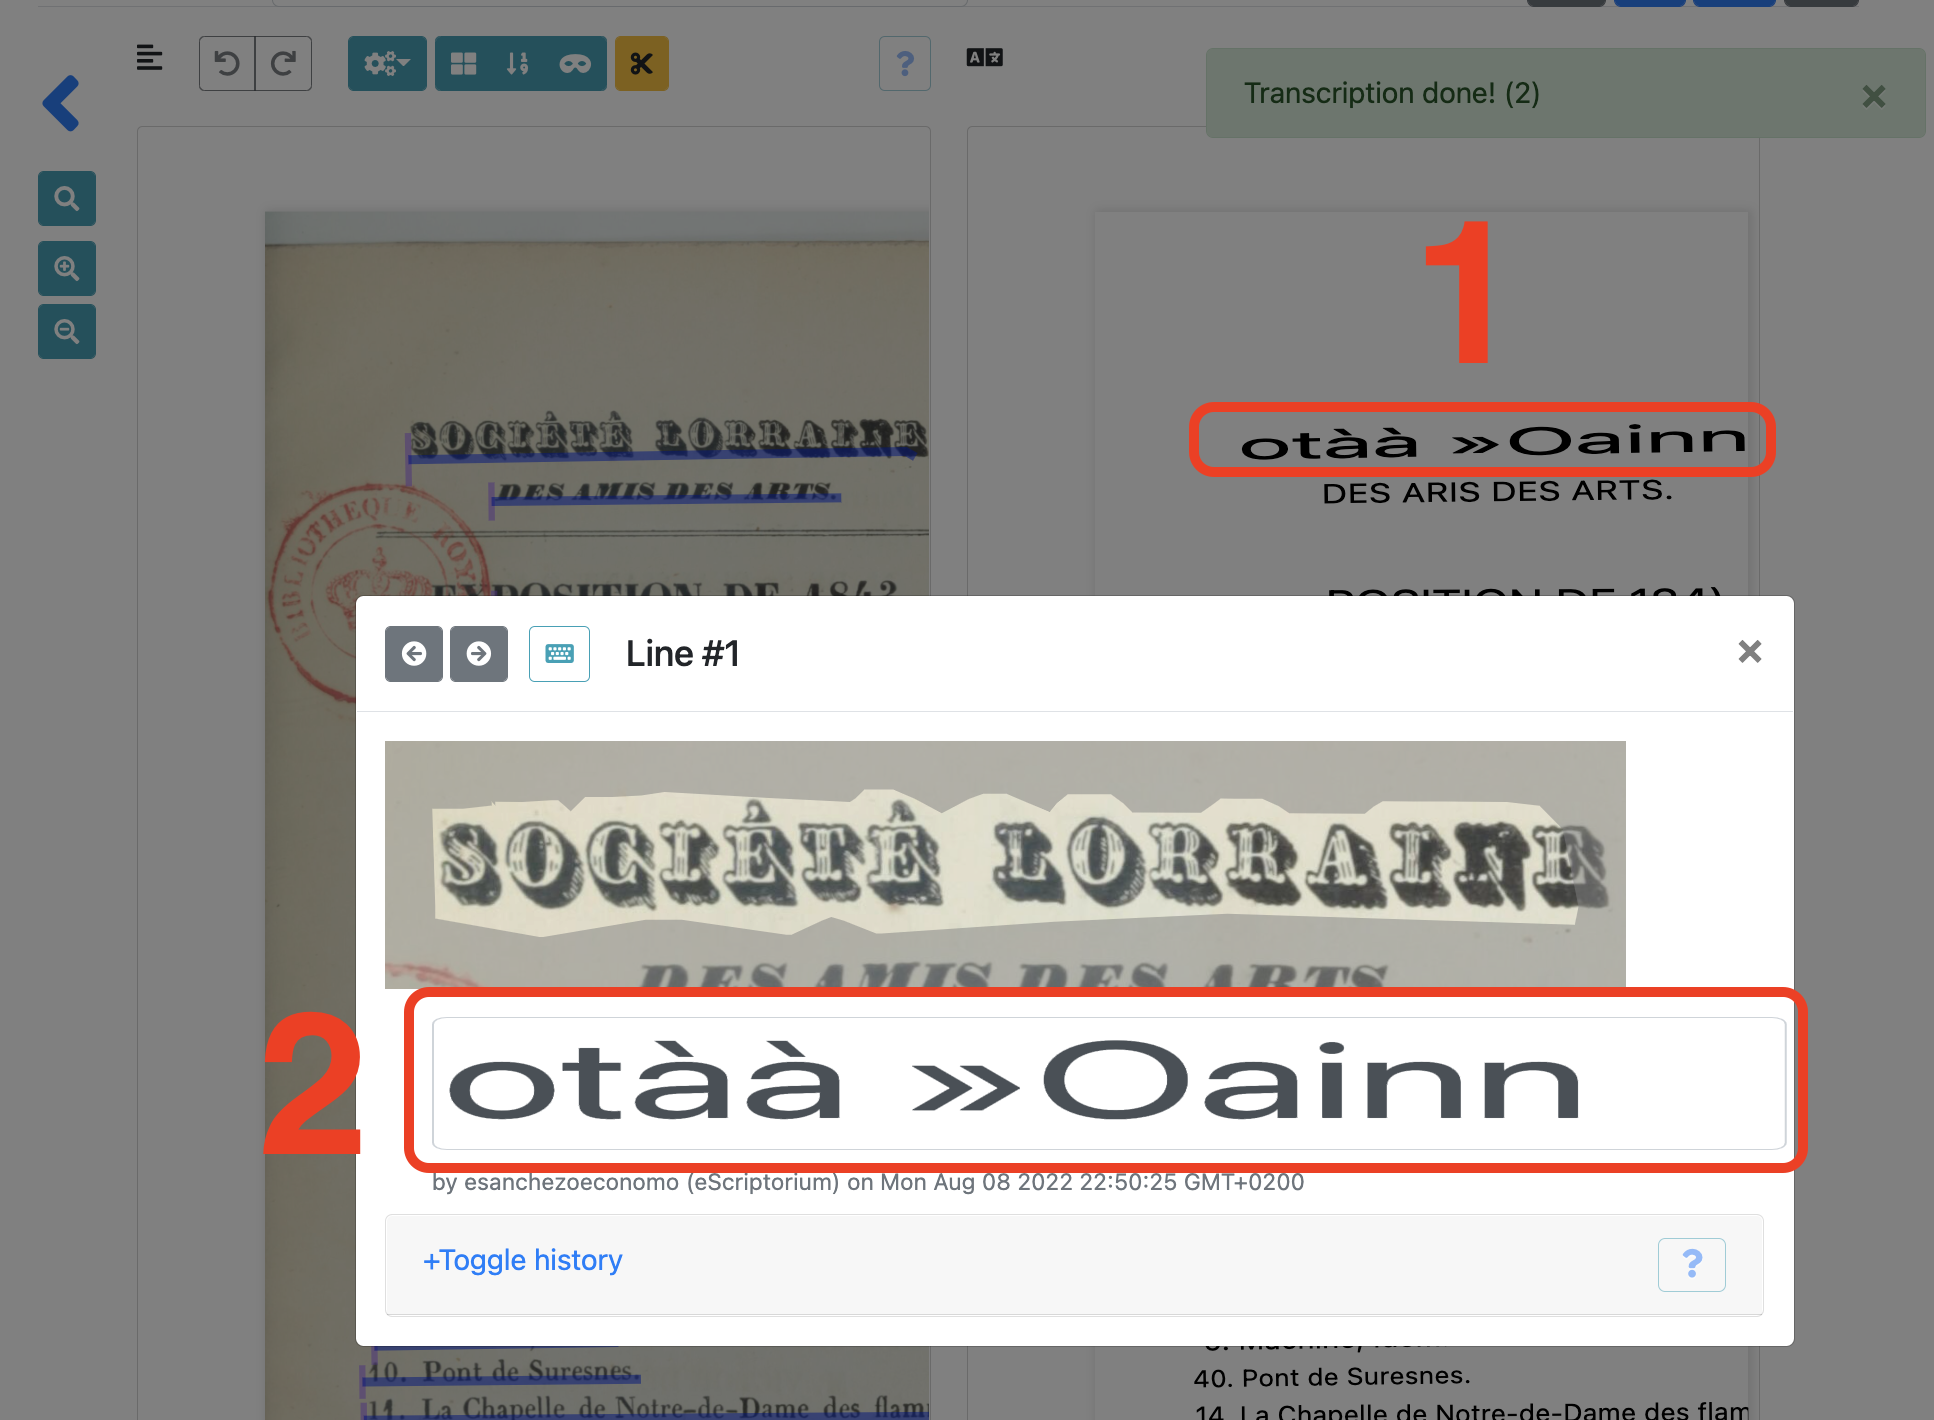
\includegraphics[scale=0.3]{corriger_eScriptorium.png}		
	\caption{eScriptorium : corrections manuelles}
	\label{corriger}
\end{figure}

Il suffit alors de substituer la correction au texte affiché, puis de  cliquer sur ENTER ou sur le bouton de flèche vers le bas afin d'aller vers la ligne suivante. L'utilisateur doit vérifier chaque ligne de chaque page, et faire toutes les corrections nécessaires. Il est important que les ponctuations soient correctement transcrites, et en particulier les caractères qui signalent des œuvres (par exemple "1. titre de l'œuvre"). Il faut vérifier les numéros, mais aussi les points et les tirets qui délimitent le numéro et le titre de l'œuvre, les virgules qui séparent les numéros des adresses, etc. ; ces éléments sont importants pour que le script soit capable de reconnaître des sections différentes pour reconstituer les entrées du catalogue. L'utilisateur n'a pas besoin de sauvegarder ses corrections, cela se fait automatiquement au fur et à mesure des modifications.

\section{Segmentation manuelle des images}

Une fois la correction de la transcription automatique terminée, l'utilisateur peut faire la segmentation manuelle des images. Cela se passe dans la section de gauche, qui contient l'image de la page. Cette section sert à signaler sur la page des régions et des lignes détectées automatiquement ou saisies manuellement. 

Par défaut, en cliquant sur l'image, l'utilisateur dessine des lignes. Il peut (et parfois doit) modifier des lignes qui sont mal saisies ou détectées. La figure \ref{lignesproblemes} inclut les cas les plus communs : elles peuvent [1] ne pas couvrir tout le texte, [2] déborder des régions, ou [3] couvrir des espaces où il n'y a pas de texte. Il est possible de les manipuler en cliquant dessus, ou des les éliminer en cliquant dessus puis sur le bouton rouge "poubelle" à gauche de l'image.

\begin{figure}[ht]
	\centering
	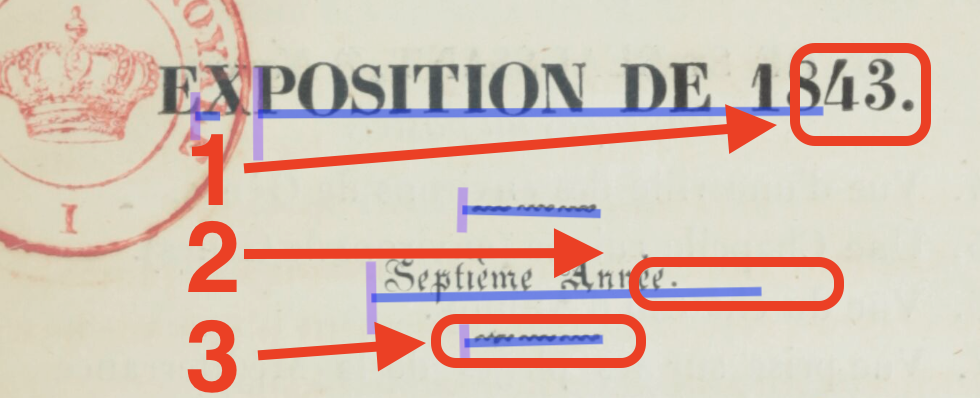
\includegraphics[scale=0.5]{lignes_eScriptorium.png}		
	\caption{eScriptorium : lignes avec erreurs}
	\label{lignesproblemes}
\end{figure}

La figure \ref{regions} montre comment dessiner des régions. L'utilisateur doit [1] cliquer sur le bouton "Switch to region mode", puis [2] saisir la région sur l'image avec la souris. Il faut aussi indiquer le nom de la zone :  il faut [3] cliquer sur le bouton "T", puis [4] sélectionner la zone concernée et appuyez sur ENTER. C'est ici que l'ontologie Segmonto, saisie précédemment, est affichée et disponible pour le nommage des zones.
\begin{figure}[ht]
	\centering
	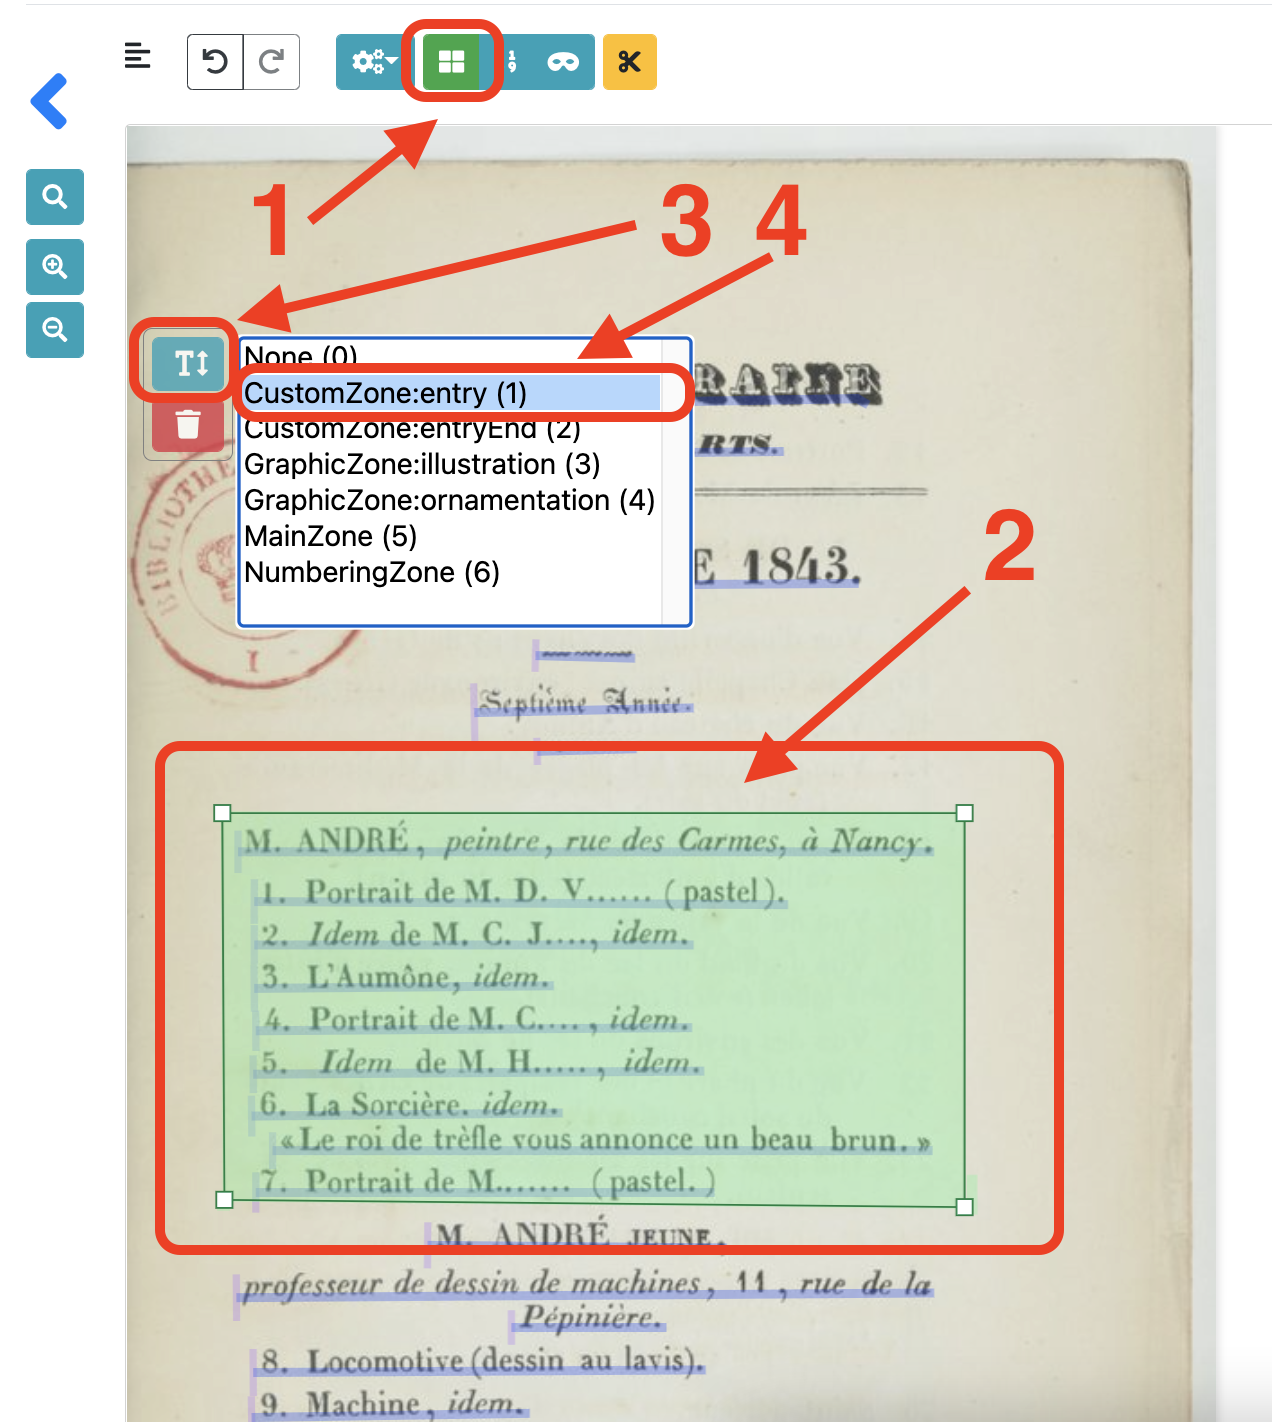
\includegraphics[scale=0.4]{regions_eScriptorium.png}		
	\caption{eScriptorium : saisir des zones}
	\label{regions}
\end{figure}

Normalement, l'ordre de saisie des régions aura un impact sur l'imbrication des éléments dans le fichier ALTO en \texttt{output}. Cela posait problème et impliquait que tout document saisi dans un ordre différent à celui compris par le script ne puisse être traité : avant notre mission, c'était le cas de la plupart des catalogues dans le corpus de transcriptions. \textsl{}Le script est actuellement capable de restructurer ces imbrications et de comprendre tous les documents ALTO en entrée, raison pour laquelle l'ordre de saisie des régions ne posera aucun problème. Il est tout de même important de faire noter à l'utilisateur cette situation, afin qu'il prenne conscience sur les bonnes pratiques de saisie des régions sur eScriptorium. Il faut commencer par les plus proches du texte, puis les plus amples et générales. Une fois les \texttt{CustomZone:entry}, \texttt{CustomZone:entryEnd} et \texttt{NumberingZone} saisies (ou tout autre type de zone), il faudra saisir la \texttt{Mainzone}, qui couvre tout l'espace sémantique de la page (donc pas le numéro de page).

\begin{figure}[ht]
	\centering
	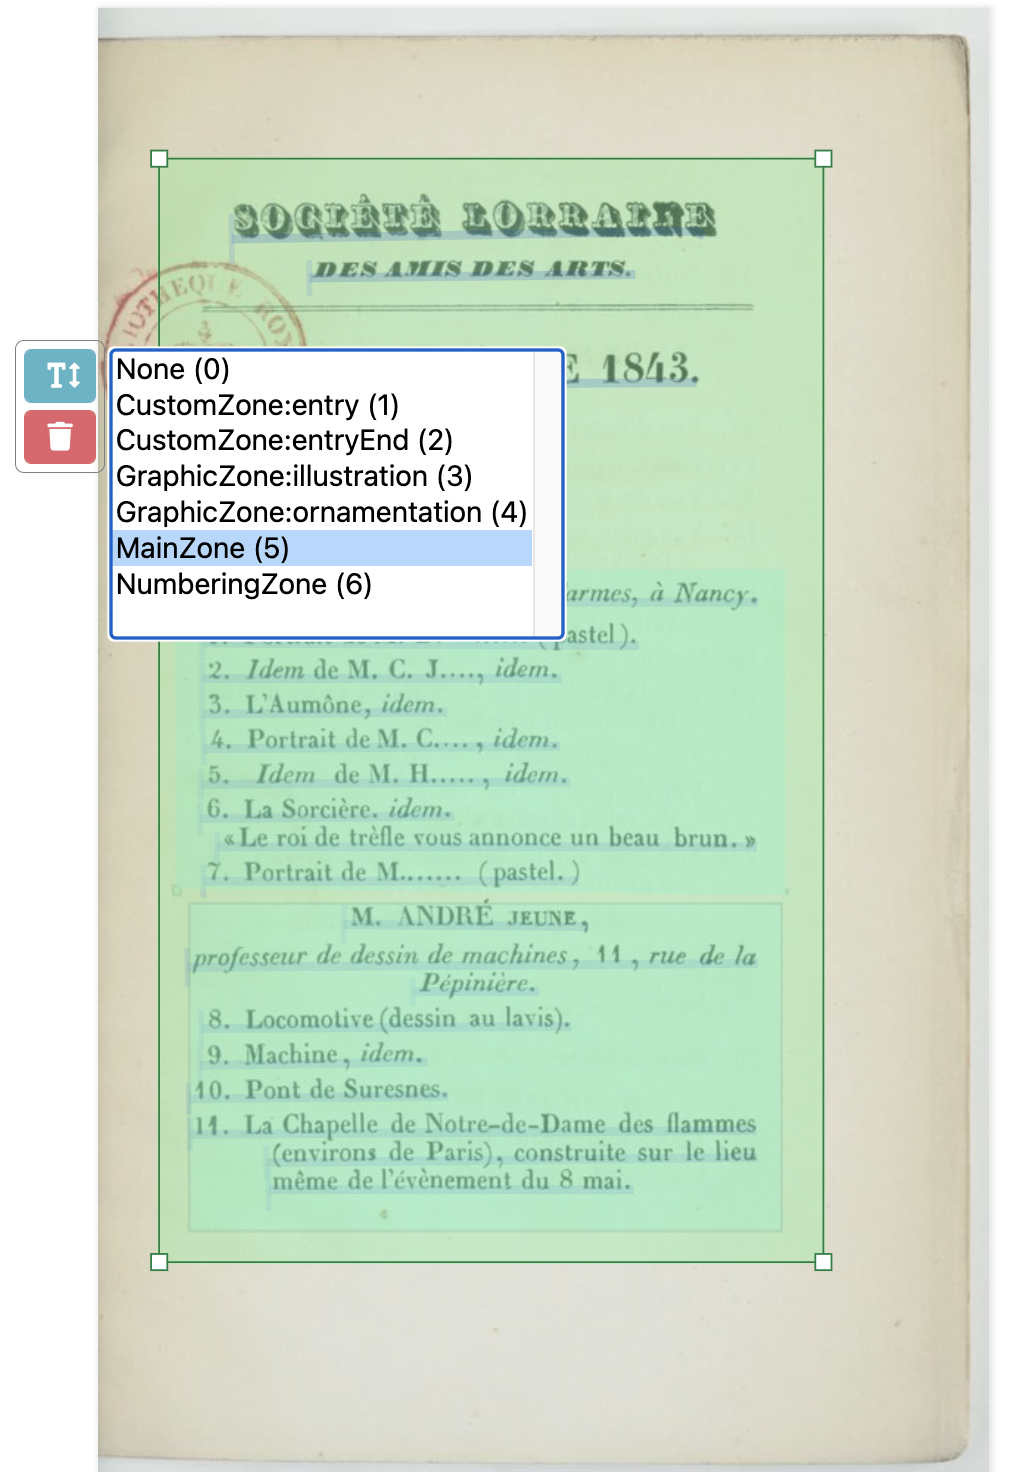
\includegraphics[scale=0.5]{MainZone_eScriptorium.png}		
	\caption{eScriptorium : MainZone}
\end{figure}

L'utilisateur doit segmenter manuellement toutes les pages du catalogue qui contienne des entrées. Il devra notamment veiller à ce qu'il n'y ai pas des conflits d'imbrication (des lignes qui dépassent leurs régions, des zones \texttt{CustomZone:Entry} qui dépassent la \texttt{MainZone}, etc.). Dans le cadre du catalogue Nancy 1843, nous allons segmenter une page sans entrées et cinq pages avec des entrées (pages 3-7) ; cela permettra de montrer comment le script traite une page qui ne contient pas d'entrées.


\section{Output ALTO}

À présent, l'utilisateur a transcrit et segmenté ses pages. Il faut maintenant récupérer le fichier ALTO en \texttt{output} d'eScriptorium afin de l'utilser comme \texttt{input} du script extractionCatalogs.

Pour récupérer ces fichiers, comme indiqué sur la figure \ref{frise2}, l'utilisateur doit [1] cliquer sur l'onglet "Images" pour retourner sur la frise des images, puis [2] cocher sur les images à télécharger et [3] cliquer sur "Export". Il doit veiller à respecter les indications de la figure \ref{modalites} : [1] le modèle de reconnaissance de caractères de l'export doit correspondre à celui qui a été utilisé, [2] les documents en \texttt{output} doivent être des fichiers ALTO, il doit [3] cocher sur "include images" et [4] vérifier que toutes les régions de l'ontologie soient cochées. [5] En cliquant sur "Export", un avertissement vert apparaît en haut à droite de la page si celui-ci est réussi, dans lequel il faut cliquer sur "Download" (figure \ref{download}).

\begin{figure}[ht]
	\centering
	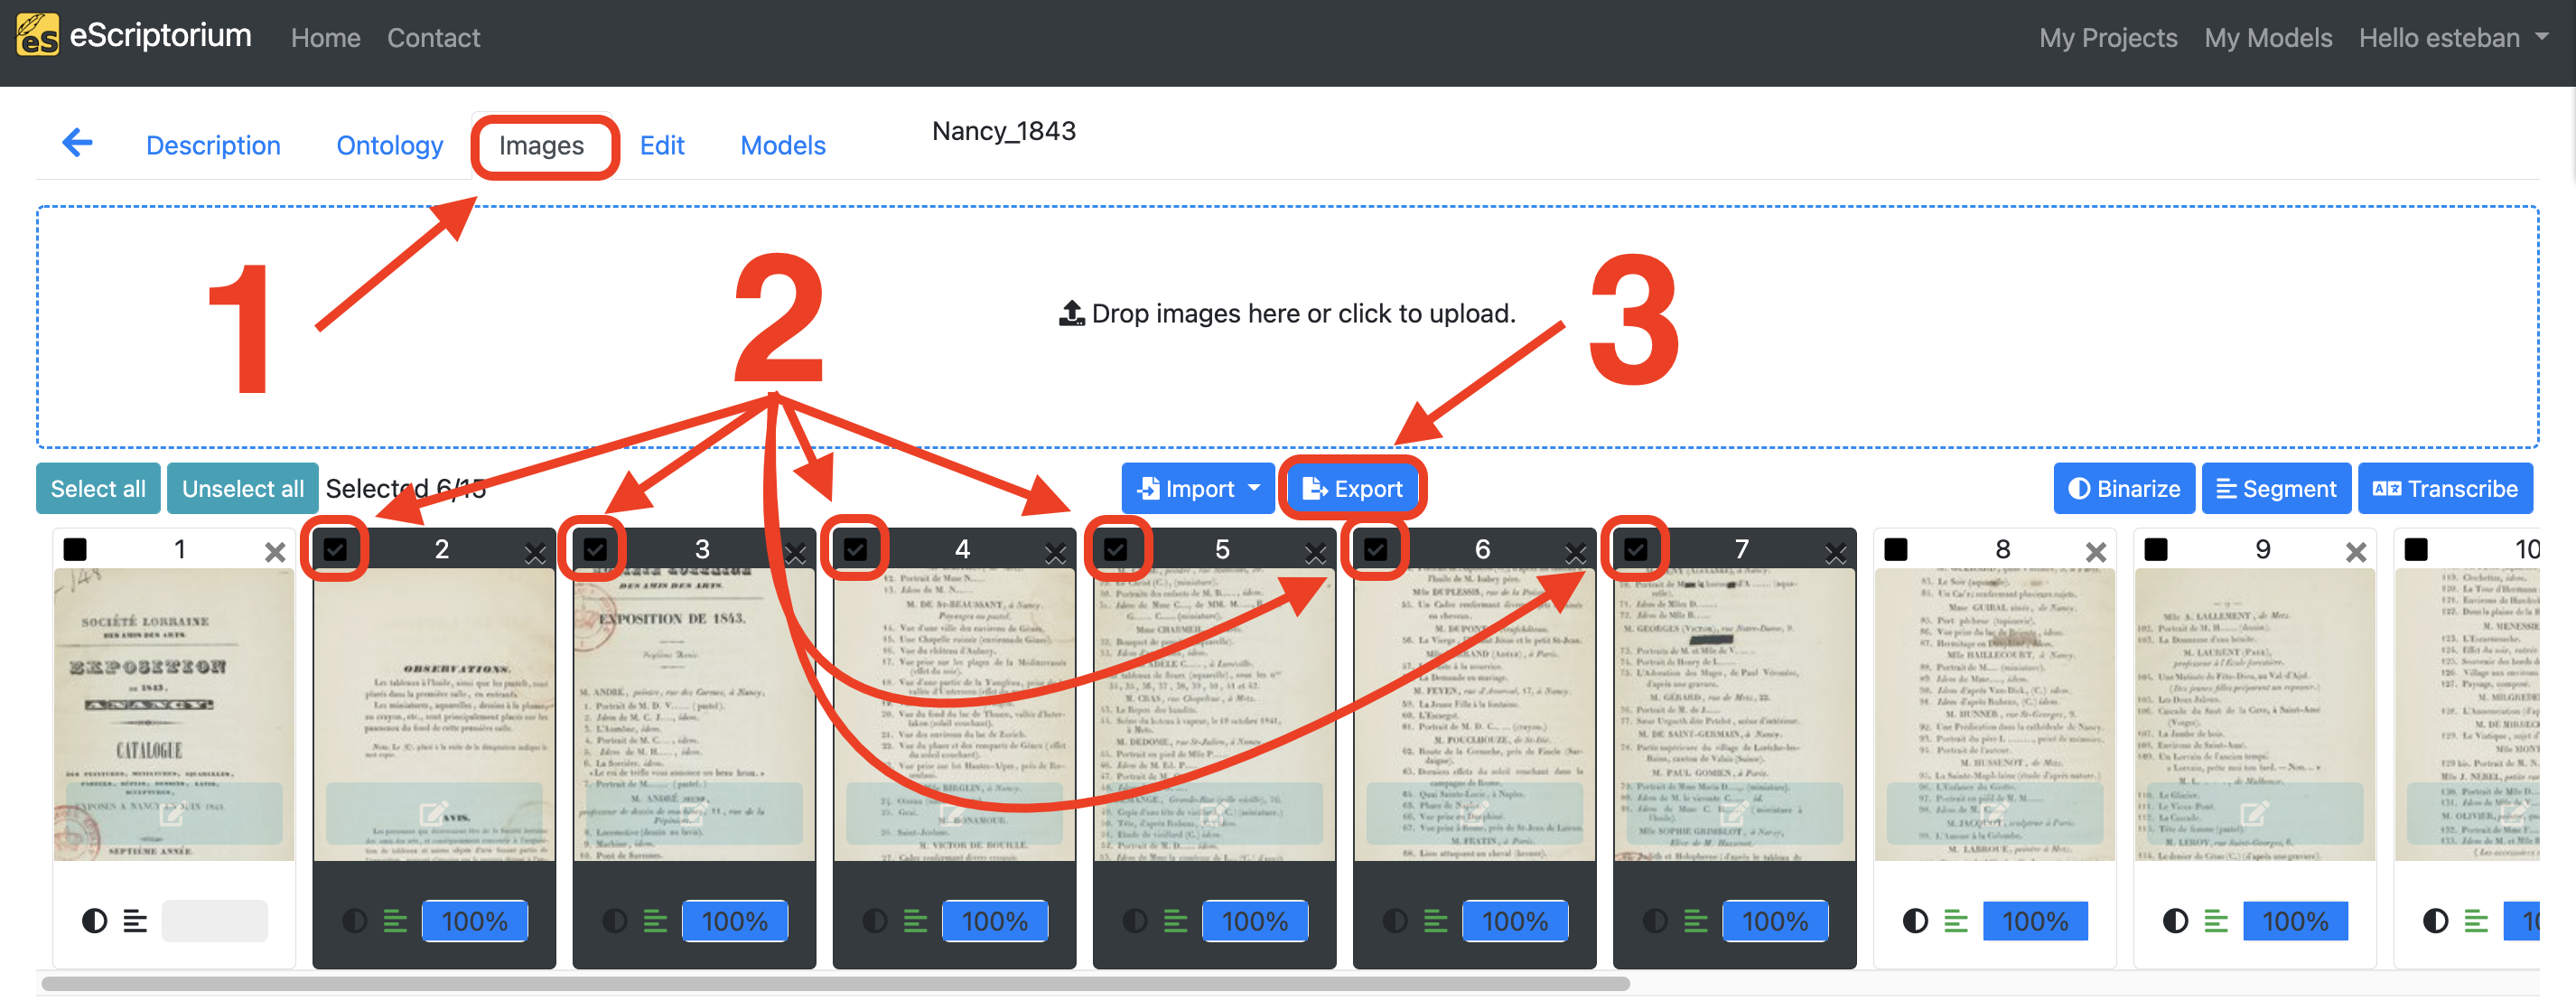
\includegraphics[scale=0.3]{export_eScriptorium.png}		
	\caption{eScriptorium : télécharger les fichiers ALTO}
	\label{frise2}
\end{figure}
\begin{figure}[ht]
	\centering
	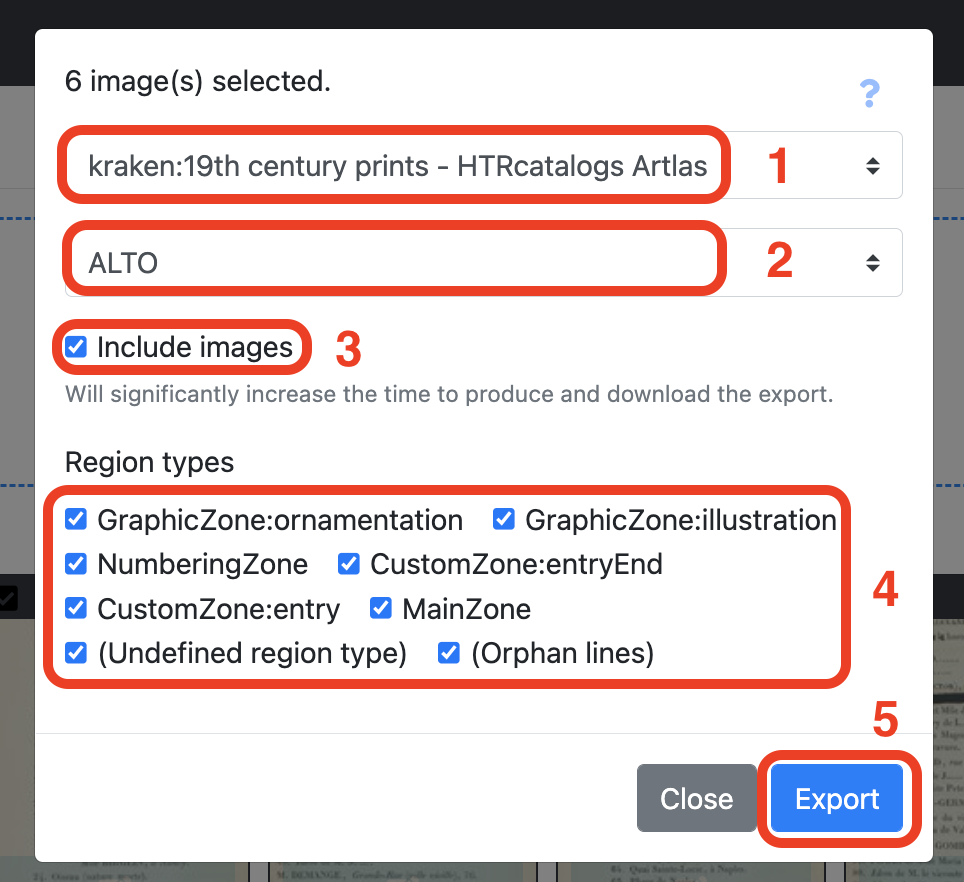
\includegraphics[scale=0.4]{export2_eScriptorium.png}		
	\caption{eScriptorium : modalités d'export}
	\label{modalites}
\end{figure}
\begin{figure}[ht]
	\centering
	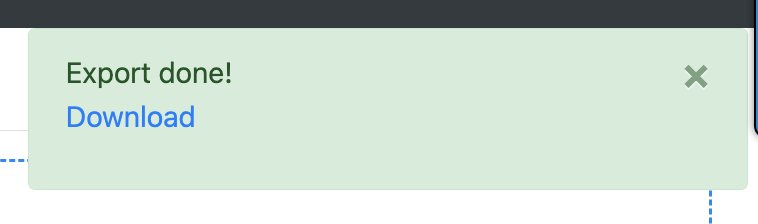
\includegraphics[scale=0.5]{download_eScriptorium.png}		
	\caption{eScriptorium : Download}
	\label{download}
\end{figure}

L'utilisateur télécharge ainsi un fichier \texttt{ZIP} qui contient les images du catalogue, et autant de fichiers ALTO4 contenant leurs transcriptions et leurs segmentations. Il peut être utile de rennomer les fichiers afin de les rendre plus compréhensibles à l'oeil humain, mais cela n'est pas obligatoire et implique de manipuler les fichiers ALTO. Cela n'est pas obligatoire, tant que les fichiers gardent un ordre numérique, mais il peut-être intéressant pour les étudiants de s'aventurer à faire des changements manuels sur ce type de fichier. Pour le catalogue Nancy 1843, on va suivre la convention de nommage suivante :
\begin{normalsize}
	\begin{minted}{bash}
Cat_Nancy_1843_typo_0000.jpg - Cat_Nancy_1843_typo_0005.jpg 
Cat_Nancy_1843_typo_0000.xml - Cat_Nancy_1843_typo_0005.xml
	\end{minted}
\end{normalsize}
Après avoir rennomé chaque fichier, il faut actualiser le nom de l'image à laquelle chaque fichier ALTO fait référence, afin que les deux fichiers restent liés. Notons pourtant qu'il s'agit uniquement d'exposer des bonnes pratiques, puisque cela ne va affecter en rien le programme extractionCatalogs. Pour le faire, il faut ouvrir chaque fichier ALTO et actualiser le nom de l'image (\texttt{.jpg}) à laquelle ce fichier fait référence dans la balise \texttt{<filename>} (voir la figure \ref{imageref})
\begin{figure}[ht]
	\centering
	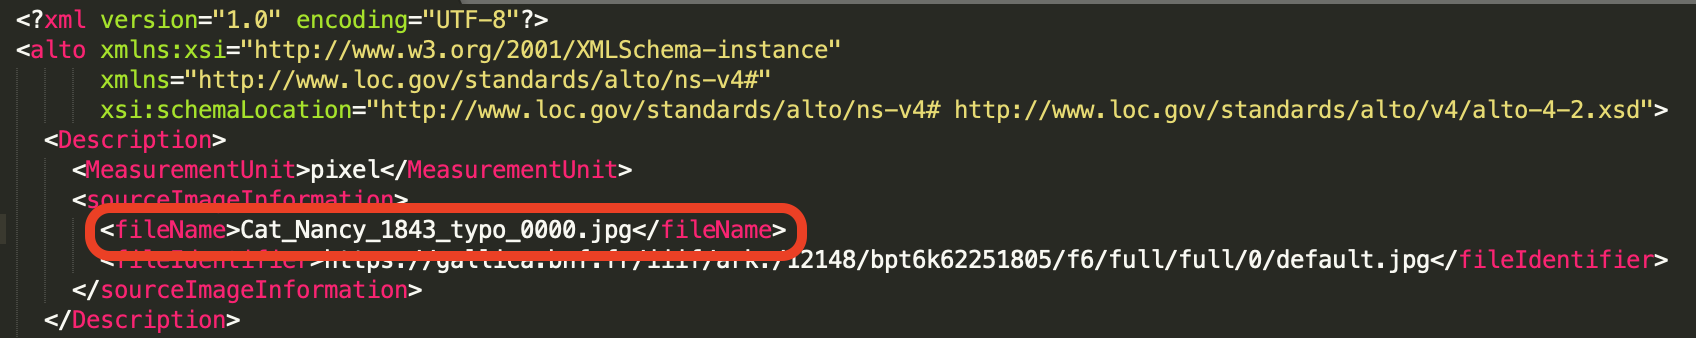
\includegraphics[scale=0.5]{filename.png}		
	\caption{ALTO : image liée}
	\label{imageref}
\end{figure}


ALTO\footcite{alto_editorial_board_alto_2004} (Analysed Layout and Text Object) est un standard XML permettant de rendre compte de la mise en page physique et de la structure logique d'un texte transcrit par reconnaissance optique de caractères (OCR). Si la transcription est correcte et que les zones de la page sont correctement saisies sur eScriptorium, le script extractionCatalogs sera extrêmement performant au moment de l'extraction et de la reconstruction des entrées du catalogue. 

La structure fondamentale d'un fichier ALTO est constituée par une balise racine \texttt{<alto>} contenant des sous-ensembles \texttt{<Description>}, \texttt{<Tags>} et \texttt{<Layout>} :

\begin{itemize}
	\item \texttt{<Description>} : métadonnées sur le fichier source. Le nom de l'image est indiqué, mais aussi le lien vers l'image iiif quand le fichier est issu d'un manifeste .
	\begin{figure}[ht]
		\centering
		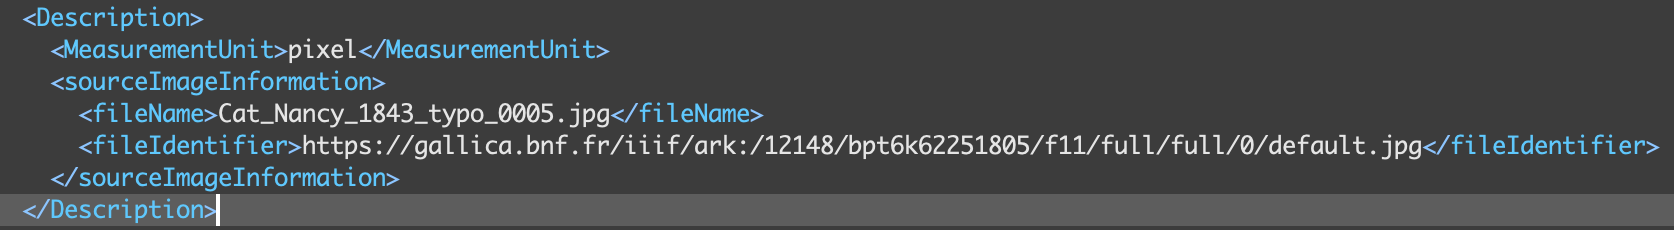
\includegraphics[scale=0.4]{description_alto.png}		
		\caption{ALTO : Description}
	\end{figure}

	\item \texttt{<Tags>} : établit des ID pour signaler les noms des régions (des tags). C'est ici que nous pourrons retrouver l'ontologie Segmonto. Ces ID seront utilisés dans la balise \texttt{<Layout>} pour signaler à quoi correspond chaque bloque de texte.
	\begin{figure}[ht]
		\centering
		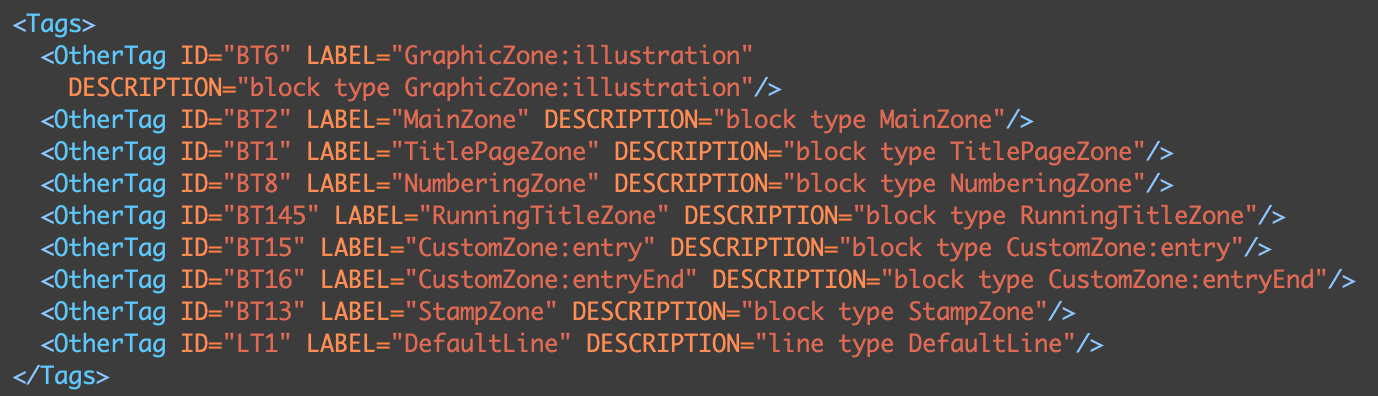
\includegraphics[scale=0.5]{tags_alto.png}		
		\caption{ALTO : Tags}
	\end{figure}
	
	\item \texttt{<Layout>} : Contient tout le texte transcrit. Nous retrouverons dedans des balises \texttt{<TextBlock>} : chacune correspond à une des régions signalées manuellement sur eScriptorium. Leur Attribut \texttt{TAGREFS} fait réfèrence à l'ID qui permet de connaître le nom de la zone dans la balise \texttt{<Tags>}. La balise \texttt{<Shape>} indique la position du \texttt{TextBLock} dans la page. Un \texttt{TextBlock} doit contenir des balises \texttt{<TextLine>}, qui elles mêmes contiennent des balises \texttt{<Shape>} et des balises \texttt{<String>}. C'est dans l'attribut \texttt{CONTENT} de cette dernière que se trouve le texte transcrit. Dans l'exemple de la figure \ref{alto4}, l'attribut \texttt{TAGREFS="BT15"} fait réfèrence au type de région \texttt{CustomZone:entry}.
	\begin{figure}[ht]
		\centering
		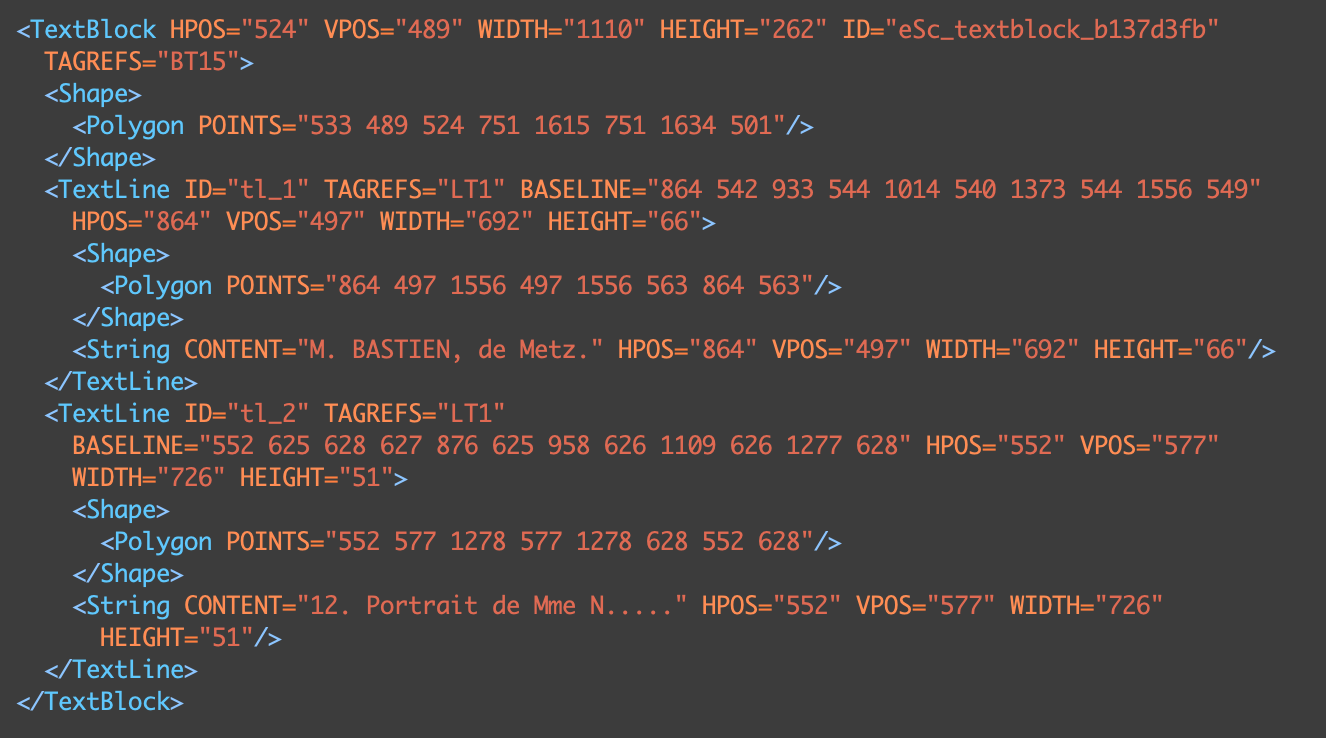
\includegraphics[scale=0.5]{textblock_alto.png}		
		\caption{ALTO : Layout}
		\label{alto4}
	\end{figure} 	
\end{itemize}

L'utilisateur peut corriger directement ces fichiers ALTO (pour préciser le découpage et les imbrications des régions, le contenu des lignes, les noms des zones), mais cela risque d'être très difficile pour un néophyte. Normalement, toutes les corrections (transcriptions et segmentations) sont faisables sur l'interface eScriptorium, ou bien sur le tableau produit par le programme extractionCatalogs (il est donc conseillé aux étudiants de corriger directement l'\texttt{output}). Cependant, il est possible et parfois souhaitable, dans un cadre pédagogique, de corriger les fichiers XML (ALTO, TEI) pour observer les conséquences que cela a sur le fonctionnement du script extractionCatalogs. 

Cette possibilité d'approfondissement des difficultés peut être intéressante pour aborder des groupes d'étudiants avec des décalages plus ou moins importants de culture numérique. Si l'utilisation de l'interface ou du guide sur le Notebook leur est trop facile, ils peuvent explorer les logiciels et technologies que ce dernier leur présente : iiif, fichiers ALTO, script python, fichier TEI produit (puisque celui-ci est utilisé pour produire le tableur CSV). 




\chapter{Utiliser le script python "extractionCatalogs"}

Une fois le travail de transcription automatique, de segmentation manuelle et de correction terminé, l'utilisateur téléchargera sur la plateforme eScriptorium un dossier contenant les images de son catalogue (elle seront toujours en format \texttt{.jpg}) et autant de fichiers XML ALTO contenant l'encodage du texte et des zones.

Le dossier peut être placé n'importe où en local ; il faudra indiquer le chemin au script extractionCatalogs. Ce chemin peut-être absolu (partir de la racine de l'ordinateur), ou bien relatif au dossier du script. Il peut-être est donc utile de créer un dossier à l'intérieur (ou proche) du dossier \texttt{extractionCatalogs}. Pour le catalogue Nancy 1843, nous avons créé un dossier \mintinline{bash}|exemples_guide| dans \mintinline{bash}|extractionCatalogs|. Ce dossier contient d'autres exemples qui sont évoqués aussi bien dans ce chapitre que dans le guide d'utilisation simplifié Jupyter Notebook. 

Le script extractionCatalogs va chercher et traiter les fichiers ALTO contenus dans le dossier indiqué. Il va utiliser les informations de segmentation pour pour reconstituer les entrées, ainsi que des expressions régulières pour analyser chaque ligne et déterminer si elle correspond à un exposant, à une œuvre ou à des informations complémentaires. Dans certains cas, il sera possible de déterminer la nature des informations complémentaires.

Le script est l'objet d'améliorations continues. En son état actuel, il est performant aussi bien pour ses visées pédagogiques que pour la production de données satisfaisantes. Il peut tout de même faire l'objet d'améliorations et d'évolutions, raison pour laquelle il est aussi important de le consulter directement pour comprendre en profondeur son fonctionnement. Dans le cadre du projet pédagogique du certificat en humanités numériques, mais aussi en prévision des stages à venir, une partie conséquente du développement du prototype établi par Juliette Janès en 2021 à consisté à améliorer son arborescence, à améliorer sémantiquement les noms des fonctions et des variables, à consolider les descriptions des fonctions, et à commenter profusément le code pour le rendre rapidement compréhensible. L'utilisateur peut donc ouvrir les fichier \texttt{.py} du dossier \texttt{extractionCatalogs}, qui contiennent tout le programme python. Il n'aura pas besoin d'intervenir dessus, et sera accompagné tout au long de sa lecture.

\section{Commandes du script}
La commande pour lancer le script a été simplifiée à l'extrême. Avant notre mission, il fallait faire une analyse préalable du catalogue pour indiquer au script, d'après une typologie, quelle était sa structure. Il n'était pas possible de choisir l'emplacement, et il fallait indiquer deux fois le nom du catalogue (une en tant qu'ID, un deuxième en tant que nom du fichier TEI). De plus, il y avait de nombreuses contraintes/erreurs techniques qui rendaient le lancement problématique. En l'état actuel, le script marche avec la totalité des catalogues du Corpus (37), contre 6 précédemment. En plus, le script est capable d'indiquer sur le terminal de manière claire pour un néophyte s'il y a des erreurs ou des problèmes qui l'empêchent de fonctionner.  

Voici le modèle de commande pour lancer le script : 

\begin{normalsize}
	\begin{minted}{bash}
!python3 run.py input output titre
	\end{minted}
\end{normalsize}

Pour traiter le catalogue Nancy 1843, nous devons construire la commande suivante :

\begin{scriptsize}
	\begin{minted}{bash}
!python3 run.py exemples_guide/Cat_Nancy_1843_page/ exemples_guide/extractions/ Nancy_1843
	\end{minted}
\end{scriptsize}

Voici ses composantes :

\begin{itemize}
\item \mintinline{bash}|!| indique à Jupyter Notebook que nous voulons lancer la commande sur le terminal. Si l'utilisateur lance la commande directement sur un terminal, il ne faut pas utiliser ce point d'exclamation

\item \mintinline{bash}|python3| indique que le script doit être exécute en langage python 3

\item \mintinline{bash}|run.py| est le fichier python que nous voulons exécuter. Tous les autres fichiers python se trouvent dans des sous-dossiers et sont appelés par celui-ci

\item \mintinline{python}|exemples_guide/Cat_Nancy_1843_page/| est le chemin vers les fichiers ALTO produits par eScriptorium. Ce dossier contient uniquement une page de catalogue (fichier \texttt{.jpg} + ALTO) afin que les premiers exemples restent simples

\item \mintinline{python}|exemples_guide/extractions/| est le chemin pour le dossier d'extraction que le script va produire. Si le chemin ou le dossier n'existent pas, le script les créé

\item \mintinline{bash}|Nancy_1843| est le nom souhaité pour le catalogue. Il sera utilisé pour le noms des fichiers en \texttt{output} (TEI et CSV) ainsi que pour les identifiants constitutifs des fichiers XML produits (TEI, restructurations ALTO) 
\end{itemize}

Le guide Jupyter Notebook permet de lancer et de visualiser les résultats de cette commande en exécutant la cellule avec le code correspondant  (COMMAND/ENTER, SHIFT/ENTER ou bouton "Run"). La cellule produit le message de terminal que l'on peut observer sur la figure \ref{commandelancee} : pour chaque page traitée, l'utilisateur obtient un récapitulatif concis et clair des étapes, ainsi qu'une visualisation structurée de l'extraction. Une fois toutes les pages traitées (l'exemple n'en contient qu'une), l'utilisateur obtient un résumé avec des statistiques générales du traitement de l'ensemble des pages. L'annexe C contient une versions en texte brut de cet output de terminal. 


\begin{figure}
	\centering
	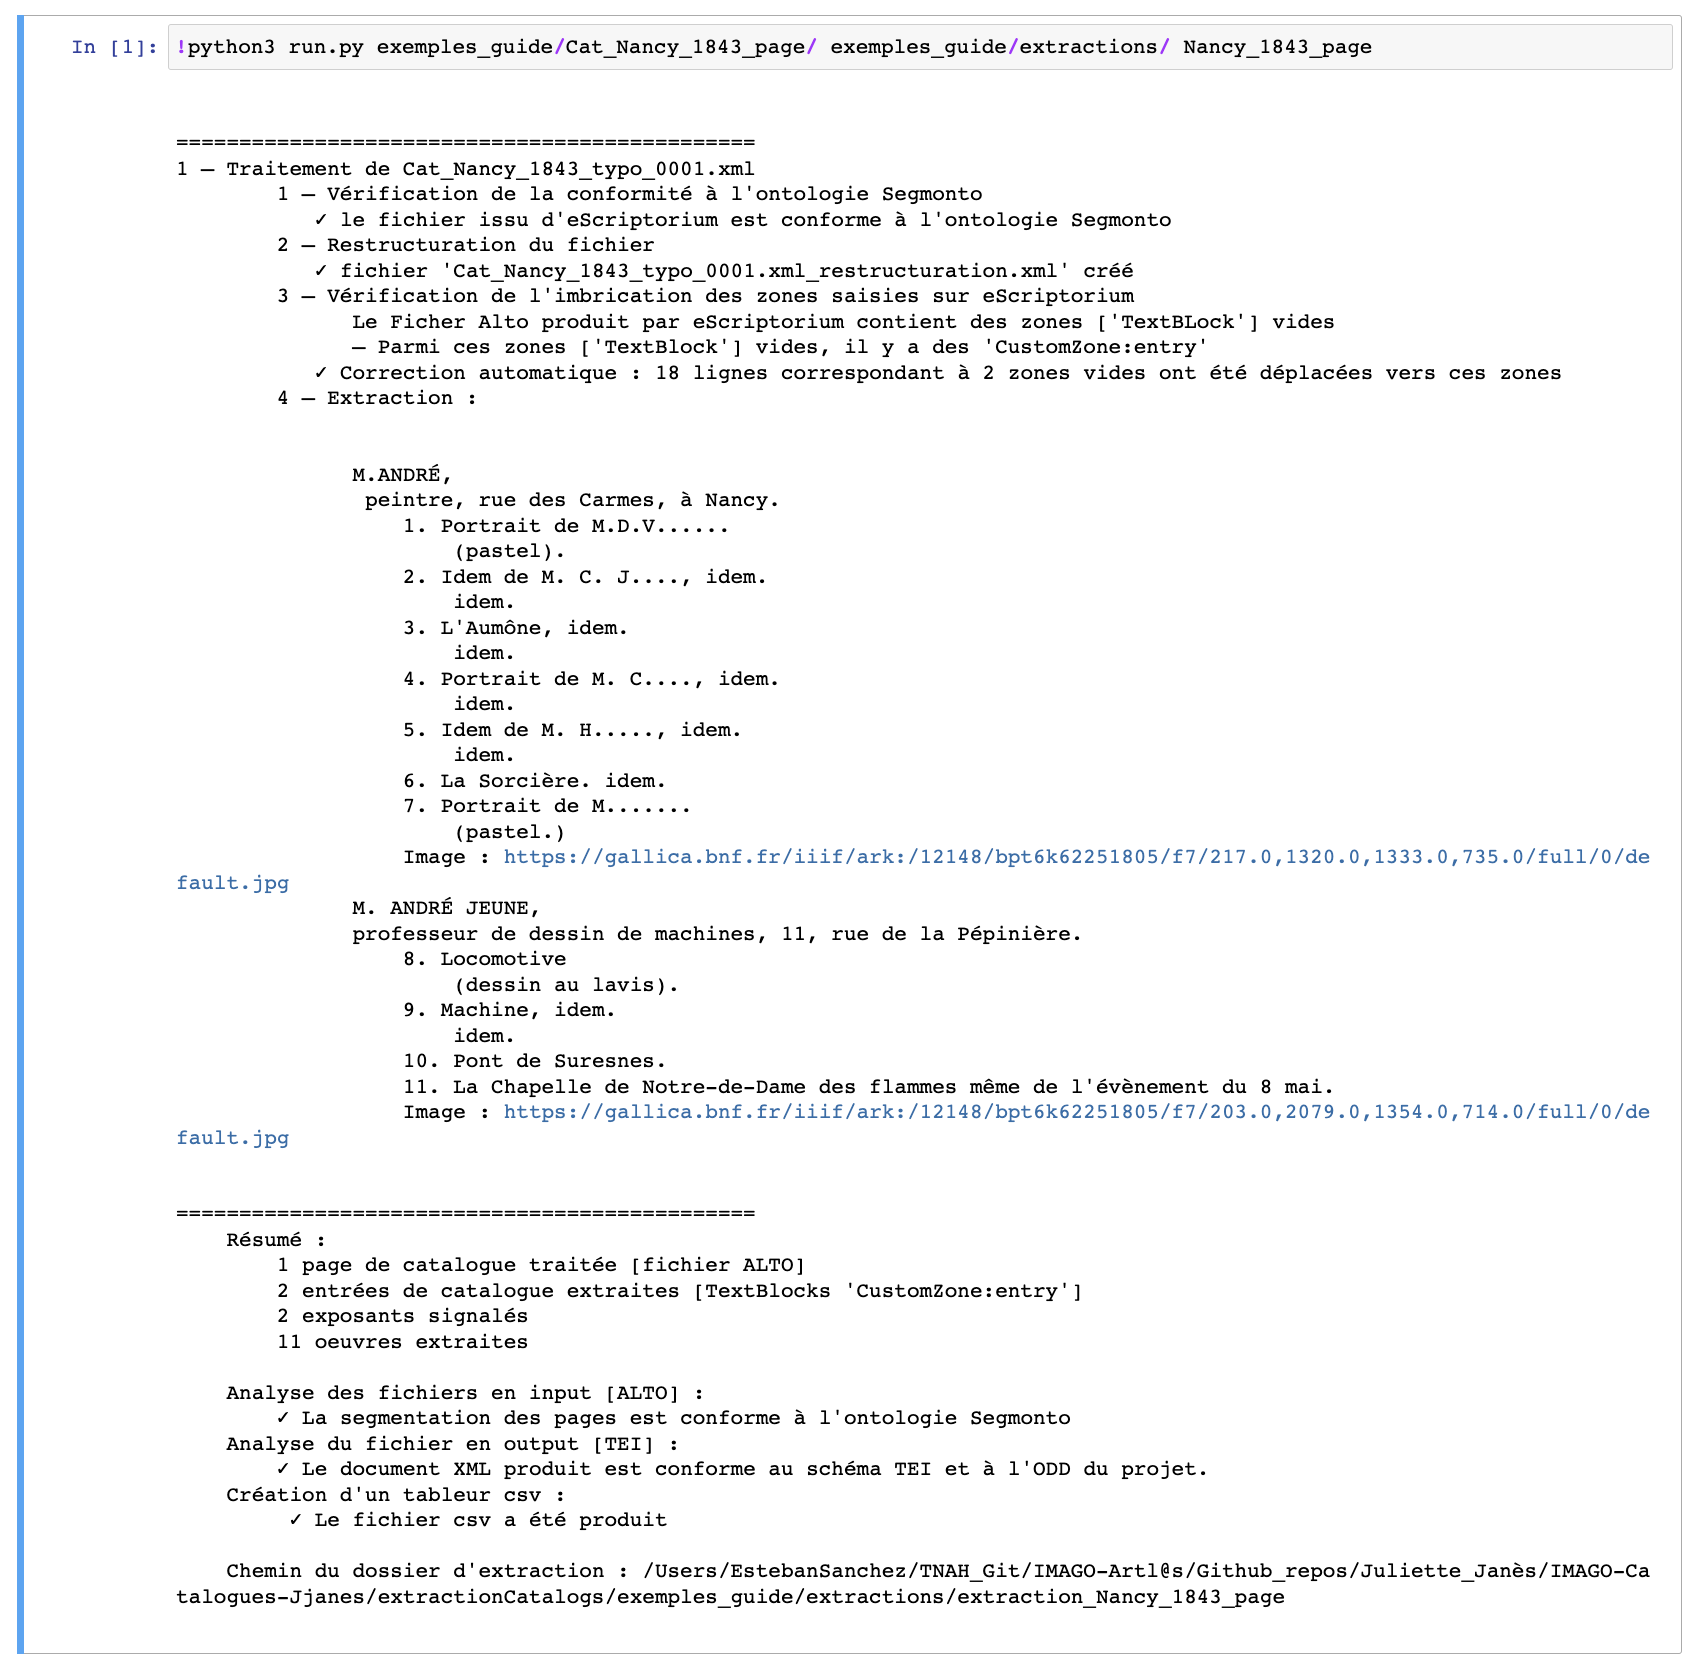
\includegraphics[scale=0.5]{jupyter_commande.png}
	\caption{Script : premier exemple d'extraction}	
	\label{commandelancee}
\end{figure}

La dernière information signale le chemin dans lequel l'extraction a été déposée. Dans le cas de l'exemple, il s'agit du dossier  \mintinline{bash}|extraction_Nancy_1843_page|. L'utilisateur peut consulter dedans les fichiers suivants :

\begin{itemize}
	\item \texttt{Nancy\_1843\_page.xml} : un fichier XML contenant la totalité des entrées extraites
	
	\item \texttt{CSV} : un dossier CSV avec deux tableurs :
	\begin{itemize}
		\item \texttt{Nancy\_1843\_page\_tableau\_simple.csv} : tableur simplifié pour lecture humaine
		\item \texttt{Nancy\_1843\_page\_tableau.csv} \_ tableur complet et utilisabe comme \texttt{input} pour la base de données Artl@s
	\end{itemize}

	\item \texttt{restructuration ALTO} : un dossier avec des fichiers ALTO "restructurés"  "resegmentés" : ils résultent d'une correction automatique des erreurs de saisie sur eScriptorium

	\item eventuellement, un fichier \texttt{.txt} indiquant des problèmes d'extraction (dans le cas de l'exemple, aucune erreur n'a été détectée)
\end{itemize}




\section{Fonctionnement du script}

Le guide Jupyter Notebook accompagne l'utilisateur dans le développement d'une culture numérique suffisante pour comprendre dans son ensemble l'\texttt{output} du script (messages de terminal, fichiers produits). Il lui permet aussi de comprendre la structure fondamentale du dossier contenant le script, ainsi que le code contenu. En fonction de ses besoins, il pourra consulter les fichiers pour accéder à des détails beaucoup plus approfondis, les script étant accompagné d'explications profuses et simples.

En tout état de cause, le Notebook, le script et de manière plus générale l'ensemble du pipeline ont été conçus pour qu'un utilisateur sans connaissances informatiques particulières puisse les utiliser, sans intervenir dans leur mécanique interne. Il suffit qu'il développe les capacités nécessaires (pour cela, il est accompagné par le Notebook et par ses enseignants) pour l'exécuter et pour pouvoir comprendre les messages et fichiers en \texttt{output}.

Cette section décrit le fonctionnament du script à travers des étapes fondamentales exécutées par le fichier \texttt{run.py}. Le dossier \texttt{extractionCatalogs} contient :

\begin{itemize}
\item \texttt{run.py} : fichier python principal qui exécute tous les fichiers \texttt{.py} secondaires, contenus dans les sous-dossiers \texttt{extractionCatalogs/extractionCatalogs/fonctions} et \texttt{extractionCatalogs/extractionCatalogs/variables}

\item \texttt{README.md} : fichier expliquant comment installer le script (ce sont les mêmes instructions que dans la partie \texttt{0.Introduction} du guide Notebook. Ces instructions sont expliquées de manière plus approfondie dans le chapitre 7 du mémoire)

\item \texttt{requirements.txt} : fichier \texttt{.txt} indiquant les paquets python externes dont le script à besoin pour fonctionner. Ces paquets sont installés lors de l'étape d'installation avec la commande \texttt{!pip install -r requirements.txt})

\item dossiers \texttt{exemples} : dossiers contenant des catalogues à l'état d'encodage ALTO ou d'extraction python :
\begin{itemize}
	\item \texttt{exemples\_guide} : exemple utilisés dans le guide Jupyter Notebook
	\item \texttt{exemples\_input} : totalité des catalogues du corpus Artl@s encodés en fichiers ALTO (sortie eScriptorium). Ils sont issus du travail collaboratif des stagiaires, étudiants et chercheurs contribuant au projet Artl@s. Le dossier contient pour l'instant des encodages relatifs à 37 catalogues d'exposition d'art du XIXe et XXe siècles.
	\item \texttt{exemples\_output} : extractions python pour chaque catalogue du corpus avec le script développé pendant le stage 2022. Ces dossiers permettent de constater les atouts et les limites actuelles du script qui fonctionne globalement de manière très satisfaisante. Quand il y a des soucis d'extraction, le script est systématiquement capable d'expliciter les problèmes.
\end{itemize}

\item \texttt{Guide – extraction de catalogues.ipynb} : guide Jupyter Notebook

\item dossier \texttt{env} : environnement virtuel contenant les paquets python. Ce dossier n'existe que dans les cas ou le script a été téléchargé hors de Google Colab (normalement, cela aura lieu sur Github)
\end{itemize}


\texttt{run.py} est le fichier exécuté par la commande \texttt{!python3 run.py}, suivie des indications secondaires (\texttt{input}, \texttt{output}, \texttt{nom du catalogue}). Ce fichier est la colonne vertébrale du script, puisqu'il contient tout le processus du début à la fin. Il appelle les autres fichiers \texttt{.py}, qui fonctionnent comme des extensions séparées pour que le script garde une structure logique et compréhensible par un être humain sous la forme d'une arborescence de dossiers. Ces autres fichiers \texttt{.py} sont des fonctions spécialisées, souvent longues, qui ont été rangées dans des sous-dossiers. Le fichier \texttt{run.py} exécute les opérations indiquées dans la liste qui suit. La même numérotation est utilisée dans les commentaires du fichier : il est donc possible de suivre la liste suivante et de parcourir le script en même temps.\\


\begin{itemize}

\item [1.1] On appelle les paquets externes, modules et fonctions nécessaires : nous allons faire appel, dossier par dossier et fichier par fichier, aux fonctions créés pour ce script et situées en dehors de \texttt{run.py} :
\begin{scriptsize}
	\begin{minted}{python}
from extractionCatalogs.fonctions.extractionCatEntrees import extInfo_Cat
from extractionCatalogs.fonctions.creationTEI import creation_header
from extractionCatalogs.fonctions.restructuration import restructuration_automatique #[...]
from extractionCatalogs.fonctions.Validations_xml import conformite_Segmonto, association_xml_rng
from extractionCatalogs.fonctions.XMLtoCSV import XML_to_CSV, csv_immediat
from extractionCatalogs.fonctions.automatisation_kraken.kraken_automatic import transcription
from extractionCatalogs.variables import contenu_TEI
from extractionCatalogs.fonctions.extractionCatEntrees_fonctions import ordonner_altos #[...]
	\end{minted}
\end{scriptsize}
Ces modules sont extraits des fichiers suivants :
\begin{itemize}
	\item \texttt{extractionCatEntrees.py}
	\item \texttt{creationTEI.py}
	\item \texttt{restructuration.py}
	\item \texttt{Validations\_xml.py}
	\item \texttt{XMLtoCSV.py}
	\item \texttt{variables.py}
	\item \texttt{extractionCatEntrees\_fonctions}
\end{itemize}

Nous allons aussi appeler des paquets externes au script. Certains d'entre eux ont été installés avec le fichier \texttt{requirements.txt}, d'autres sont intégrés à python3 et peuvent être appelés sans installation préalable. Pour notre script, nous avons besoin des paquets python suivants :
\begin{itemize}
	\item \texttt{lxml} : implémentation xml pour python, qui nous permettra de créér et de manipuler de objets xml
	\item \texttt{click} : permet de créér les commandes pour exécuter le script (\texttt{input}, \texttt{output}, \texttt{titre})
	\item \texttt{re} : implémentation regex pour python, qui nous permettra de construire et utiliser des expressions régulières
	\item \texttt{os} : permet de manipuler avec python des fichiers et dossiers présents sur l'ordinateur
\end{itemize}

\item [1.2] Création des commandes pour lancer le script sur le Terminal : le paquet \texttt{click} permet d'établir une communication avec le terminal, afin de demander en \texttt{input} des variables spécifiques. Dans notre cas, outre les commandes fondamentales \texttt{!python3 run.py}, nous utilisons \texttt{click} pour créer et demander d'autres éléments en \texttt{input} : \texttt{directory}, \texttt{output} et \texttt{titlecat}. Ce sont des chaînes de caractère que le script va parser pour en vérifier la validité et pour les utiliser en tant que variables.

\item [1.3] Création de la fonction principale du script : nous définissons la fonction \mintinline{python}|extraction()| qui constitue la totalité du script, puisqu'elle appelle toutes les fonctions secondaires et qu'elle produit les documents en sortie (TEI, CSV, restructurations ALTO et fichier \texttt{problèmes.txt}) :


\begin{normalsize}
	\begin{minted}{python}
def extraction(directory, output, titlecat, segmentationtranscription)
	# contenu de la fonction (+500 lignes)
	\end{minted}
\end{normalsize}

Tout ce qui suit est contenu dans cette fonction.\\

\item [2.1] Création d'un dossier pour les \texttt{output} : nous utilisons le paquet \texttt{os} pour traiter les chemins indiqués (\texttt{input} et \texttt{output}), et pour créer les chemins qui seront nécessaires au script pour aller chercher puis produire les fichiers.

\item [2.2] Création immédiate d'un fichier CSV, si la chaine "csv" est contenue dans le titre du catalogue (variable \texttt{titlecat} passée avec la commande) : lorsque le titre du catalogue indiqué dans la commande se termine par \texttt{.csv}, le script va tout simplement produire un tableur avec les fichiers qui existent déjà, sans traiter les fichiers ALTO en input ni créer de fichier TEI. Cela est utile lorsqu'on a déjà exécuté préalablement le script, que nous avons fait des modifications manuelles sur le fichier TEI, et que nous voulons simplement actualiser notre tableur CSV. Dans ce cas, le script s'arrêtera immédiatement à cette étape.

\item [2.3] création du fichier \texttt{problèmes.txt} et traitement de l'option \texttt{-st} : on vérifie les chemins existants pour créér (ou remplacer) le fichier \texttt{problèmes.txt}. Nous traitons aussi une commande en option, \texttt{-st}, qui permet de demander une transcription automatique au logiciel kraken. Dans ce cas, l'input devra être constitué uniquement d'images. Cette option, développée lors du stage 2021, ne fonctionne pas pour plusieurs raisons : les commandes kraken indiquées ne sont plus d'actualité, la segmentation automatique donne des résultats très défaillants, et la transcription automatique ne peut pas être corrigée. L'option \texttt{-st} reste donc une implémentation expérimentale, en prospective d'avancements techniques hypothétiques qui permettraient de faire des transcriptions/segmentations automatiques suffisamment performantes comme pour ne plus avoir à utiliser eScriptorium. Dans ce cas, le script fonctionnerait de manière autonome et constituerait la totalité du pipeline. Il serait alors intéressant de pouvoir passer en commande directement un lien iiif comme ensemble d'images à traiter.\\

\item [3] Création d'un arbre TEI : nous utilisons le paquet \texttt{lxml} pour construire un arbre TEI conforme au projet (lequel qui possède un schéma et une ODD spécifiques développés lors du stage 2020)\footcite{corbieres_du_2020}. Le script crée, un par un, les sous-éléments des l'arbre (\texttt{tei}, \texttt{teiHeader}, \texttt{text}, \texttt{body}, \texttt{list}, etc.). Pour créér le \texttt{teiHeader}, le script utilise le gabarit suivant : 
\begin{normalsize}
	\begin{minted}{python}
variables/gabarit_teiHeader_IMAGO.py
	\end{minted}
\end{normalsize}
Ce document est adapté au projet Artl@s et permet que les métadonnées de l'encodage soient complètes et facilement modifiables à travers de variables. Cela facilite les modifications, puisqu'il n'est plus nécessaire d'intervenir sur la fonction de construction de l'arborescence TEI. Il est possible de construire d'autres gabarits adaptés à d'autres projets, grâce au document suivant :
\begin{normalsize}
	\begin{minted}{python}
variables/gabarit\_teiHeader\_vide.py
	\end{minted}
\end{normalsize}
Il faut remplir dedans les noms des variables selon les besoins du projet, et en indiquant le nom de ce document sur le fichier \mintinline{bash}|variables/contenu_tei.py| :
\begin{figure}[ht]
	\centering
	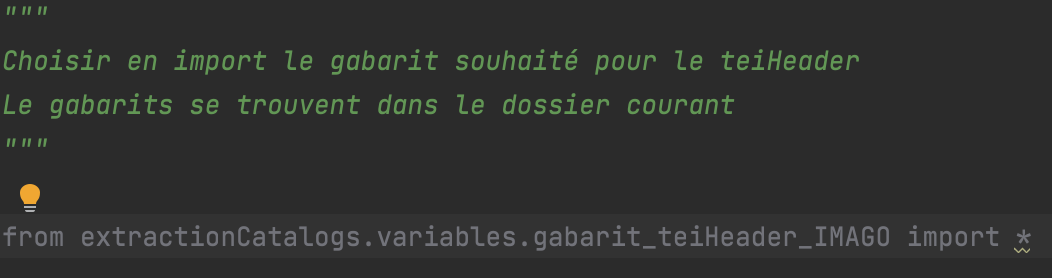
\includegraphics[scale=0.5]{gabarit.png}		
	\caption{Script : gabarit personnalisé pour le teiHeader}
\end{figure}

Cette fonctionnalité à déjà été utilisée par une étudiante du certificat en humanités numériques de l'Unige, Frédérine Pradier, dont on a intégré au dossier le gabarit : 
\begin{normalsize}
	\begin{minted}{python}
variables/gabarit\_teiHeader\_PictoCatalogs.py
	\end{minted}
\end{normalsize}

\item [4.1] Traitement préalable des ALTO en input : nous allons maintenant aller chercher les fichier ALTO contenus dans le dossier signalé par la commande. Nous allons faire une boucle afin que chaque fichier suive le même traitement, un par un.
\begin{normalsize}
	\begin{minted}{python}
for fichier in liste_en_ordre:
	# contenu de la fonction (+100 lignes)
	\end{minted}
\end{normalsize}
\item [4.2] On analyse la conformité et la structure des fichiers ALTO : une fonction secondaire permet de vérifier si les zones nommées correspondent à l'ontologie Segmonto. Les erreurs éventuelles seront signalées dans le fichier \texttt{problèmes.txt}

\item [4.3] Restructuration des ALTO en input : une première restructuration a lieu. Parfois, les fichiers ALTO produits par eScriptorium présentent les éléments \texttt{TextBlock} (qui correspondent à des entrées de catalogue) de manière désordonnée. Il s'agit de les mettre dans le bon ordre avec la feuille de transformation XSL \mintinline{bash}|Restructuration_alto.xsl|. Un dossier \texttt{restructuration ALTO} est créé et les fichiers restructurés y sont déposés.

\item [4.4] Restructuration eventuelle de la segmentation des ALTO en input ("resegmentation" est le mot utilisé dans le nom des fichiers pour différencier cette deuxième restructuration) : il existe un autre problème, beaucoup plus complexe, dans les fichiers ALTO produits par eScriptorium. Selon l'ordre de saisie des lignes et des régions sur l'interface, le fichier ALTO produit peut avoir des structures très variables : des fois, les \texttt{TextBlock} qui contiennent le texte transcrit ne correspondent pas à des \texttt{Custom:entry} (comme attendu), mais à des \texttt{MainZone}, ce qui rend le fichier intraitable par le script. D'autres erreurs dans ce registre peuvent avoir lieu. Nous avons donc créé une fonction qui utilise les informations de positionnement spatial de chaque \texttt{TextBlock} pour corriger toutes les erreurs d'imbrication du fichier. Si des erreurs sont détectées, la fonction les corrige dans des fichiers "\texttt{resegmentation}" qui vont être déposés à coté des fichiers "\texttt{restructuration}". Cette fonction à l'intérêt de corriger un problème inhérent à l'interface eScriptorium en calculant les régions selon les informations du fichier ALTO. Elle peut donc être reprise dans le cas d'autres projets pour adapter les imbrications de l'\texttt{output} selon les besoins. Cette fonction a permis de passer de 6 catalogues traitables à 37 dans le corpus Artl@s d'encodages en ALTO.\\

\end{itemize}
\begin{scriptsize}
	\begin{minted}{python}
for TextBlock in TextBlocks_vides:
	# on récupère l'ID du TextBlock courant, et on l'utilise pour construire le chemin xpath vers les
	# attributs qui signalent sa position dans la page :
	TextBlock_ID = TextBlock.xpath("@ID", namespaces=NS)[0]
	# on utilise float et non pas int pour convertir les chiffres car les données peuvent contenir des décimales :
	HPOS_T = float(Alto.xpath("//alto:TextBlock[@ID='{}']/{}".format(TextBlock_ID, "@HPOS"), namespaces=NS)[0])
	VPOS_T = float(Alto.xpath("//alto:TextBlock[@ID='{}']/{}".format(TextBlock_ID, "@VPOS"), namespaces=NS)[0])
	WIDTH_T = float(Alto.xpath("//alto:TextBlock[@ID='{}']/{}".format(TextBlock_ID, "@WIDTH"), namespaces=NS)[0])
	HEIGHT_T = float(Alto.xpath("//alto:TextBlock[@ID='{}']/{}".format(TextBlock_ID, "@HEIGHT"), namespaces=NS)[0])

	# On calcule quelles TextLignes sont associées à quels TextBLocks vides
	# ATTENTION : si les régions n'ont pas été saisies correctement sur escriptorium, cette fonction est susceptible
	# de ne pas marcher.  Ceci arrive par exemple quand quelqu'un dessine 
	# une ligne qui dépasse le TextBlock qui est censé le contenir. Cette 
	# situation s'avérant assez courante, nous avons développé une manière 
	# de la contourner presque systématiquement em ajoutant une marge
	# d'erreur dans le calcul
	
	# on appelle le dictionnaire de zones des lignes et on boucle sur chaque ligne :
	for ligne_ID in dic_zones_lignes:
		# on créé des variables signalant les zones de la ligne courante :
		HPOS_L = float(dic_zones_lignes[ligne_ID]["HPOS_L"])
		VPOS_L = float(dic_zones_lignes[ligne_ID]["VPOS_L"])
		WIDTH_L = float(dic_zones_lignes[ligne_ID]["WIDTH_L"])
		HEIGHT_L = float(dic_zones_lignes[ligne_ID]["HEIGHT_L"])
		# On fait les calcules permettant de déterminer si une TextLine est
		# contenue par un TextBlock dans la page :
		# Pour les comprendre, la documentation visuelle des régions iiif peut être utile :
		# https://iiif.io/api/image/2.1/#image-request-parameters
		if HPOS_T <= HPOS_L + 50:
			if VPOS_T <= VPOS_L + 50:
				if HPOS_T + WIDTH_T + 50 >= HPOS_L + WIDTH_L:
					if VPOS_T + HEIGHT_T + 50 >= VPOS_L + HEIGHT_L:
						# variable signalant la ligne courante :
						contenu = Alto.xpath("//alto:TextLine[@ID='{}']".format(ligne_ID), 
							namespaces=NS)[0]
						# on l'ajoute au TextBlock courant :
						TextBlock.append(contenu)
	\end{minted}
\end{scriptsize}

\begin{itemize}
\item [5.1] Extraction des entrées : Maintenant que nous nous sommes assurés que les fichiers ALTO sont correctement structurés, nous pouvons extraire leurs informations et reconstituer les entrées du catalogue. Le script fait appel à une série de fonctions qui traitent chaque ligne, de chaque entrée, de chaque page. Ces fonctions vont utiliser des expressions régulières complexes pour déterminer si la ligne courante est le nom-prénom d'un auteur, une œuvre, ou bien une information complémentaire (adresse, biographie, etc.). Si le travail de correction des transcriptions automatiques et la segmentation manuelles sont correctes, ces fonctions produiront des résultats très satisfaisants. 
\item [5.2] Après avoir reconstitué chaque entrée de catalogue, ces fonctions les adaptent à l'arbre TEI et l'intègrent dedans. Elles permettent aussi de détecter plusieurs problemes d'extraction, qui seront indiqués dans le fichier \texttt{problemes.txt} afin que l'utilisateur/utilisatrice puisse les corriger facilement (de manière générale, il s'agit de lignes qui n'ont pas été reconnues et qui ont été exclues de l'arbre TEI).\\	

\item [6] \texttt{output} : TEI et CSV : nous arrivons aux dernières étapes du script. L'arbre TEI est prêt, on va l'écrire dans un fichier déposé dans le chemin \texttt{output} indiqué dans la commande. Selon les erreurs de transcription, de segmentation, ou de reconnaissance, ce fichier comportera des erreurs. Il sera utilisé par le script pour produire deux tableurs CSV, déposés dans un dossier \texttt{CSV}. Selon les erreurs contenues dans le fichier TEI, ces fichiers CSV comporteront des erreurs. Le premier est une version simplifiée adaptée à la lecture humaine et utile pour les corrections manuelles. Le deuxième comporte de nombreuses colonnes et constitue un gabarit pouvant alimenter la base de donnée BasArt du projet ARTl@S.\\

\item [7] Informations à afficher sur le terminal : Finalement, le script construit et affiche des messages d'information ou d'erreur, lesquels ont été produits tout au long du script. Ces messages permettent que l'utilisateur/utilsiatrice puisse évaluer simplement le résultat du pipeline. Ils signalent comment corriger les éventuelles erreurs, et affichent des résumés des processus réussis. C'est à travers de cet \texttt{output} que l'utilisateur/utilisatrice est susceptible de prendre en main efficacement le programme : il s'agit de produire des explications, même dans les cas ou le traitement des fichiers ne soit pas satisfaisant.
\end{itemize}



\section{Expressions régulières}

L'utilisation d'expressions régulières (regex) pour reconnaître les lignes du catalogue est une étape fondamentale du script. Celles-ci sont implémentées grâce au pacquet externe python \texttt{re}. Le programme extractionCatalogs est doté de regex adaptées à la très grande majorité des cas possibles, mais il pourrait arriver que l'utilisateur soit mené à devoir les adapter à son catalogue. L'implémentation regex résulte d'un choix pragmatique qui, pour ce cas spécifique, a donné la priorité à l'efficacité face à la pédagogie. Le souhait initial de Béatrice Joyeux-Prunel était que l'interface Jupyter permette que les étudiants indiquent des regex simples adaptées à leurs catalogues. Cependant, ce type de manipulation implique que le script ne soit pas immédiatement fonctionnel, et face à la variété des cas possibles, qui est ample mais semble limitée par la répétition de cas usuels, il a finalement paru préférable de développer des regex longues et solides. Elles s'avèrent difficiles à expliquer à des étudiants, mais pour l'instant très satisfaisantes sur le plan technique. Par ailleurs, les regex étant rassemblées dans un même document \texttt{instantiation\_regex.py}, il est finalement très simple d'adapter les variables à des cas spécifiques avec des regex courtes personnalisées. 

Les catalogues des expositions d'art du XIXe et XXe siècle comportent une grande variété de formats de présentation des exposants et de leurs oeuvres. Il est possible de dire que chaque catalogue est une configuration unique de conventions qui elles peuvent se répéter souvent. La figure \ref{entrees} présente quelques exemples. Ceux-ci sont inclus dans l'annexe B, qui présente des échantillons de tous les catalogues du corpus Artl@s. Notons qu'on peut ainsi aussi observer des découpes correctes des zones Segmonto \texttt{CustomZone:entry}. 

\begin{figure}[ht]
	\begin{subfigure}{0.5\textwidth}
		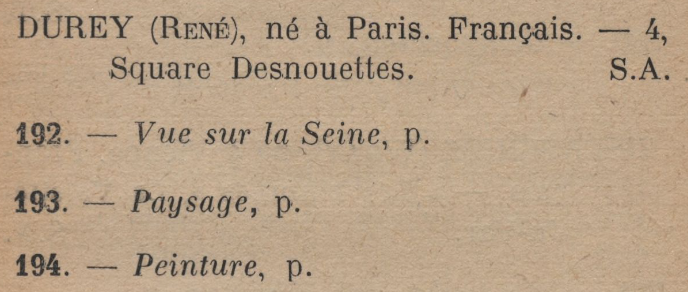
\includegraphics[scale=0.5]{automne1940.png} 
		\centering
		\caption{Salon d'automne 1940}
	\end{subfigure}
	\begin{subfigure}{0.5\textwidth}
		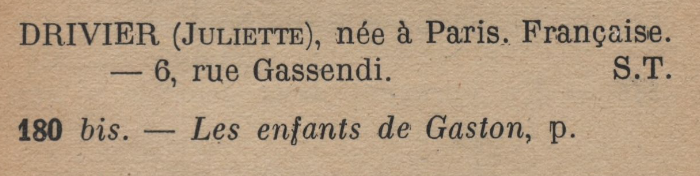
\includegraphics[scale=0.5]{automne1940_2.png} 
		\centering
		\caption{Salon d'automne 1940}
	\end{subfigure}
	\begin{subfigure}{0.5\textwidth}
		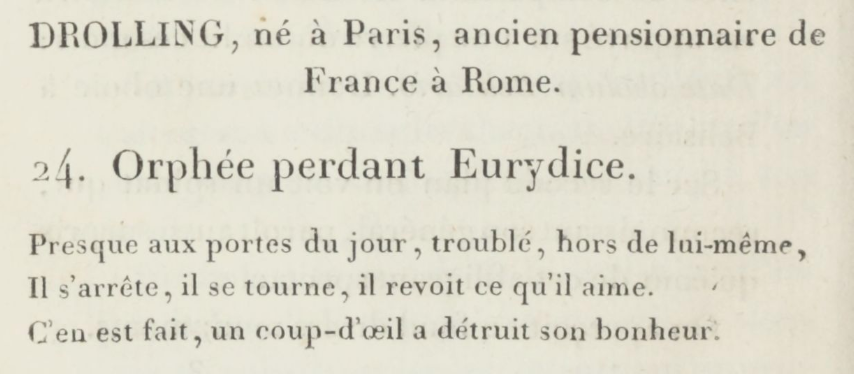
\includegraphics[scale=0.4]{lux1818.png}
		\centering
		\caption{Lux 1818}
	\end{subfigure}
	\begin{subfigure}{0.5\textwidth}
		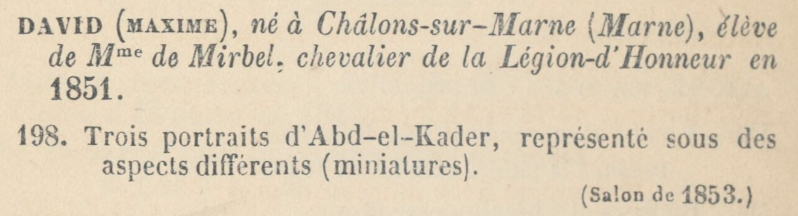
\includegraphics[scale=0.5]{lux1867.png}
		\centering
		\caption{Lux 1867}
	\end{subfigure}
	\begin{subfigure}{0.5\textwidth}
		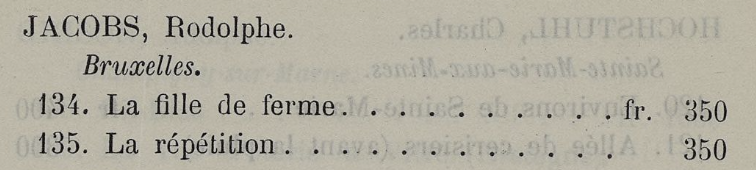
\includegraphics[scale=0.5]{strasbourg1884.png}
		\centering
		\caption{Strasbourg 1884}
	\end{subfigure}
	\begin{subfigure}{0.5\textwidth}
		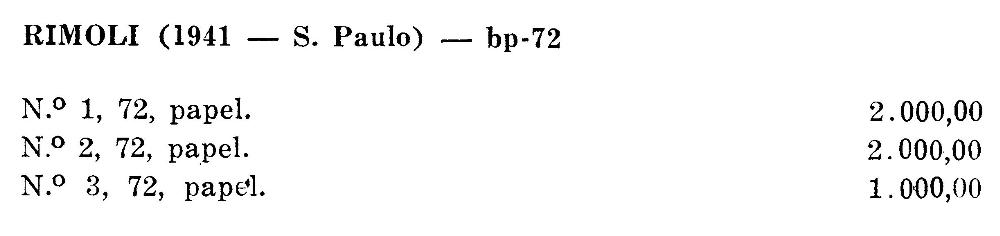
\includegraphics[scale=0.5]{saopaulo1972.png}
		\centering
		\caption{São Paulo 1972}
	\end{subfigure}
	\begin{subfigure}{0.5\textwidth}
		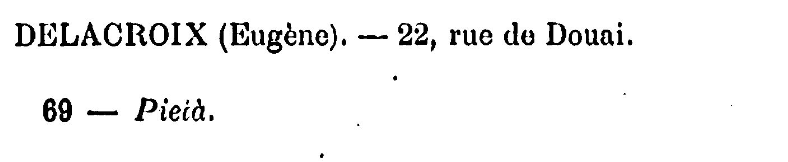
\includegraphics[scale=0.5]{rosecroix1893.png}
		\centering
		\caption{Rose Croix 1893}
	\end{subfigure}
	\begin{subfigure}{0.5\textwidth}
		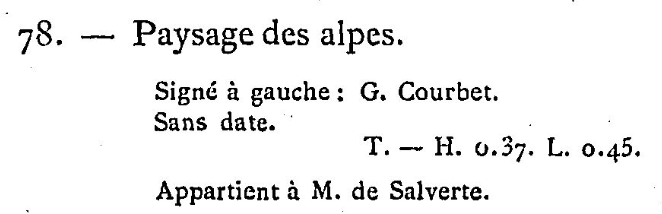
\includegraphics[scale=0.5]{courbet1882.png}
		\centering
		\caption{Courbet 1882}
	\end{subfigure}
\caption{Exemples d'entrées de catalogue (voir annexe B)}
\label{entrees}
\end{figure}


Pour l'œil humain, la structure de ces entrées est évidente. Mais la machine est incapable de déchiffrer ces abstractions visuelles. Il serait envisageable d'entrainer des modèles de segmentation pour analyser la disposition spatiale des lignes (différences dans les marges, emphases typographiques), ou même de calculer leurs disposition à partir des informations encodées en ALTO, afin d'intégrer ce facteur à l'extraction. Cependant, ces démarches s'annoncent hasardeuses et ne semblent pour l'instant absolument pas nécessaires, puisque les regex intégrées au script fonctionnent de manière très satisfaisante. 

Dès lors que l'espace de l'entrée est découpé dans la page, les informations purement textuelles suffisent pour que le script reconstruire l'entrée de manière structurée. Ces catalogues font des usages très spécifiques et différenciés de signes de ponctuation pour organiser leurs informations : points, tirets, virgules, chiffres, etc. En analysant une entrée ligne par ligne, le script  extactionCatalogs détermine à quoi correspond chacune. La première doit normalement présenter un auteur, chose qui est vérifiée avec une regex  dédiée. Les lignes suivantes peuvent être des informations complémentaires, donc le script vérifie à partir de quelle ligne les oeuvres commencent à être signalées : normalement, ces lignes commencent par des numéros. Mais si le numéro est suivi d'une virgule, il s'agit très probablement d'une adresse, et il existe des cas où les œuvres no sont pas numérotées. Postérieurement, il faut séparer dans une même ligne un exposant ou une œuvre de ses informations complémentaires. Le script est désormais capable de traiter tous ces facteurs. Le travail de vérification reste important pour corriger des erreurs qui peuvent parfois être récurrentes, voir nombreuses. Très souvent, il s'agit de problèmes dans la transcription manuelle ou automatique (par exemple, une virgule au lieu d'un point, une lettre "O" au lieu du caractère numérique "0" ont un impact décisif sur la performance du programme). 

Dans certains cas, il est virtuellement possible qu'un utilisateur ait a intégrer ses propres regex dans le fichier \texttt{instantiation\_regex.py}, ce qui est relativement facile à faire. Il suffit de changer les variables \mintinline{bash}|exposant_recuperation_regex| et/ou\\ \texttt{oeuvre\_recuperation\_regex}. Au besoin, l'utilisateur peut aussi modifier les autres regex présentes sur le fichier, qui permettent de détecter des adresses, des mesures, des prix, et des informations complémentaires.


Voici le chemin vers ce fichier : 

\begin{normalsize}
	\begin{minted}{bash}
extractionCatalogs/extractionCatalogs/variables/instanciation_regex.py
	\end{minted}
\end{normalsize}

Il contient toutes les regex utilisées par le script. Voici les plus importantes :\\
\begin{figure}[ht]
	\centering
	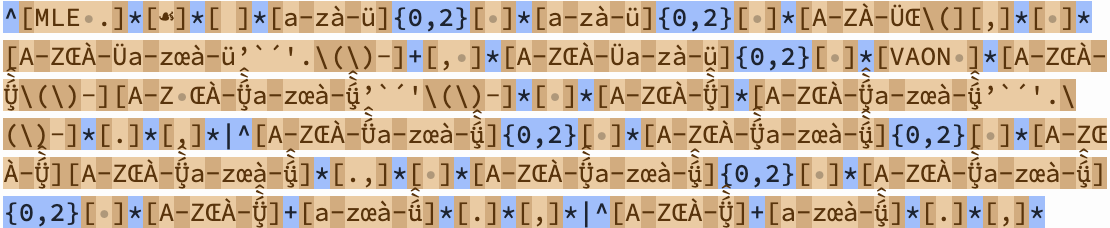
\includegraphics[scale=0.6]{regex_exposant.png}		
	\caption{Regex exposant}
\par
\vspace{1cm}
	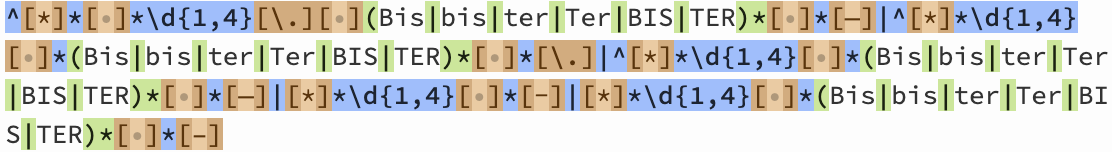
\includegraphics[scale=0.6]{regex_oeuvre.png}		
	\caption{Regex Oeuvre}
\end{figure}

Ces regex ont été développées sur Regex101\footcite{Regex101}, un site gratuit qui permet de construire, de tester et d'expliquer des expressions régulières. Cet outil permet de sauvegarder des tests, que nous pouvons dès lors présenter en action :

\begin{itemize}
\item pour les auteurs : \url{https://regex101.com/r/FCrEk0/1}
\item Pour les œuvres : \url{https://regex101.com/r/hZ1iR3/1}
\end{itemize}

Il faut noter que les exemples d'adresse sont bien écartés au profit des œuvres. Les exemples d'exposants, d'oeuvres et d'adresses sont directement issus du corpus de catalogues Artl@s. D'autres regex mineures restent pour autant fondamentales dans le décryptage des lignes et de leurs informations : 

\begin{itemize}
	\item informations complémentaires :\\ \mintinline{python}|info_comp_regex = re.compile(r'\(.*$,.*$[^0-9.] —.*')|
	\item adresses : \mintinline{python}|regex_adresse = re.compile(r'^[*]*\d{1,4}[ bisBIS]*,')|
	\item mesures : \mintinline{python}|regex_mesures = re.compile(r'^[*]*\d{1,4}[ ]*x')|	
	\item prix : \mintinline{python}|regex_prix = re.compile(r'^[*]*[0-9]+[\.]*[0-9]* fr[ancs]*[.]*')|
\end{itemize}

Si ces expressions régulières permettent de différencier des types d'informations complémentaires, et si elles sont nécessaires pour le fonctionnement du script, celui-ci ne les utilise pas pour encoder ces informations, qui restent sur le niveau de la description. Faute de temps, il n'a pas été possible d'intégrer ces précisions dans la construction de l'arbre TEI, mais le travail est désormais envisageable dans le cadre d'un prochain stage. Il suffira de spécifier des balises où insérer ces informations, et d'adapter les fonctions à cet usage. Par ailleurs, il serait idéal d'intégrer la possibilité d'adapter les regex directement depuis le notebook, en écrivant la variable sur le fichier concerné depuis une cellule. Nous avons fait quelques tests qui, faute de temps, n'ont abouti à rien de concret. 

Malgré l'existence des ces horizons suggérés par les directeurs de stage mais restés que superficiellement explorés, et surtout malgré le fait que dans ce cas spécifique l'efficacité technique l'emporte sur la pédagogie, il est important de mentionner que l'un des piliers de l'efficacité du script réside dans les regex actuellement implémentées.


\section{Informations sur le terminal}

Lors de l'exécution du script, le terminal (ou la cellule Jupyter Notebook) affiche un certain nombre d'informations. Un exemple a été donné dans le chapitre  6.1 (figure 6.1), et peut être consulté en détail en texte brut dans l'annexe C du mémoire.

pour chaque fichier, le terminal imprimera un récapitulatif avec plusieurs indications :

\begin{itemize}
	\item Résultats de la vérification de la conformité à l'ontologie Segmonto
	\item Résultats de restructuration du fichier
	\item Résultats de la vérification de la segmentation saisie manuellement sur eScriptorium, et résultats de la tentative de correction si des erreurs sont détéctées.
	\item Extraction : affichage des entrées complètes sur le terminal	 
\end{itemize}


Suite au traitement de tous les fichier, et de chaque résumé individuel de page, le terminal indiquera un résumé global :
\begin{itemize}
	\item Nombre de pages traitées
	\item Nombre d'entrées extraites
	\item Nombre d'exposants signalés (normalement, le chiffre est égal à celui des entrées)
	\item Nombre d'œuvres extraites
	\item Résultats et problèmes du traitement des fichiers ALTO en input
	\item Résultats et problèmes du fichier TEI produit
	\item Réussite ou échec de création des tableurs CSV
	\item Chemin vers le dossier d'extraction
\end{itemize}


Pour qu'une extraction fonctionne, il n'est pas nécessaire que le processus soit libre d'erreurs. Le script fait tout ce qui lui est possible, et signale des problème que l'utilisateur pourra corriger selon s'il estime que l'extraction est satisfaisante ou pas.

Une extraction de cinq pages du catalogues de Nancy 1843 est proposée dans le guide Jupyter Notebook comme deuxième exemple avec la commande : 
\begin{footnotesize}
	\begin{minted}{bash}
!python3 run.py exemples_guide/Cat_Nancy_1843/ exemples_guide/extractions/ Nancy_1843
	\end{minted}
\end{footnotesize}

Voici en exemple les messages de terminal relatifs à la première page du catalogue, qui ne contient aucune entrée : 

\begin{scriptsize}
	\begin{minted}{bash}

1 – Traitement de Cat_Nancy_1843_typo_0000.xml
		1 – Vérification de la conformité à l'ontologie Segmonto
			[!] L'élément TextBlock (ID='eSc_dummyblock_) du fichier 5_560db_default.jpg n'est pas 
			conforme à l'ontologie Segmonto. 
			[!] Le fichier 5_560db_default.jpg contient un élément TextBlock (ID='eSc_dummyblock_') 
			qui n'est pas associé à l'ontologie Segmonto. [voir attribut TAGREFS]
		2 – Restructuration du fichier
			✓ fichier 'Cat_Nancy_1843_typo_0000.xml_restructuration.xml' créé
		3 – Vérification de l'imbrication des zones saisies sur eScriptorium 
			✓ les lignes et les zones ont été correctement saisies par l'utilisateur/utilisatrice 
		4 – Extraction :



				Ce fichier ne contient pas d'entrées


	\end{minted}
\end{scriptsize}

Voici le résumé final de l'extraction : 
\begin{scriptsize}
	\begin{minted}{bash}
	Résumé :
		6 pages de catalogue traitées [fichiers ALTO]
		25 entrées de catalogue extraites [TextBlocks 'CustomZone:entry']
		25 exposants signalés
		75 oeuvres extraites

	Analyse des fichiers en input [ALTO] :
		[!] 1 fichier non conforme à l'ontologie Segmonto. Consulter le fichier Nancy_1843_problemes.text.
	Analyse du fichier en output [TEI] :
		✓ Le document XML produit est conforme au schéma TEI et à l'ODD du projet.
	Création d'un tableur csv :
		✓ Le fichier csv a été produit

	Chemin du dossier d'extraction : /Users/EstebanSanchez/TNAH_Git/IMAGO-Artl@s/Github_repos/Juliette_Janès/
	IMAGO-Catalogues-Jjanes/extractionCatalogs/exemples_guide/extractions/
	extraction_Nancy_1843
	\end{minted}
\end{scriptsize}\textsl{}

Dans ces deux exemples, le terminal signale des erreurs de conformité à l'ontologie Segmonto. Normalement, si l'utilisateur fait une saisie correcte sur l'interface eScriptorium, cela ne devrait pas avoir lieu, mais l'interaction humaine avec la machine doit rester une source attendue d'erreurs. Dans le catalogue en exemple, ces erreurs n'empêchent pas d'obtenir une extraction très satisfaisante. L'important pour l'utilisateur est d'avoir un retour clair et qu'il soit capable de comprendre ses enjeux. Si l'extraction avait été défaillante, ces informations permettraient de repérer très rapidement les problèmes. Le script permet d'obtenir des informations sur de nombreuses autres types d'erreurs attendues. Une liste exhaustive de ces messages d'erreur peut être consulté en annexe D du mémoire.



\section{Output}

La dernière information sur le terminal rappelle le chemin du dossier produit par le script extractionCatalogs. Celui-ci contient tous les dossiers et fichiers en \texttt{output} :
\begin{itemize}
	\item \texttt{[...].xml} : fichier XML-TEI contenant l'encodage de la totalité des entrées extraites 
	\item \texttt{/CSV} : dossier CSV avec deux tableurs :
	\begin{itemize}
		\item \texttt{[...]\_tableau\_simple.csv} : tableau simplifié pour lecture humaine
		\item \texttt{[...]\_tableau.csv} : tableau adapté en tant qu'input pour la base de donnée BasArt. Il contient de nombreux champs vides et correspond au gabarit du projet.
	\end{itemize}
	\item \texttt{/restructuration ALTO} : dossier avec des fichiers ALTO "restructurés" 
	 "resegmentés". Ils contiennent les corrections des éventuels problèmes de l'\texttt{output} de l'interface eScriptorium. Normalement, ces fichiers n'ont aucune utilité directe pour l'étudiant. Ils permettent tout de même d'approfondir l'usage et la compréhension du script : il est possible de faire des vérifications directement sur ces fichiers.
	\item \texttt{[...]\_problèmes.txt} : fichier de texte brut indiquant des problèmes d'extraction. Ce fichier est produit uniquement dans le cas ou le script n'arrive pas à encoder une ou plus de lignes de texte dans l'arbre TEI.
\end{itemize}


\subsection{Fichier problèmes.txt}

Le fichier \mintinline{bash}|[...]_problemes.txt| permet de signaler les problèmes d'extraction, et notamment les lignes qui n'ont pas été intégrées à l'output TEI. Le script traite chaque ligne, de chaque entrée, de chaque page. Il utilise des regex pour détérminer à quoi correspondent ces lignes, puis les intègre à l'encodage TEI. Il est possible que des lignes ne soient pas reconnues : elles seront ajoutées à ce fichier, avec des indications précises sur leur localisation dans le catalogue (page et ID ou numéro de l'entrée sur le fichier TEI). Le document intégrera aussi les informations générales d'erreur indiquées sur le terminal. Ainsi, l'utilisateur peut localiser très rapidement les erreurs dans l'extraction et les corriger manuellement, que ce soit dans le fichier TEI ou directement dans les tableurs CSV.\\

 Voici un exemple extrait du traitement du catalogue du Salon d'autonmne 1940\footcite{salondautomneCatalogueOuvragesPeinture1940} : 

\begin{footnotesize}
	\begin{minted}{bash}
––––––––––––––––––––––––––––––––––––––––––––
Objets 'entry' avec items non ajoutés au fichier TEI : 
– 'LOMBARD (ALFRED) (voir à ALERED LOMBARD).' (entrée 281)
– 'MALCLES (JEAN-DENIS), né à Paris, Frarçais. — 54, rue Lhomond (Aux Armées). 
 5.4,D.', "394, bis. —  De la, réverie à l'amour", '(composition)' (entrée 297)

––––––––––––––––––––––––––––––––––––––––––––––
Objets 'TextLine' pouvant constituer des lignes de catalogue non ajoutées au fichier TEI 
– 54. (page 97)

––––––––––––––––––––––––––––––––––––––––––––––
Fichiers ALTO en input :
–  Le fichier 42_36c57_default.jpg contient un élément TextBlock
 (ID='eSc_textblock_87e4619f') qui n'est pas associé à l'ontologie Segmonto. 
 [voir attribut TAGREFS]	
	\end{minted}
\end{footnotesize}

On peut observer que ce fichier contient plusieurs sections pour organiser les types d'erreurs possibles. La première indique des entrées entières non ajoutées : ce sont donc des listes contenant plusieurs lignes, qui correspondent généralement à des exposants et leurs œuvres associées. La deuxième section indique qu'une balise \texttt{<TextLine>} dans un fichier ALTO n'a pas été traité en tant que ligne du catalogue : l'utilisateur doit déterminer ce qu'il en est. Dans ce cas, après vérification, on observe rapidement sur l'image de la page qu'il s'agit d'une coquille de transcription automatique.\\

Voici la totalité des sections susceptibles d'apparaître dans le fichier : 
\begin{itemize}
	\item Entrées non intégrées à l'arbre TEI
	\item Zones Segmonto \texttt{CustomZone:entryEnd} non intégrées à l'arbre TEI
	\item Lignes non intégrées à l'arbre TEI
	\item Autres problèmes d'extraction
	\item Problèmes de conformité Segmonto
	\item Problèmes liés à l'input ALTO
\end{itemize}


\subsection{Fichier TEI}

L'\texttt{output} XML TEI est un fichier structuré qui contient un encodage de la totalité des entrées du catalogue qui ont été extraites. L'ODD et le schéma ont été développés par Caroline Corbières pendant le stage Artl@s 2020, et constituait depuis 2019 l\texttt{output} final visé par le pipeline. 

Le \texttt{teiHeader} découle du gabarit nommé \mintinline{bash}|variables/gabarit_teiHeader_IMAGO.py| dans le dossier \texttt{/variables} et peut-être facilement adapté à tout autre projet de recherche. Il y a un gabarit vide nommé \texttt{gabarit\_teiHeader\_vide.py} dans lequel il faut remplir des variables qui correspondent aux balises du \texttt{teiHeader}. Postérieurement, il faut indiquer le nom du gabarit produit sur la seule ligne de code du fichier \mintinline{bash}|variables/contenu_tei.py|.
Ainsi, des étudiants ou des chercheurs travaillant hors du cadre du projet Artl@s peuvent produire très facilement des encodages adaptés à leurs besoins. C'est le cas de Frédérine Corbières, étudiante du certificat en humanités numériques de l'Unige, qui a travaillé sur l'encodage de catalogues pictorialistes de la fin du XIXe siècle, et dont le gabarit \texttt{gabarit\_teiHeader\_PictoCatalogs.py} est inclu à titre d'exemple dans le dossier.

Toutes les entrées du catalogue se trouvent dans la balise \mintinline{xml}|<body>| du fichier, à l'intérieur de la balise \mintinline{xml}|<list>|.
Une entrée est contenue dans une balise \mintinline{xml}|<entry>|, laquelle est numérotée, possède un attribut ID, et contient un lien vers la découpe de l'image iiif (si celle-ci existe). Une balise \mintinline{xml}|<desc>| (description) contient le nom de l'exposant (balise \mintinline{xml}|<name>|) et ses informations complémentaires (balise \mintinline{xml}|<trait>| et \mintinline{xml}|<p>|). Suivent des balises \mintinline{xml}|<item>|, qui sont numérotées et possèdent un attribut ID. Elles contiennent le numéro de l'œuvre (balise \mintinline{xml}|<num>|), son titre (balise \mintinline{xml}|<title>|) et son éventuelle description (balise \mintinline{xml}|<desc>|).\\

Voici un exemple d'entrée issue du catalogue Nancy 1843 :
\begin{footnotesize}
	\begin{minted}{xml}
<entry n="1" xml:id="Nancy_1843_e1" source="https://gallica.bnf.fr/iiif/ark:/12148/[...]>
	<desc>
		<name>M.ANDRÉ,</name>
		<trait>
			<p> peintre, rue des Carmes, à Nancy.</p>
		</trait>
	</desc>
	<item n="1" xml:id="Nancy_1843_e1_i1">
		<num>1</num>
		<title>Portrait de M.D.V...... </title>
		<desc>(pastel).</desc>
	</item>
	<item n="2" xml:id="Nancy_1843_e1_i2">
		<num>2</num>
		<title>Idem de M. C. J...., idem.</title>
		<desc>idem.</desc>
	</item>
		<item n="3" xml:id="Nancy_1843_e1_i3">
		<num>3</num>
		<title>L'Aumône, idem.</title>
		<desc>idem.</desc>
	</item>
		<item n="4" xml:id="Nancy_1843_e1_i4">
		<num>4</num>
		<title>Portrait de M. C...., idem.</title>
		<desc>idem.</desc>
	</item>
		<item n="5" xml:id="Nancy_1843_e1_i5">
		<num>5</num>
		<title>Idem de M. H....., idem.</title>
		<desc>idem.</desc>
	</item>
</entry>
	\end{minted}
\end{footnotesize}



\subsection{Fichiers CSV}

Le stage 2022 a intégrée une dernière étape au pipeline, afin de produire des instruments structurés lisibles par des êtres humains et immédiatement injectables à la base de données BasArt. Il s'agit de produire deux tableurs CSV (Comma Separated Value) contenant la totalité des informations extraites, à partir du fichier TEI. Le script extractionCatalogs utilise pour cela deux feuilles de transformations XSL : \texttt{XMLtoCSV.xsl} et \texttt{XMLtoCSVsimple.xsl}. La structure de ces feuilles de transformation est issue du travail de Ljudmila Petkovic pour le projet Artl@s en 2019. Il a été question d'adapter la feuille à nos besoins (noms des champs, cellules supplémentaires) et de l'intégrer au script python. 

Voici les fichiers produits : 
\begin{itemize}
\item \texttt{[...]\_tableau\_simple.csv} : Une version simplifiée permet de lire facilement ces informations, afin de vérifier lesquelles doivent être corrigées manuellement.

\item \texttt{[...]\_tableau.csv} : Une version complète et adaptée au cahiers des charges de la base de données BasArt du projet Artl@S.
\end{itemize}

Ce dernier fichier peut alimenter directement la base à travers du site dédié, moyennant une intervention manuelle. L'utilisateur doit l'ouvrir et compléter deux cellules qui se situent en haut à gauche :

\begin{figure}[ht]
	\centering
	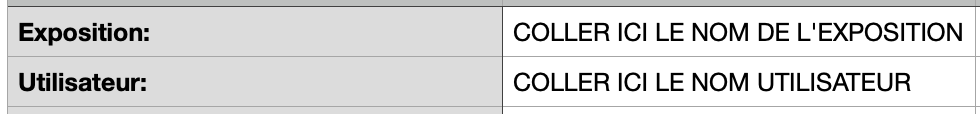
\includegraphics[scale=0.6]{csv.png}		
	\caption{Tableau CSV : cellules à remplir}
\end{figure}

Les étudiants du certificat en humanités numériques possèdent normalement un compte utilisateur BasArt (https://artlas.huma-num.fr/fr/bases-en-acces-libre/ ) :
\begin{itemize}
	\item Ils doivent copier/coller ce nom d'utilisateur dans la cellule \texttt{COLLER ICI LE NOM UTILISATEUR}
	
	\item Puis rechercher le nom de l'exposition/catalogue sur la base, et copier/coller le nom de l'exposition/catalogue dans la cellule  \texttt{COLLER ICI LE NOM DE L'EXPOSITION}
	
	\item Ils peuvent finalement utiliser un formulaire dédié pour envoyer leur tableur CSV
\end{itemize}

Ces manipulations permettent qu'un travail produit dans un cadre scolaire alimente directement une base de données connue et amplement utilisée comme instrument de recherche dans le milieu de l'histoire de l'art.


\section{Corrections manuelles}

Les interventions et les corrections manuelles font partie intégrante du pipeline et peuvent avoir lieu, selon les besoins et les aptitudes de chaque utilisateur, à toutes les étapes du processus. Il est possible d'intervenir sur tous les documents, mais un étudiant débutant pourra se limiter à l'interface eScriptorium et à l'\texttt{output} CSV.

\begin{itemize}
	\item Sur l'interface eScriptorium, l'utilisateur peut produire manuellement ou automatiquement les transcriptions et les segmentations. L'interface permet aussi de faire toutes les corrections nécessaires sur la page d'édition dédiée
	
	\item Sur les fichiers XML ALTO produits par eScriptorium, l'utilisateur peut corriger la transcription automatique, le découpage des zones, ainsi que leur conformité à l'ontologie Segmonto. Ces corrections peuvent être faites sur eScriptorium, mais un utilisateur expérimenté gagnera beaucoup de temps en traitant directement les fichiers ALTO
	
	\item Le script python extractionCatalogs est librement adaptable aux besoins des utilisateurs. Les manipulations plus simples et attendues sont l'intégration d'expressions régulières au fichier \texttt{instanciation\_regex.py} et la création de gabarits personnalisés pour le \texttt{teiHeader} de projets spécifiques. Un utilisateur avec des connaissances intermédiaires en programmation pourra s'appuyer sur les nombreux commentaires pour modifier le code selon ses besoins
	
	\item Sur le fichier XML TEI en \texttt{output}, l'utilisateur peut corriger le contenu et la structure des entrées : numéros, texte, attributs, etc. Il pourra ainsi s'assurer d'avoir des encodages bien formés, mais cela n'est pas indispensable pour produire les fichiers CSV
	
	\item sur les fichiers CSV en \texttt{output}, l'utilisateur peut corriger le contenu et la structure des entrées
\end{itemize}

Éditer des fichiers XML peut être difficile pour un.e utilisateur/utilisatrice néophyte. Il faut savoir lire un document complexe et veiller à ce que sa conformité sot respectée. Si un logiciel comme Oxygen permet de faire cela de manière efficace, celui-ci est payant et n'est en conséquence pas conforme à un cahier des charges fondé sur les principes de la science ouverte. Notons seulement que les institutions de recherche possèdent souvent des licences pour utiliser ce logiciel, et que les essais gratuits sont très faciles à obtenir. 

L'utilisateur doit utiliser les informations imprimées sur le terminal et sur le fichier \texttt{[...]\_problèmes.txt} pour détecter rapidement les corrections à faire. Il s'agira de corriger des problèmes de transcription, mais aussi d'ajouter des auteurs, des œuvres ou des informations complémentaires exclues pendant l'extraction.

Il est important de noter que les modifications sur les documents XML en \texttt{input} (ALTO) et en \texttt{output} (TEI) impliqueront que la même commande remplace les résultats antérieurs (si les mêmes chemins et le même titre de catalogue sont indiqués). Quant aux fichiers XML intermédiaires de "restructuration" et de "resegmentation", ils sont produits sur la base des ALTO en \texttt{input} et leur modification n'affectera en rien les résultats de l'exécution de la même commande. Cependant, dans ce cas, le terminal affichera un message demandant si l'utilisateur veut remplacer les versions modifiées/anciennes. Sur Jupyter Notebook, toutefois, l'utilisateur ne pourra pas faire ce choix car le message de terminal n'accepte pas d'\texttt{input} : il faudra changer systématiquement le nom de catalogue et/ou le chemins d'\texttt{output} quand des modifications sont réalisées sur les fichiers ALTO ou TEI. Comme indiqué, cela ne sera pas un problème pour l'usage normal d'un étudiant : seule des interventions plus poussées nécessitent donc de l'utilisation d'un terminal. 

Le guide Jupyter Notebook conclut en proposant à l'utilisateur plusieurs exemples de commandes pour transcrire des catalogues. Ils fournissent des cas concrets d'erreurs récurrentes qui ne nuisent pas à l'extraction satisfaisante des entrées. Elles peuvent être lancées directement sur le notebook ou bien sur un terminal \texttt{bash}, en se déplaçant sur le dossier \texttt{/extractionCatalogs} et en enlevant le signe préalable [\texttt{!}] : 

\begin{scriptsize}
	\begin{minted}{bash}
!python3 exemples_guide/Cat_Automne_1940/ exemples_guide/extractions/ automne_1940

!python3 run.py exemples_guide/Cat_Refuses_1863/ exemples_guide/extractions/ refuses_1863

!python3 run.py exemples_guide/Cat_Rouen_1853/ exemples_guide/extractions/ rouen_1853

!python3 run.py exemples_guide/Cat_Strasbourg_1884/ exemples_guide/extractions/ Strasbourg_1884

!python3 run.py exemples_guide/PCP_1896/ exemples_guide/extractions/ PCP_1896

!python3 run.py exemples_guide/Cat_SaoPaulo_1972/ exemples_guide/extractions/ saopaulo_1972
	\end{minted}
\end{scriptsize}



% EXEMPLES MINTED			
\begin{comment}
	\begin{scriptsize}
		\begin{minted}{bash}
			
		\end{minted}
	\end{scriptsize}
	
	\begin{minted}{python}
		def boring(truc):
		pass
	\end{minted}
	
	\begin{minted}{xml}
		\centering
		<entry n="1" xml:id="Nancy_1843_e1" 
		<desc>
		<name>M.ANDRÉ,</name>
		<trait>
		<p> peintre, rue des Carmes, à Nancy.</p>
		</trait>
		</desc>
		<item n="1" xml:id="Nancy_1843_e1_i1">
		<num>1</num>
		<title>Portrait de M.D.V...... </title>
		<desc>(pastel).</desc>
		</item>
	\end{minted}
	
	
	
	\begin{minted}{bash}
		!python3 run.py exemples_guide/Cat_Automne_1940/exemples_guide/extractions/ automne_1940
		
	\end{minted}
	
	Texte \mintinline{bash}{automne_1940} Continuation du texte
	X\mintinline{python}{print(x**2)}X
	\mint{python}|import this|
	\mint{python}|for x in truc:|	
	%\inputminted[⟨options⟩]{⟨language⟩}{⟨filename⟩}.
	
\end{comment}


\chapter*{Conclusion}
\addcontentsline{toc}{chapter}{Conclusion}


%	-récapituler ce qui a été fait et écrit (sans se répéter) 

Le présent mémoire a proposé un bilan réflexif pour un stage dont les enjeux font écho aux transformations que le numérique opère sur la recherche en sciences humaines. Il a suggéré que ces enjeux, organiquement reliés, étaient a situer sur des plans épistémologiques, institutionnels et pédagogiques. Les questionnements formulés ont permis de comprendre aussi bien  que de définir la signification scientifique du travail effectué et sa vocation pédagogique. En tant que synthèse et chronique abordant le processus par ses dimensions intellectuelles, techniques et logistiques, ce mémoire a aussi permis d'élucider le positionnement résolument technicien de la mission, et de la situer dans le paysage académique des humanités numériques. 

À partir d'une structure allant du général vers le particulier, nous avons commencé par explorer les enjeux profonds du stage et cheminé vers les aspects purement logistiques et techniques du livrable final. L'introduction présente ses implications scientifiques, techniques et pédagogiques sous un prisme issu de la sociologie et de l'histoire des sciences. Il s'agit premièrement de comprendre les cadres qui donnent sens au stage, et d'exposer les frontières mouvantes d'un travail collaboratif qui implique des chercheurs, des étudiants et des ingénieurs. Puis de réfléchir aux conséquences d'une transposition du catalogue papier vers des supports numériques qui démultiplient les traitements possibles de ses informations et font éclater son unité documentaire. Nous suggérons que ces tensions, à défaut de pouvoir être résolues, permettent de construire des approches rigoureuses.

La première partie décrit les enjeux scientifiques et logistiques du travail en le positionnant dans un historique constitué par quatre stages depuis 2019. Elle commence par une chronique des missions antérieures qui fait état des continuités et des ruptures dans le projet global ; cette synthèse peut servir à des futurs collaborateurs pour définir des directions à prendre à l'avenir. Un premier stage en 2019 a posé les bases avec une réflexion sur l'utilité de l'encodage automatique de catalogues du XIXe siècle. Il a conclu avec une première chaîne de traitement mettant au centre les logiciels Transkribus (reconnaissance de caractères) et Grobid (encodage automatique des entrées). En 2020, le \textit{workflow} a été systématisé pour servir à des corpus plus amples, et une réflexion sur l'encodage des catalogues a abouti à la création d'une ODD solide. En 2021, le pipeline a été transformé dans son ensemble pour transposer les données vers des logiciels conformes à la science ouverte (eScriptorium, kraken, python) : les enjeux étaient la gratuité, la transparence et la reproductibilité des méthodes. À l'aune du stage 2022, deux défauts étaient manifestes : la complexification de la chaîne au nom de l'efficience la rendait absolument inutilisable par des collaborateurs sans aptitudes techniques préalables ; de plus, ces chaînes impliquaient des interventions conséquentes qui mettaient en cause leur caractère "automatique", voire "semi-automatique". La mission s'est donc tourné vers un objectif éminemment pédagogique, et a consisté à construire un outil simple et solide. 

La deuxième partie du mémoire décrit en détail l'utilisation de la chaîne de traitement résultante, et s'attarde dans le fonctionnement du script python qui permet l'encodage des catalogues. Il s'agit d'un pipeline en deux étapes abordables par des néophytes. La première repose dans l'utilisation de l'interface eScriptorium pour produire des transcriptions ALTO à partir des catalogues numérisées. La deuxième se limite à l'exécution du script extractionCatalogs à travers d'un notebook Jupyter, qui sert d'interface d'utilisation en mênme temps que de guide. Les interventions intermédiaires se réduisent au téléchargement de fichiers et à leur positionnement dans des dossiers souhaités. Nous considérons que cela constitue une amélioration conséquente face aux conditions antérieures, qui impliquaient de nombreuses étapes médiées par des interventions hasardeuses (utilisation du terminal, commandes confuses, transformations XSL des fichiers, prise en main de logiciels complexes, instructions difficiles). Un autre apport réside dans l'éloquence du script : outre le fait qu'il soit amplement documenté (dans le mémoire, dans le notebook et dans les fichiers \texttt{.py}), il produit des message de réussite et d'erreur conçus pour que l'utilisateur comprenne les résultats, même quand ceux-ci ne sont pas satisfaisants.

Le pipeline semi-automatique extractionCatalogs (océrisation avec eScriptorium + extraction avec le script extractionCatalogs), accompagné par une interface et guide d'utilisation (Jupyter notebook), a donc un intêret scientifique (produire des données pour la recherche), technique (produire efficacement ces données) et pédagogique (présenter des technologies numériques fondamentales dans le domaine des humanités numériques). Nous éstimons que la priorité donnée à l'enseignement face à l'efficacité ne remet pas en question l'utilité pragmatique du pipeline. Pour la première fois, Artl@s compte avec un outil qui peut être véritablement déployé par ses collaborateurs, et il est virtuellement possible que cela ait un impact sur l'enrichissement de la base de données BasArt.\\

Au delà, il reste à faire un bilan concret sur l'instrument développé, avec son utilisation dans le cadre des cours d'initiation aux humanités numériques de Béatrice Joyeux-Prunel. Nous sommes invités à intervenir à l'université de Genève pendant l'année scolaire 2022-2023 pour accompagner les étudiants dans l'utilisation du pipeline. Cela nous permettra de contribuer à l'évaluation de l'outil, voire à une définition des problématiques possibles pour la continuation du projet avec un stage en 2023. Nous pouvons rappeler pour l'instant, à travers de l'image de "l'ingénieur lettré", que notre rôle a impliqué de doubler au développement de nos aptitudes numériques une compréhension profonde des enjeux scientifiques et pédagogiques du projet. Nous pouvons dès lors chercher les angles morts du stage 2022, et nous demander s'il existe des solutions plus efficaces pour équilibrer les pôles différenciés que constituent ses objectifs. Nous pourrions commencer par interroger ces instruments nouveaux pour savoir s'ils imposent des pertes, des lacunes, et ne pas oublier que les catalogues traités, en tant qu'unités intellectuelles et matérielles, constituent des traces historiques lourdes en significations face auxquelles le numérique ne saurait se substituer. 


%les annexes
\appendix
\chapter{liste des améliorations dans le script python}
Cette liste concerne des améliorations ou des corrections effectuées sur le prototype de script python de 2021. 

\begin{itemize}
	\item Exclusion des fichiers autres que ALTO et des fichiers/dossiers  cachés dans le dossier en \texttt{input} (permet entre autres l'utilisation de MacOS avec l'omission du dossier \texttt{.DS\_Store}). Cela permet d'avoir des dossiers contenant des images ou d'autres types de fichiers
	\item Exclusion des fichiers ALTO restructurés : la commande peut être exécutée plusieurs fois en évitant la multiplication en boucle des restructurations
	\item Tabulations et précisions sur le terminal pour rendre les messages plus lisibles avec une visualisation structurée des entrées
	\item Le fichier TEI en \texttt{output} est correctement indenté. Il contient des commentaires pour guider la saisie du \texttt{teiHeader}
	\item \texttt{teiHeader} produit en avec la librairie \texttt{lxml} est désormais conforme (l'arbre produit contenait plusieurs erreurs d'imbrication)
	\item simplification du fichier de création \texttt{teiHeader} : variables renommées, refactorisées, réordonnées 
	\item restructuration et refactorisation des dossiers du script dans le dossier \texttt{/extractionCatalogs} pour plus de clarté 
	\item Ajout de commentaires nombreux et détaillés sur le script pour guider l'utilisateur dans un but pédagogique
	\item Réécriture du README et des commentaires déjà existants pour plus de clarté
	\item Creátion de gabarits interchangeables pour les information fondamentales du \texttt{teiHeader} (dossier \texttt{/variables})
	\item les fichier restructurés sont désormais placés dans un dossier dédié \texttt{restructuration}, et non plus dans le dossier des fichiers en \texttt{input}
	\item Lorsqu'un des ALTO en \texttt{input} a déjà subi une restructuration, le terminal averti que le fichier produit sera pareil et demande si l'on veut continuer. Si ce n'est pas le cas, le fichier n'est pas restructuré une deuxième fois, et l'ALTO en \texttt{input} déjà structuré est utilisé à sa place 
	\item si le catalogue est issu d'un manifeste iiif : le terminal affiche un lien vers une découpe des zones de chaque entrée du catalogue
	\item Il n'est plus nécessaire d'intervenir sur le code pour désactiver les fonctions relatives aux zones Segmonto \texttt{CustomZone:entryEnd} si le catalogue n'en a pas
	\item le pipeline ignore les régions vides dans la transcription ALTO, qui sont souvent des erreurs de segmentation sur eScriptorium. Cela permet de ne pas générer des entrées vides qui nuisent à la conformité et à la structure de l'\texttt{output} TEI (la numérotation résultait inexacte).
	\item Lorsque la segmentation d'un fichier n'est pas conforme à l'ontologie Segmonto, un message sur le terminal l'indique et renvoie vers le répositoire Segmonto 
	\item Le terminal indique si un fichier traité ne contient pas d'entrées (c'est par exemple le cas pour une page de titre)
	\item Le terminal affiche le nombre total d'entrées extraites. Si aucune entrée n'est extraite des fichiers restructurés, le terminal affiche qu'il s'agit peut être d'une erreur de construction des expressions régulières ou de conformité à l'ontologie Segmonto
	\item les noms des fichiers ALTO peuvent avoir ou ne pas avoir des "zéros non significatifs" (ex:  "9" ou "09"), ils seront traités dans tous les cas dans l'ordre correct
	\item le fichier de problèmes \texttt{[...]\_problèmes.txt} indique maintenant si les items sont des \texttt{CustomZone:entryEnd} ou des \texttt{CustomZone:entry}
	\item le terminal comporte un résumé qui indique : 
	\begin{itemize}
		\item nombre d'entrées extraites
		\item nombre d'auteurs signalés
		\item nombre d'auteurs non signalés (et ID des entrées concernées)
		\item nombre d'œuvres extraites
	\end{itemize}
	\item la commande "-v" pour vérifier la conformité des fichiers ALTO est maintenant fonctionnelle. Elle vérifie si une une \texttt{TextLine} se trouve directement dans un \texttt{TextBLock} associé à une zone Segmonto \texttt{MainZone} et non pas à une \texttt{CustomZone:entry} (ce problème est inhérent à eScriptorium et rend l'extraction impossible). La commande affiche aussi s'il y a des erreurs de conformité ALTO ou à l'ontologie Segmonto
	\item Les items avec plusieurs lignes sont traités correctement
	\item L'utilisateur n'a plus besoin d'intervenir sur le script pour adapter les expressions régulières à son catalogue. Les regex implémentées sont normalement capables de gérer la très grande majorité des cas possibles
	\item Les adresses sont correctement différenciées des items
	\item Items "bis" pris en compte pour ne pas nuire à la conformité TEI
	\item le document \texttt{[...]\_problèmes.txt} est désormais divisé en parties : auteurs non signalés, \texttt{CustomZone:entry} non ajoutées, \texttt{CustomZone:entryEnd} non ajoutées, récapitulatif général des erreurs
	\item Dans l'\texttt{output} TEI, les balises de description \texttt{<trait>} et \texttt{<p>} ne sont créés que si l'entrée contient une description
	\item Commandes obligatoires de définition du type du catalogue éliminées : "Nulle",  "Triple", "Double", "Simple" : le script détecte automatiquement le type de catalogue
	\item Le terminal affiche maintenant les description des œuvres
	\item Le script capable de reconnaitre des des œuvres dans des catalogues où ceux-ci ne sont pas numérotés
	\item Étape supplémentaire : le script opère deux transformations XSL et produit deux tableurs CSV à partir du fichier TEI	
\end{itemize}



\chapter{Échantillons d'entrées de catalogue}	
Chaque échantillon a été sélectionné au hasard dans chacun des catalogues du corpus traité. En résultent des exemples très représentatifs, avec quelques exceptions que le script extractionCatalogs est capable de traiter correctement\textsl{}.\\
 
La découpe de l'image correspond à la région \texttt{CustomZone:entry} de l'ontologie Segmonto.\\
\textsl{}
Les références complètes de chaque catalogue peuvent être trouvées dans la Bibliographie, dans la section "Catalogues traités (corpus Artl@s)".
L'objectif de cet annexe est d'offrir des repères visuels généraux au lecteur,\textsl{} et la sélection n'a pas suivi aucun protocole particulier d'échantillonnage. 



	\begin{figure}
		\begin{subfigure}{0.5\textwidth}
			\includegraphics[scale=0.5]{inde1892.png}
			\centering
			\caption{Salon des Indépendants 1892}
		\end{subfigure}
		\begin{subfigure}{0.5\textwidth}
			\includegraphics[scale=0.5]{inde1913.png}
			\centering
			\caption{Salon des Indépendants 1913}
		\end{subfigure}
		\begin{subfigure}{0.5\textwidth}
			\includegraphics[scale=0.4]{inde1923.png}
			\centering
			\caption{Salon des Indépendants 1923}
		\end{subfigure}
		\begin{subfigure}{0.5\textwidth}
		\includegraphics[scale=0.5]{inde1935.png}
		\centering
		\caption{Salon des Indépendants 1935}
	\end{subfigure}
			\caption{Salon des Indépendants}
	\end{figure}
	
	\begin{figure}	
		\begin{subfigure}{0.5\textwidth}
			\includegraphics[scale=0.5]{nancy1843.png}
			\centering
			\caption{Nancy 1843}
		\end{subfigure}
		\begin{subfigure}{0.5\textwidth}
			\includegraphics[scale=0.5]{nancy1892.png}
			\centering
			\caption{Nancy 1892}
		\end{subfigure}
		\begin{subfigure}{0.5\textwidth}
			\includegraphics[scale=0.4]{nancy1849.png}
			\centering
			\caption{Nancy 1849}
		\end{subfigure}	
	\caption{Société lorraine des amis des arts}
	\end{figure}
	
	\begin{figure}
		\begin{subfigure}{0.5\textwidth}
		\includegraphics[scale=0.4]{paris1961.png}
		\centering
		\caption{Paris 1961}
	\end{subfigure}
		\begin{subfigure}{0.5\textwidth}
		\includegraphics[scale=0.5]{paris1965.png}
		\centering
		\caption{Paris 1965}
	\end{subfigure}
		\begin{subfigure}{0.5\textwidth}
		\includegraphics[scale=0.5]{paris1969.png}
		\centering
		\caption{Paris 1969}
	\end{subfigure}
	\caption{Paris}
	\end{figure}
	
	
	
	\begin{figure}
	
		\begin{subfigure}{0.5\textwidth}
		\includegraphics[scale=0.5]{rouen1853.png}
		\centering
		\caption{Rouen 1853}
	\end{subfigure}
		\begin{subfigure}{0.5\textwidth}
		\includegraphics[scale=0.5]{rouen1856.png}
		\centering
		\caption{Rouen 1856}
	\end{subfigure}
		\begin{subfigure}{0.5\textwidth}
		\includegraphics[scale=0.5]{rouen1860.png}
		\centering
		\caption{Rouen 1860}
	\end{subfigure}
		\begin{subfigure}{0.5\textwidth}
		\includegraphics[scale=0.5]{rouen1869.png}
		\centering
		\caption{Rouen 1869}
	\end{subfigure}
		\begin{subfigure}{0.5\textwidth}
		\includegraphics[scale=0.5]{rouen1872.png}
		\centering
		\caption{Rouen 1872}
	\end{subfigure}
		\begin{subfigure}{0.5\textwidth}
		\includegraphics[scale=0.5]{rouen1878.png}
		\centering
		\caption{Rouen 1878}
	\end{subfigure}
		\begin{subfigure}{0.5\textwidth}
		\includegraphics[scale=0.5]{rouen1888.png}
		\centering
		\caption{Rouen 1888}
	\end{subfigure}
		\begin{subfigure}{0.5\textwidth}
		\includegraphics[scale=0.5]{rouen1891.png}
		\centering
		\caption{Rouen 1891}
	\end{subfigure}
		\begin{subfigure}{0.5\textwidth}
		\includegraphics[scale=0.5]{rouen1895.png}
		\centering
		\caption{Rouen 1895}
	\end{subfigure}
		\begin{subfigure}{0.5\textwidth}
		\includegraphics[scale=0.5]{saopaulo1851.png}
		\centering
		\caption{Rouen 1851}
	\end{subfigure}
	\caption{Exposition annuelle du musée de Rouen}
	\end{figure}
	
	
	
	\begin{figure}
		\begin{subfigure}{0.5\textwidth}
		\includegraphics[scale=0.5]{venezia1895.png}
		\centering
		\caption{Venezia 1895}
	\end{subfigure}
		\begin{subfigure}{0.5\textwidth}
		\includegraphics[scale=0.5]{venezia1905.png}
		\centering
		\caption{Venezia 1905}
	\end{subfigure}
		\begin{subfigure}{0.5\textwidth}
		\includegraphics[scale=0.5]{venezia1920.png}
		\centering
		\caption{Venezia 1920}
	\end{subfigure}
	\caption{Bienale de Venise}
	\end{figure}
	
	
	
	\begin{figure}	
		\begin{subfigure}{0.5\textwidth}
			\includegraphics[scale=0.5]{PCP1894.png}
			\centering
			\caption{PCP 1894}
		\end{subfigure}
			\begin{subfigure}{0.5\textwidth}
			\includegraphics[scale=0.5]{PCP1896.png}
			\centering
			\caption{PCP 1896}
		\end{subfigure}
			\begin{subfigure}{0.5\textwidth}
			\includegraphics[scale=0.5]{PCP1898.png}
			\centering
			\caption{PCP 1898}
		\end{subfigure}
			\begin{subfigure}{0.5\textwidth}
			\includegraphics[scale=0.5]{PCP1902.png}
			\centering
			\caption{PCP 1902}
		\end{subfigure}
		\begin{subfigure}{0.5\textwidth}
		\includegraphics[scale=0.5]{PCP1904.png}
		\centering
		\caption{PCP 1904}
		\end{subfigure}
		\begin{subfigure}{0.5\textwidth}
		\includegraphics[scale=0.4]{PCP1906.png}
		\centering
		\caption{PCP 1906}
		\end{subfigure}
	\caption{Photo Club Paris (PCP)}
	\end{figure}
	
	
	
	
	\begin{figure}[ht]
	\begin{subfigure}{0.5\textwidth}
		\includegraphics[scale=0.5]{automne1940.png	} 
		\centering
		\caption{Salon d'automne 1940}
	\end{subfigure}
	\begin{subfigure}{0.5\textwidth}
	\includegraphics[scale=0.5]{automne1940_2.png	} 
	\centering
	\caption{Salon d'automne 1940}
\end{subfigure}
	\begin{subfigure}{0.5\textwidth}
		\includegraphics[scale=0.4]{lux1818.png}
		\centering
		\caption{Lux 1818}
	\end{subfigure}
	\begin{subfigure}{0.5\textwidth}
		\includegraphics[scale=0.5]{lux1867.png}
		\centering
		\caption{Lux 1867}
	\end{subfigure}
	\begin{subfigure}{0.5\textwidth}
		\includegraphics[scale=0.5]{strasbourg1884.png}
		\centering
		\caption{Strasbourg 1884}
	\end{subfigure}
	\begin{subfigure}{0.5\textwidth}
	\includegraphics[scale=0.5]{saopaulo1972.png}
	\centering
	\caption{São Paulo 1972}
\end{subfigure}
	\begin{subfigure}{0.5\textwidth}
	\includegraphics[scale=0.5]{rosecroix1893.png}
	\centering
	\caption{Rose Croix 1893}
\end{subfigure}
\begin{subfigure}{0.5\textwidth}
	\includegraphics[scale=0.5]{courbet1882.png}
	\centering
	\caption{Courbet 1882}
\end{subfigure}


	\caption{Catalogues non groupés}
	
\end{figure}


\chapter{Informations de terminal pour une page de catalogue extraite}

L'exemple ci dessus est issu de la première page contenant des entrées du catalogue du Salon de Nancy 1843.\footcite{societelorrainedesamisdesartsCataloguePeinturesMiniatures1843}

\begin{scriptsize}
	\begin{minted}{bash}
		
==============================================
1 – Traitement de Cat_Nancy_1843_typo_0001.xml
	1 – Vérification de la conformité à l'ontologie Segmonto
		✓ le fichier issu d'eScriptorium est conforme à l'ontologie Segmonto
	2 – Restructuration du fichier
		✓ fichier 'Cat_Nancy_1843_typo_0001.xml_restructuration.xml' créé
	3 – Vérification de l'imbrication des zones saisies sur eScriptorium 
		Le Ficher Alto produit par eScriptorium contient des zones ['TextBLock'] vides
		– Parmi ces zones ['TextBlock'] vides, il y a des 'CustomZone:entry'
		✓ Correction automatique : 18 lignes correspondant à 2 zones vides ont été déplacées vers ces zones
	4 – Extraction :


			M.ANDRÉ,
			 peintre, rue des Carmes, à Nancy.
				1. Portrait de M.D.V...... 
					(pastel).
				2. Idem de M. C. J...., idem.
					idem.
				3. L'Aumône, idem.
					idem.
				4. Portrait de M. C...., idem.
					idem.
				5. Idem de M. H....., idem.
					idem.
				6. La Sorcière. idem.
				7. Portrait de M....... 
					(pastel.)
				Image : 		https://gallica.bnf.fr/iiif/ark:/12148/bpt6k62251805/f7/
				217.0,1320.0,1333.0,735.0/full/0/default.jpg
			M. ANDRÉ JEUNE,
			 professeur de dessin de machines, 11, rue de la Pépinière.
				8. Locomotive 
					(dessin au lavis).
				9. Machine, idem.
				idem.
				10. Pont de Suresnes.
				11. La Chapelle de Notre-de-Dame des flammes même de 	 	
				l'évènement du 8 mai.
				Image : https://gallica.bnf.fr/iiif/ark:/12148/bpt6k62251805/f7/
				203.0,2079.0,1354.0,714.0/full/0/default.jpg
				


==============================================
	Résumé :
		1 page de catalogue traitée [fichier ALTO]
		2 entrées de catalogue extraites [TextBlocks 'CustomZone:entry']
		2 exposants signalés
		11 oeuvres extraites

	Analyse des fichiers en input [ALTO] :
		✓ La segmentation des pages est conforme à l'ontologie Segmonto
	Analyse du fichier en output [TEI] :
		✓ Le document XML produit est conforme au schéma TEI et à l'ODD du projet.
	Création d'un tableur csv :
		✓ Le fichier csv a été produit
	
	Chemin du dossier d'extraction : /Users/EstebanSanchez/TNAH_Git/IMAGO-Artl@s/Github_repos/Juliette_Janès/
	IMAGO-Catalogues-Jjanes/extractionCatalogs/exemples_guide/extractions/
	extraction_Nancy_1843_page

		
	\end{minted}
\end{scriptsize}

\chapter{Liste des erreurs affichables par le terminal}

\begin{itemize}
	\item \texttt{[!] ATTENTION : ce fichier avait déjà été restructuré ; le nouveau fichier produit est identique."}
	\item \texttt{[!] ATTENTION : un fichier TEI avec le même nom de catalogue a déjà été produit et diffère dans son contenu;
		Soit ce fichier a été MODIFIÉ/CORRIGÉ MANUELLEMENT, soit les fichiers ALTO en input ont été MODIFIÉS/CORRIGÉS MANUELLEMENT."}
	\item \texttt{[!] ATTENTION : Aucune entrée n'a été extraite des fichiers restructurés ; veuillez vérifier les regex utilisées pour l'extraction ou la structure des fichiers ALTO en input"}
	\item \texttt{[!] [...] lignes non traitées font potentiellement partie des entrées du catalogue. Elles ont été ajoutées au fichier [...]\_problems.txt}
	\item \texttt{[!] [...] fichiers non conformes à l'ontologie Segmonto. Consulter le fichier [...]\_problemes.text.}
	\item \texttt{[!] [...] entrées de catalogue [TextBlock 'CustomZone:entry'] n'ont pas été intégrées au fichier TEI. Elles ont été ajoutées au fichier
	\item [] [...]\_problems.txt}
	\item \texttt{[!] [...] fins d'entrée de catalogue [TextBlock 'CustomZone:entryEnd'] n'ont pas été intégrées au fichier TEI. Elles ont été ajoutées au fichier [...]\_problems.txt}
	\item \texttt{[!] Le fichier csv n'a pas été produit. Vérifiez la conformité du fichier TEI.}
	\item \texttt{exposants non signalés : [...]}
	\item \texttt{[!] L'entryEnd suivante n'a pas été extraite : [...]}
	\item \texttt{ATTENTION : Ce fichier ALTO a été restructuré, mais il n'est pas conforme à l'ontologie Segmonto. Les entrées doivent être indiquées comme des
	\item [] 'CustomZone:entry' lors de la segmentation. Vous pouvez changer manuellement dans les fichier ALTO le nom du type de zone correspondant (balise <OtherTag LABEL=''>). Pour plus d'informations : https://github.com/SegmOnto}
\item \texttt{[!] ATTENTION : Les lignes suivantes ne sont associées à aucune
\item [] entry/entryEnd et n'ont pas été traitées [Les TextLine se situent directement dans des TextBlock 'Mainzone']}
\item Sections dans le fichier \texttt{[...]problèmes.txt}:
\begin{itemize}
	\item \texttt{Objets 'entry' avec items non ajoutés au fichier TEI : [...]}
	\item \texttt{Objets 'entryEnd' non ajoutés au fichier TEI : [...]}
	\item \texttt{Objets 'TextLine' pouvant constituer des lignes de catalogue\\ non ajoutées au fichier TEI : [...] }
\end{itemize}
\end{itemize}



\backmatter

\listoffigures

%	\printindex
%	\printglossaries
\tableofcontents

%	\listoftables


\begin{comment}
	\chapter{exemples \LaTeX}
	
	
	\includegraphics{1}
	
	
	Voici un exemple d'image
	
	
	\begin{figure}[ht]
		\includegraphics[scale=0.5]{truc}		
		\caption{voici la description}
	\end{figure}
	
	Et voici un truc\\
	
	
	
	\begin{wrapfigure}{r}{0.25\textwidth} %this figure will be at the right
		\centering
		\includegraphics[width=0.25\textwidth]{iiif}
		\caption{voici la description}
	\end{wrapfigure}
	
	
	Et voici un exemple d'une image appellée iiif hehe oui oui c'est ça. Et voici un exemple d'une image appellée iiif hehe oui oui c'est ça. Et voici un exemple d'une image appellée iiif hehe oui oui c'est ça. Et voici un exemple d'une image appellée iiif hehe oui oui c'est ça. Et voici un exemple d'une image appellée iiif hehe oui oui c'est ça. Et voici un exemple d'une image appellée iiif hehe oui oui c'est ça. Et voici un exemple d'une image appellée iiif hehe oui oui c'est ça. Et voici un exemple d'une image appellée iiif hehe oui oui c'est ça. Et voici un exemple d'une image appellée iiif hehe oui oui c'est ça. Et voici un exemple d'une image appellée iiif hehe oui oui c'est ça. Et voici un exemple d'une image appellée iiif hehe oui oui c'est ça. Et voici un exemple d'une image appellée iiif hehe oui oui c'est ça. Et voici un exemple d'une image appellée iiif hehe oui oui c'est ça. Et voici un exemple d'une image appellée iiif hehe oui oui c'est ça. Et voici un exemple d'une image appellée iiif hehe oui oui c'est ça. Et voici un exemple d'une image appellée iiif hehe oui oui c'est ça. Et voici un exemple d'une image appellée iiif hehe oui oui c'est ça. Et voici un exemple d'une image appellée iiif hehe oui oui c'est ça. Et voici un exemple d'une image appellée iiif hehe oui oui c'est ça. Et voici un exemple d'une image appellée iiif hehe oui oui c'est ça. Et voici un exemple d'une image appellée iiif hehe oui oui c'est ça.
	 
	
	\begin{SCfigure}[1][ht]
		\caption{Ceci est du texte qui ne veux absolument rien dire, c'est vraiment que pour voir ce qui se passe avec l'image en question. Ceci est du texte qui ne veux absolument rien dire, c'est vraiment que pour voir ce qui se passe avec l'image en question. Ceci est du texte qui ne veux absolument rien dire, c'est vraiment que pour voir ce qui se passe avec l'image en question}
		\includegraphics[scale=0.5]{entree_nulle}
	\end{SCfigure}
	
	
	\begin{figure}[ht]
		\begin{subfigure}{0.5\textwidth}
			\includegraphics[scale=0.5]{1} 
			\centering
			\caption{trucmuche}
		\end{subfigure}
		\begin{subfigure}{0.5\textwidth}
			\includegraphics[scale=0.5]{2}
			\centering
			\caption{trucmuche 2}
		\end{subfigure}
		\begin{subfigure}{0.5\textwidth}
			\includegraphics[scale=0.5]{4}
			\centering
			\caption{trucmuche 3}
		\end{subfigure}
		\begin{subfigure}{0.5\textwidth}
			\includegraphics[scale=0.5]{5}
			\centering
			\caption{trucmuche 4}
		\end{subfigure}
		
		\caption{exemples de trucmuches divers}
	\end{figure}
	
	Voici un exemple de citation dans l'introduction.\footcite[p.13]{joyeux-prunelCeQueApproche2014}
	Voici un exemple de citation dans l'introduction.\footnote{Cette note n'a pas de réfèrence mais voilà asdf}
	Voici un exemple de citation dans l'introduction. \footcite[pre]{joyeux-prunelTransfertsCulturels2003}
	Voici un exemple de citation dans l'introduction.\footcite{joyeux-prunelCeQueApproche2014}	
	Voici un exemple de citation dans l'introduction. \footcite[pre][p. 30.]{joyeux-prunelTransfertsCulturels2003}	
	
\end{comment}

\end{document}


